\documentclass[a5paper, 10pt]{book}

\usepackage[utf8]{inputenc}
\usepackage[T1]{fontenc}
\usepackage[frenchb]{babel}
\usepackage{graphicx}
\usepackage{siunitx}
\usepackage{multicol}
\usepackage{csquotes}

\begin{document}

\frontmatter
\title{Le blog en vadrouille}
\author{Etienne Le Montr\'eer\\
  \texttt{etienne.lemontreer@gmail.com}}
\date{\today}

\maketitle

\tableofcontents

\mainmatter

\chapter{Incredible India !}
\section{Début du voyage}

Date: 29/01/2008

\begin{multicols}{2}

J-1

Bienvenue sur ce blog, il va nous permettre de vous donner des nouvelles de notre voyage en Inde qui débute mercredi matin, le 30 janvier donc.

Ca y est les sacs sont faits, sac de couchage, passeport et bonnes chaussures, en tout c'est 27Kg que nous allons transporter à deux durant un mois. Notre but ? Aller voir les gens en dehors des circuits touristiques, nous déplacer en stop, en bus ou en train, voir en moto si nous arrivons à en avoir une.

Atterrissage à New Delhi jeudi prochain un peu après minuit, et c'est parti en vadrouille dans le Rajasthan, dans le nord-ouest de l'Inde à coté du Pakistan.

N'hésitez pas à revenir régulièrement sur ce blog, il sera quasiment notre seul moyen de donner de nos nouvelles et nous essaierons de le compléter le plus souvent possible.

A bientôt ici même.

Cécile et Etienne.

\end{multicols}

\pagebreak\section{On a nos exams!!}

Date: 30/01/2008

\begin{multicols}{2}

Et oui bon début de journée : première bonne nouvelle avant le départ à l'aéroport : on a tous les 2 les UV qu'il nous faut c'est à dire que les cours sont finit pour de bon !!!

Nous sommes maintenant en attente d'embarquement et le vol est à l'heure en plus.
TODO : Ajouter du contexte.

\end{multicols}

\bigskip
\textbf{\textsc{Commentaires}}

 \medskip
Papa a écrit le 30 janv. 2008 :
\begin{displayquote}
Félicitations.on a su tes resultats dès ce matin a 07h.nous sommes super contents.Le voyage commence sous de bons auspices.
\end{displayquote}

 \medskip
Catherine a écrit le 30 janv. 2008 :
\begin{displayquote}
Pour vous féliciter tous deux, je vais d'abord vous rendre service : comme vous ne savez peut-être pas quels sont les "jours de fête" où l'alcool est interdit en Inde ( ce n'est pas tout à fait la même conception que chez nous! ) je vais bien boire à votre succès ...
\end{displayquote}

 \medskip
Cousine Charlotte a écrit le 30 janv. 2008 :
\begin{displayquote}
Félicitations à tous les deux! rien de tel pour partir léger comme l'air!!!! on pense à vous tout là haut au dessus des nuages. BON VOYAGE, BON ATTERRISSAGE. prenez bien soin de vous
\end{displayquote}

 \medskip
Titou a écrit le 30 janv. 2008 :
\begin{displayquote}
Bon ba re-felicitations a vous deux ! Je savais pour toi ti Dud mais pas pour Cecile. Je suis super content pour vous deux car comme ca vous aller pouvoir voyager avec l'esprit tranquil ! Et n'oubliez pas .... vous etes ingenieurs informaticiens, vous etes ingenieurs informaticieeeeeeennnnnnnsssssssss ( vous connaissez la suite de la chanson ... :p) ! Encore Felicitations et comme on dit ici : Enjoy, Take Care and stay alive :D
\end{displayquote}

 \medskip
Cousine de Paris a écrit le 30 janv. 2008 :
\begin{displayquote}
je tiens effectivement à féliciter de vive voix nos deux grands voyageurs. J'avoue que ce matin à 5h30 du matin j'avais un peu de mal à émerger. 
Je tiens également as enrichir le "boîte à ragots" : la question que tout le monde se pose est : mais sont-ils ensemble ces deux voyageurs? Je vous confirme que, à leur départ ce n'était pas le cas. A suivre, j'ai mes antennes en Inde. 
Et juste aussi pour que vous fassiez attention à vos posts: toute la famille d'Etienne peut lire vos commentaires- soyez softs;-))
\end{displayquote}

 \medskip
Peggy a écrit le 30 janv. 2008 :
\begin{displayquote}
Vive la cousine de Paris mince, quelle suptilité!! haha
Bravo pour les exams et excellent voyage
\end{displayquote}

 \medskip
Mari-hélène a écrit le 30 janv. 2008 :
\begin{displayquote}
Bravo, bravo,bravo mon cher "grand p'tit neveu", pour ta réussite, bon voyage à vous 2, c'est super on va pouvoir vous suivre presque en direct! Faîtes nous rêver! ouvrez grand vos yeux on vous suit!
Vous devez être au-dessus des nuages
Je t'embrasse de la terre 
Marie-Hélène
\end{displayquote}

 \medskip
POUN'S a écrit le 31 janv. 2008 :
\begin{displayquote}
Joli coup.
Bravo à tous les deux, ça va vous permettre de profiter au mieux de ce petit séjour. Faites le plein de beaux souvenirs.
\end{displayquote}

 \medskip
Nicoz a écrit le 03 fév. 2008 :
\begin{displayquote}
Coucou mister,
Alors je viens seulement maintenant voir ton beau blog avec des graphismes hors du commun :p
Sinon félicitation pour tes résultats dans mon cas j'ai également tout validé ;)
Je te souhaite des belles rencontres tout au long de ton voyage et pleins de beaux souvenirs dans la tête.
Bon voyage à vous deux !!
Bisous
Nico
\end{displayquote}

 \medskip
La frangine de Besac a écrit le 03 fév. 2008 :
\begin{displayquote}
Salut vous 2. je viens juste vous lire pour la 1ere foi. j'croyais que les "blogs" c'était bien plus compliqué que ça... (hé oui, moi et l'informatique, on est pas très copain..)
Enfin, tout ça pour dire que je suis super fière de mon P'TIT frère... BRAVO BRAVO BRAVO... j'vais boir un coup à votre santé (malheureusement ce ne sera que du jus d'orange...)
Enfin voila, BRAVO encore. 
Bisou à vous 2. continuez bien ce beau voyage...
Bisou
\end{displayquote}

 \medskip
Tatid a écrit le 21 fév. 2008 :
\begin{displayquote}
Félicitation Dud & Céc ! Ca pète !
Faudra qu'on fête ça à votre retour dans notre beau pays qu'est la France ! 
Moi pareil, j'ai validé ce qu'il me fallait donc c'est impeccable, ça fait quand même bizarre de se dire que ça y est, c'est terminé une bonne fois pour toute : cours, vie étudiante... Un nouveau monde s'offre à nous, le monde de la vie active ! Enfin ma vie est plutôt inactive en stage mais bon \o/ :)
\end{displayquote}



\pagebreak\section{Arrivée en Inde}

Date: 31/01/2008

\begin{multicols}{2}

Bonjour tout le monde,

Ca y est nous voila arrivés, le vol s'est très bien passé, et l'arrivée à l'aéroport était assez mouvementée... même à 1h du matin vous n'imaginez pas le monde qu'il peut y avoir dans l'aéroport de Delhi.

Premier passage obligé par arnaques et compagnie, il ne faut même pas faire confiance à la banque de l'Inde pour le change... résultat 400 roupies dans le vent (bon ok, pour nous c'est pas grand chose 1 euro = 56 roupies). Puis nous avons déjoué les arnaques du chauffeur de taxi qui nous emmène vers une office du tourisme à 2h du mat déjà c'est louche, alors quand on voit qu'il ne fait pas le bon numéro et qu'il a un petit sourire aux lèvres, plus confiance. Au final c'est nous qui avons guidé notre chauffeur qui faisait exprès de se perdre (et qui au final nous demande de repayer la course alors que c'était un taxi prépayé).

Au final nous voila dans un petit hôtel tout minable du vieux Delhi, en plein milieu de Main Bazar, mais qu'est-ce qu'on est heureux...

Petite précision : nous n'écrirons pas tous les jours comme ça, car à la vitesse d'internet ici ça prend beaucoup de temps.

A bientôt.

\hspace*{-0.65cm}
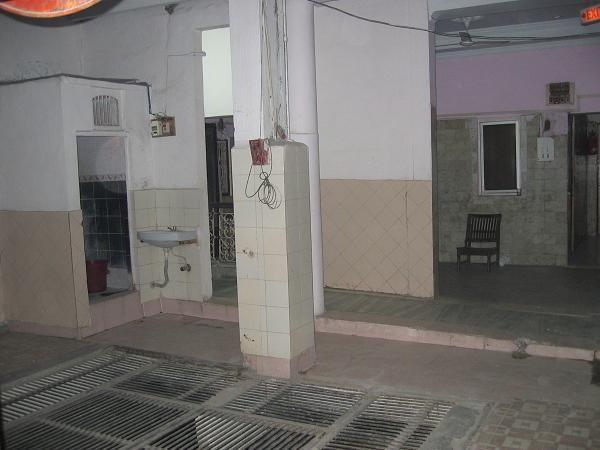
\includegraphics[width=4.8cm]{articles/Arrivee-en-inde/hotel.jpg}

Une petite photo de l'interieur de l'hôtel

\hspace*{-0.65cm}
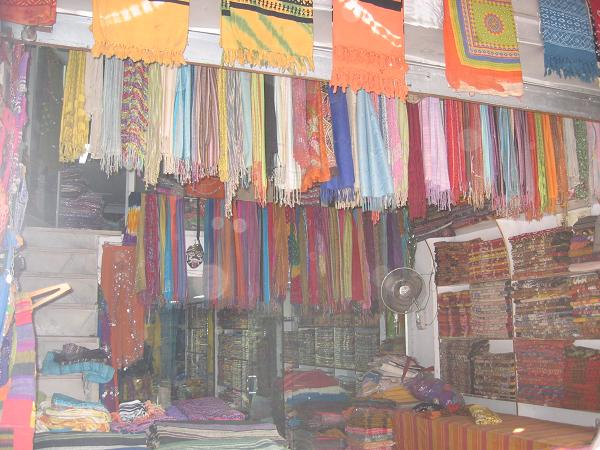
\includegraphics[width=4.8cm]{articles/Arrivee-en-inde/magasin.jpg}

Une boutique de main bazar

\hspace*{-0.65cm}
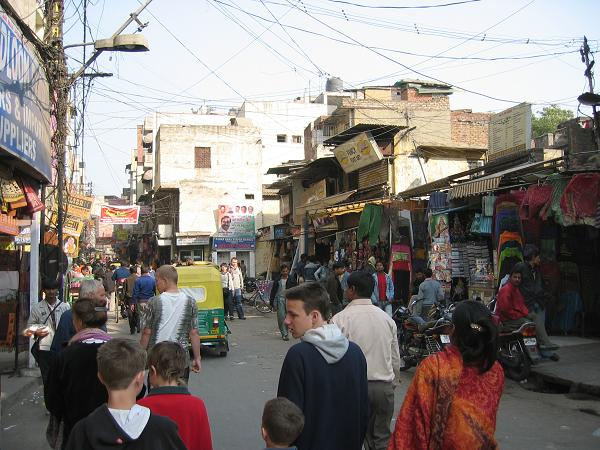
\includegraphics[width=4.8cm]{articles/Arrivee-en-inde/rue.jpg}
L'artère de main bazar, vue de devant l'hôtel

\end{multicols}

\pagebreak\section{Des indiens dans la ville}

1 fév. 2008

\begin{multicols}{2}


Aujourd'hui visite du centre de Delhi et plus spécialement le coin de Connaught Place, tout cela après un petit déjeuner indiano-européen sur le toit de l’hôtel, au 5ème étage, avec vue sur les environs. Une super rencontre au milieu du parc public de Connaught Place avec Raja et Showkat qui nous invitent à prendre un indian tea dans une petite boutique genre snack, nous passons deux heures à discuter avec eux, ils nous ont appris quelques mots d’Hindi qui vont nous être très utiles (on dit namasté pour dire bonjour ou au revoir, ça on le savait, ensuite pour dire merci c’est daniwad et je n’ai besoin de rien se dit chalo). Nous avons alors testé notre nouveau vocabulaire et c’est impressionnant de voire le changement de réaction des gens quand on leur dit un mot dans leur langue. Dire I dont need anything ne sert pas à grand chose alors que dire chalo nous donne droit a un sourire respectueux et aucun insistement de la part du vendeur.

\hspace*{-0.65cm}
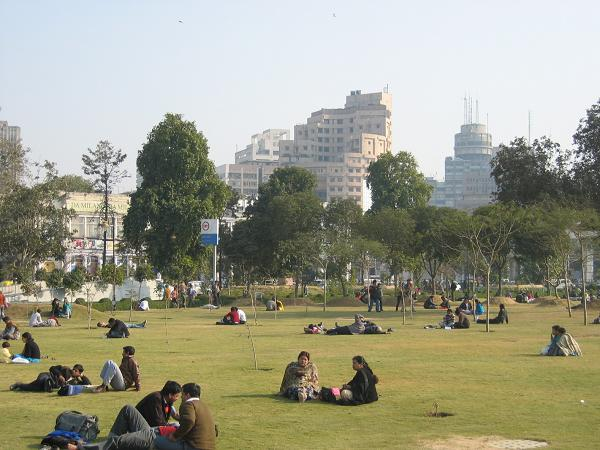
\includegraphics[width=4.8cm]{articles/Des-indiens-dans-la-ville/connaughtplace.jpg}

// TODO : Expliquer la méprise.

Après ça on a essayé de se renseigner sur les trains pour commencer notre tour.
Première boutique, clairement arnaqueuse et habituée aux touristes (d’ailleurs le prix est en euros), mais un chauffeur de rickshaw nous indique une meilleure adresse et il s’agit de la boutique recommandée par le Lonely Planet.

\hspace*{-0.65cm}
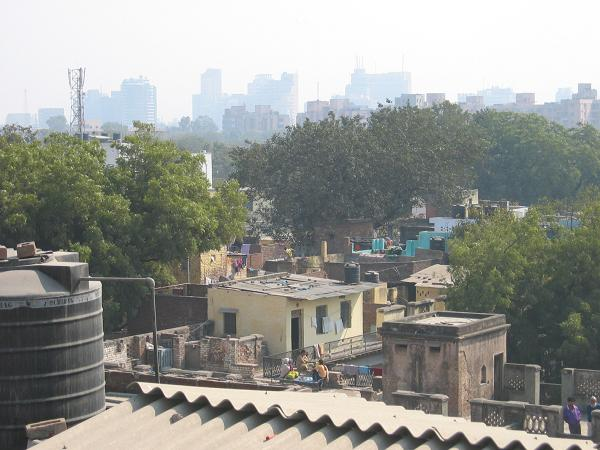
\includegraphics[width=4.8cm]{articles/Des-indiens-dans-la-ville/toithotel.jpg}

Et là... c’est le drame... imaginez le Rajasthan grand comme à peu près deux tiers de la France, mettez y quelques lignes de trains reliant uniquement les grandes villes et une énorme population (12 millions d'habitants à New Delhi). Il faut donc réserver bien a l’avance son trajet, nous n’avons rien avant 12 jours.
On va donc prendre les billets correspondant à la deuxième partie de notre voyage demain et nous devrons nous passer de train pour la première partie (bus, rickshaw...).

\hspace*{-0.65cm}
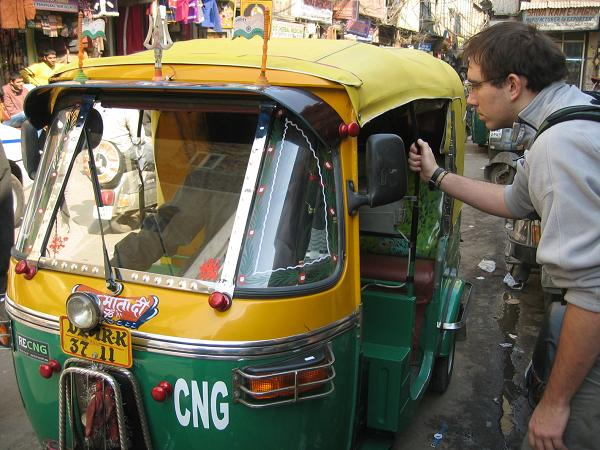
\includegraphics[width=4.8cm]{articles/Des-indiens-dans-la-ville/ricksaw.jpg}

// TODO : Expliquer l'arnaque.

En tout cas niveau repas c’est excellent, et piquant... le respect de l’hygiène est assez folklorique... mais on est pas là pour ça.


\end{multicols}

\pagebreak\bigskip
\textbf{\textsc{Commentaires}}

\medskip
Peggy a écrit le 1 fév. 2008 :
\begin{displayquote}
Ah une photo de d'Etienne, il est vivant!!
Vous êtes très très débrouillards..*impressionée*
Comment dit on "à bientôt" ??
\end{displayquote}

\medskip
Titou a écrit le 1 fév. 2008 :
\begin{displayquote}
Yeah je suis super content de voir que vous vous sentez déjà comme chez vous là bas ! La preuve vous avez déjà fait un troquet ! Bon ok, pour une fois c'était pour boire du thé\dots Mais quand même ! Eclatez vous et à bientôt !
\end{displayquote}

\medskip
Mam' a écrit le 2 fév. 2008 :
\begin{displayquote}
Bien sympa de recevoir un petit coup de fil d'Inde quand on est tout juste réveillée et encore au lit, du coup cela m'a permis de replonger sous la couette pour rêver de Taj-Mahal au lever du soleil, de Jophur(au fait vérifez si la forme des pantalons est bien ce que nous, nous appellons Jodphur!) et de citadelles, palais de maharadjas!!!. Je vous souhaite plein de rencontres. Buvez un lhassi à la santé des blogueurs "Didoum"de notre belle France. Bisou et à bientôt le plaisir de vous lire. Namaste.
\end{displayquote}

\medskip
Tatid a écrit le 21 fév. 2008 :
\begin{displayquote}
Les Indiens ont l'air vraiment accueillants, c'est sympa ça ! J'imagine que vous communiquez en anglais, ça doit être assez drôle un indien qui parle anglais, il doit falloir un temps d'adaptation\dots !
Namaste !
\end{displayquote}

\vfill


\pagebreak\section{Five fingers, not the same}

Date: 03/02/2008

\begin{multicols}{2}

Et oui, Incredible India !

Ce matin, on était parti pour visiter le Taj Mahal, enfin plutôt Mathura en fait, une ville plus au nord, quoique d'un autre côté pas énormement de soleil, donc la balade en rickshaw autour de Agra semblait une bonne idee. Mais alors quand je suis descendue dans la rue ce matin, je suis carrément tombée amoureuse! Agra, chaleureuse, plus calme et colorée que Delhi, très aérée et vivante... c'est décidé, ce sera une balade dans le quartier et puis oh, visite du fameux Taj Mahal (situé dans cette même ville) car le soleil est revenu.

Mais... Incredible India! Petit déjeuner fameux avec vue sur "une larme sur le visage de l éternité" et rencontre avec des jeunes. Ils jouent au cricket, ils sont accueillants et curieux. Merci a Vipin pour la balade sur les toits, la vue imprenable sur le Taj, ses portes et ses fortifications. Cependant attention à ne pas se montrer, les policiers ne permettent pas que les touristes approchent par les toits! Sécurité pour les Indiens nous dit-il. Ils nous protègent, on les écoute, on les respecte. Puis le café indien, en tailleur par terre, avec toujours la vision de rêve, une oeil sur les toits et les rues, le muezzin en fond sonore et le soleil qui caresse la peau.

Quel temps fera t-il le lendemain? Vipin ne le sait pas, son pays est une terre de surprises, Incredible India!

Et les animaux, surprenants eux aussi. Les chiens et les vaches dans la rue, mais aussi les singes sur les terrasses, les écureuils qui pépillent, les rapaces qui paradent. Tout nous émerveille. On discute de beaucoup de choses, on échange sur nos cultures, nos pays. Les photos sont très appreciées, les gens fiers d'être pris et de se voir. Même dans l allée du Taj Mahal, une femme indienne me confie son enfant pour qu'Etienne immortalise le moment. Elle s'approche sans me connaître, me fait confiance, Incredible India!

Et même les femmes en sari, colorées à souhait, posent pour nous, les gens sourient, sont fiers, sûrement heureux d'être là. Nous aussi, on savoure, on se delecte, on profite (et on photographie, pour nous et vous mes amis). Le Taj, imposant monument, les pieds nus sur la pierre puis le marbre, le blanc et le rose, le bâtiment et le fleuve. Mais surtout, surtout, la beauté, le respect, la plénitude. Incredible India!

Demain est un autre jour, et il s'annonce tout aussi beau...

Vous n'avez pas le son, l'ambiance, les gens... Alors profitez bien des images !

To Vipin : We will always keep in mind this point of view : "Five fingers, not the same". Daniwad.

\end{multicols}

\pagebreak\section{Arrivée à Jaipur}

Date: 06/02/2008

\begin{multicols}{2}

Que de choses à raconter...

Premièrement faisons un point sur ce petit début de voyage, nous sommes donc partis de Delhi vers Agra en train, c'est là que nous avons pu voir le Fort rouge et le Taj Mahal, pas gigantesque, mais magnifique, en marbre blanc. Après avoir passé deux jours à Agra nous voulions remonter un peu sur Mathura pour voir les ablussions dans le fleuve Yamuna tôt le matin (les croyants descendent les gaths (escaliers en pierre tombant dans le fleuve) pour se baigner dans le fleuve et ainsi se purifier.

La gare de bus ne nous donnant aucune confiance car il y a trop de personnes ici prêtes à faire monter le touriste dans un mauvais bus pour qu'il soit ensuite obligé de payer un hôtel hors de prix ne sachant pas où il est. Nous avons décidé de prendre le train, en general class (la plus basse des six classes possibles ici, cela se traduit par un entassement de personnes dans un seul wagon, aucune assurance qu'il y ai assez de place, certains sont assis dans les range-bagages au dessus des têtes (je précise que le compartiment bagages n'est pas plus grand que dans un train français en seconde classe, sauf que c'est du grillage).

Malheureusement nous n'étions pas à la bonne saison et seuls les gens de Mathura se baignaient, loins des centaines de personnes que nous nous attendions à voir. Par contre nous avons vu des singes, des singes de partout, surtout tôt le matin. En Inde les singes sont quasiment comme les pigeons à Paris, seulement les Indiens respectent tous les animaux car ils croient en la réincarnation, ne voulant pas tuer un ancêtre potentiel, ils se contentent de les repousser quand ils le peuvent.

Mais Mathura est aussi connue pour être la ville de naissence Krishna, principale incarnation de Vishnu et qui est très vénéré par les Hindous (c'est de là que vient la secte Hare Krishna). Il y avait donc un grand nombre de temples dans cette ville, ainsi qu'une atmosphère religieuse très pesante, nous ne nous sentions pas à notre place c'est pourquoi nous n'y avons passé qu'une nuit.

Le lendemain donc, objectif être à Jaipur le soir, il y avait 300Km à parcourir avec escale à Agra. Retour à Agra en "gen class", puis nous voulions tenter le bus pour Jaipur (l'astuce est que ce bus la ne part pas de la gare routière, nous avions donc plus confiance). Je passe quelques coups de fil à Jaipur pour savoir où dormir, tout est plein, plus le temps, tant pis on part on verra là bas. Seulement les transports ici, on sait quand ca part mais... on sait pas vraiment quand ça arrive, tant mieux on verra bien, si les horaires sont respectés on doit arriver à 22h.

Et la, coup de bol, d'une les horaires sont respectés, et de deux sur la fin du trajet un des passagers nous avait entendu parler francais, il vient nous parler dans cette langue, on lui dit qu'on ne sait pas où on va en sortant du bus, qu'on ne sait pas où s'arrête le bus, "vous voyagez en routard, c'est bien". Il nous indique où aller pour dormir pour pas cher, à deux pas, même pas besoin de prendre un tuk tuk (rickshaw, taxi à trois roues comme sur une des photos d'un post précédent).

Aujourd hui nous avons passé la journée tranquillement dans la ville en se baladant dans les bazaars, qui sont leurs marchés où l'ont peu trouver de tout, des pneus à côté d'une bijouterie, d'un magasin d'étoffes ou d'un vendeur de légumes. Ensuite farniente dans un parc public puis nous voici devant une connection internet des plus lentes qu'il puisse être. nous ne pouvons pas vous mettre de photos aujourd'hui mais promis, pour la prochaine fois.

\end{multicols}

\bigskip
\textbf{\textsc{Commentaires}}

\medskip
Joseph Roubignolles a écrit le 06 fév. 2008 :
\begin{displayquote}
J'aime l'esprit "on tente de planifier tout en sachant qu'on fera autre chose". Je dirais même plus, j'adore ! Que l'esprit du routard veille sur vous et vous guide ...
Bon trip !!
Poutine Spirit
\end{displayquote}

\medskip
Peggy a écrit le 06 fév. 2008 :
\begin{displayquote}
Et je vous ai manqué sur Internet... enfin... l'essentiel c'est que vous avanciez a bon rythme, c'est à dire: le votre.
\end{displayquote}

\medskip
Titou a écrit le 06 fév. 2008 :
\begin{displayquote}
Ro la classe ! J'avoue vous assurez de vous la jouer "guide du routard" qui ne sait pas ou il va ! Franchement respect car je ne sais pas si je pourrais le faire de moi meme ... faudrait que quelqu'un me pousse .. comme un ti dud par exemple :D Ca sera pour le prochain coup ! En tout cas je suis super content de voir que vous en profitez a fond et surtout continuez de vous perdre mais revenez quand meme a la fin ! A bientot les aventuriers et merci de nous faire voyager !
\end{displayquote}

\medskip
Poun's a écrit le 07 fév. 2008 :
\begin{displayquote}
Salut  les 2 explorateurs, merci pour vos nouvelles et votre carte de voyage, mais il est vrai que la seule chose que l'on peut prévoir, c'est que l'on ne peut rien prévoir. Faites Gaaafffe aux arnaaaaques, vous êtes habitués, mais y'a peut-être pire. et plus malins.
Vous pouvez nous ramener une vache sacrée, un singe et 1 l'd'eau du Gange en souvenir?
A bientôt, bon trip....
\end{displayquote}

\medskip
Les vadrouilleurs a écrit le 08 fév. 2008 :
\begin{displayquote}
Merci beaucoup pour vos encouragements, vos commentaires nous font toujours tres plaisir. On voit que certains suivent notre voyage de tres pres.
Continuez comme ca, daniwad.
\end{displayquote}

\medskip
Tatid a écrit le 21 fév. 2008 :
\begin{displayquote}
"les Indiens respectent tous les animaux car ils croient en la reincarnation, ne voulant pas tuer un ancetre potentiel, ils se contentent de les repousser quand ils le peuvent." <= je trouve cette phrase EXCEPTIONNELLE ! Ne voulant pas tuer un ancêtre, trop fort... Forcément avec leur croyance en la réincarnation !
C'est toujours un plaisir de vous lire, bon courage pour la suite !
\end{displayquote}



\pagebreak\section{La vie en Inde...}

Date: 08/02/2008

\begin{multicols}{2}

Nous revoici pour la suite de notre voyage... Nous sommes depuis trois jours à Jaipur, capitale du Rajasthan. Nous avons principalement fait des visites à pieds, nous sommes baladés dans des bazaars en particulier dans la vieille ville, qu'on appelle la ville rose. Puis nous avons rencontré Raj, un jeune qui aide les enfants des rues en leur apprenant la musique, l'anglais, les maths. A la base c'est un artiste, son métier est de faire des spectacles de marionnettes dans des grands hôtels. Nous avons passé une journée complête avec lui et les enfants, il nous a expliqué son projet de construire une école prochainement. C'était impressionnant de voir comment les enfants le considéraient comme leur père. En fait c'est un grand enfant que nous avons rencontré, qui essaie d'aider les autres. Nous essaierons de lui envoyer des fournitures scolaires ainsi que d'autres choses pouvant lui être utiles quand nous rentrerons, avis aux bons coeurs. Entre nos multiples balades dans Jaipur nous avons ensuite visité le palais du vent (Hawa Mahal), façade aux multiples fenêtres destinées autrefois à permettre aux femmes du harem de voir les festivités dans la rue sans être vues. Ensuite nous avons vu le fort de Amber, perché sur une colline dans un cadre magnifique. Les multiples styles architecturaux et la vue depuis le haut nous ont encore fait de beaux souvenirs. En tout cas une chose est sûre, l'Inde nous dépayse complètement et l'on découvre ici plein de choses magnifiques. Jamais vu tant de merveilles au kilomètre carré, qu'il s'agisse des monuments, des rues ou des gens. Chaque journée est riche en émotions. Mais il faut savoir que vivre ici nécessite un temps d'adaptation ainsi qu'une capacité à prendre du recul. En effet, la première chose à savoir est que ici tout se passe dans la rue. Les vendeurs y ont leurs échoppes, les rickshaws, taxis, cyclopouss, motos, voitures, camions, vaches et piétons s'y pressent pêle-mêle, mais surtout les gens y vivent. Enfants à moitié nus, veillards édentés, pères de famille vivent à même le trottoir, sur des couvertures ou sur des charettes. On ne marche donc pas sur le trottoir, par contre on marche sur la route et chacun va où il veut, à ceux de derrière de faire attention. Les bords de route servent aussi de décharge publique. Ici pas de poubelles, on jette tout devant sa porte, et on pousse jusqu'à celle du voisin.

La poussière est omnipresente, le bruit est quasi insupportable de jour comme de nuit. Le klaxon remplace le clignotant et chacun fait ce qu'il veut sans se soucier de l'autre, comme hurler dans la rue à 3h du mat ou jouer du drum à cote de quelqu'un qui dort (et quand on a une chambre dont les fenêtres ne ferment pas, on peut vous dire que c'est pas très tranquille les nuits). Le temps est une notion toute relative ici, de même que la propreté. La cuisine des petits restaurants est dehors, sur le trottoir, sans murs ni aucune protection, les cafards se baladent sur les murs sans complexes, les chambres d'hôtel sont poussiéreuses, les salles de bain heu... bof. Mais pour nous pas de soucis, on n'y prête plus vraiment attention. Et les animaux, partout il y en a, pour nous c'est incroyable. Outre les vaches sacrées qui se baladent sur les routes et que les voitures évitent soigneusement, de nombreux chiens et chèvres vivent dans la rue. On trouve aussi beaucoup de poules, de singes, d'écureuils, d'oiseaux. Les rats eux préfèrent quand même les gares aux rues, c'est déjà ça.

La nourriture, c'est aussi quelque chose. Très bon, mais très épicé. On a par contre un peu de mal à s'y faire et on commence à reprendre des habitudes alimentaires occidentales : le riz presque nature pour tenir au ventre, le coca pour aider à la digestion et boire autre chose que de l'eau purifiée aux pastilles, les oeufs au plat et beurre confiture au ptit dej, les chips Lays pour le coup de faim et ce midi, le Mac Do. Tant d'autres choses à raconter, mais le principal est déjà dit et permet de brosser l'atmosphàre générale, car la vie ici se vie évidemment bien au delà de nos visites touristiques. Ah oui, encore une chose trèèès importante ici : les arnaques ! 100\% du temps les gens cherchent à nous arnaquer, alors il faut savoir déjouer les pièges, et surtout ne jamais faire totalement confiance et toujours anticiper. Evidemment, il y a les prix qu'il faut marchander, mais aussi les rickshaws qui nous arrêtent où ils veulent pour avoir du backchich à la boutique ou nous faire acheter des légumes pour faire de la monnaie. Les offices de tourismes ou bureaux de tourisme en tout genre envoient vers des hôtels hors de prix ou vendent des tickets de train trois fois leur valeur. Les boss des hôtels nous montrent la chambre la plus pourrie d'une gamme pour que l'on prenne la gamme au dessus, les gentilles personnent qui aiment bien les francais et demandent à ce qu'on traduise une lettre de remerciement en Français sont invariablement commercants... impossible d'écrire toutes les arnaques auxquelles on a droit, mais tout ça pour dire que c'est pas de tout repos. Cela dit, les enfants qui viennent nous voir sont juste fiers et heureux de pouvoir nous dire "hello, what is your name, how are you" en nous serrant la main et nous font des sourires magnifiques. On nous aborde souvent juste par curiosité "From which country ? Oh France, so you are from Parissssse ?"

\hspace*{-0.65cm}
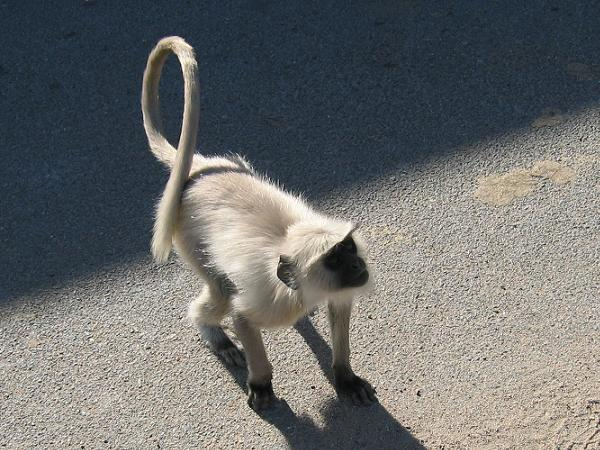
\includegraphics[width=4.8cm]{articles/La-vie-en-inde/singe.jpg}
Un macaque.

Allez les gens, à la prochaine.

\end{multicols}

\bigskip
\textbf{\textsc{Commentaires}}

\medskip
Peggy a écrit le 8 fév. 2008 :
\begin{displayquote}
C'est magique ton récit.
\end{displayquote}

\medskip
Titou a écrit le 8 fév. 2008 :
\begin{displayquote}
Toujours un grand plaisir de vous lire (au boulot) ! C'est vrai que ça a l'air d'être un univers complètement différent. J'ai beau être parti loin il n'y a rien de comparable. Faites gaffe à vous quand même avec les ti soucis sanitaires et surtout profitez toujours à fond de cette super expérience que vous êtes en train de vivre ! Merci de nous la faire partager. A très bientôt ! Biz à vous deux !
\end{displayquote}

\medskip
Poun's a écrit le 8 fév. 2008 :
\begin{displayquote}
C'est super de pouvoir partager un peu de votre expédition grâce aux commentaires et aux photos. Je pense qu'on est pas mal à attendre impatiemment le prochain épisode!
A bientôt.
\end{displayquote}

\medskip
Sam a écrit le 9 fév. 2008 :
\begin{displayquote}
Pfiou :) Je vous admire de mener une telle aventure ! Je ne pense pas pouvoir survivre à ça pendant plus de 48h.
En tout cas, vous voyez et vivez des choses magnifiques, c'est le principal ! Continuez à déjouer les arnaques et à vous en prendre plein la vue pour nous tous !
\end{displayquote}

\medskip
Les vadrouilleurs a écrit le 10 fév. 2008 :
\begin{displayquote}
Merci beaucoup pour vos messages, c'est vrai qu'on nous avait prévenu qu'on se prendrait une grosse claque en arrivant ici, et heureusement d'ailleurs car sinon\dots
\end{displayquote}

\medskip
Seb a écrit le 11 fév. 2008 :
\begin{displayquote}
Super sympa de nous faire partager tous ça, ça a l'air d'être super impréssionant là bas.
Bonne suite et que l'aventure continue.
\end{displayquote}

\medskip
Catherine a écrit le 11 fév. 2008 :
\begin{displayquote}
Vous me donnez de plus en plus envie de partir en Inde en juillet. Mais j'attends votre avis : est-ce profitable pour François et Marine ou faut-il attendre qu'ils soient plus agés ?
métier oblige : je suis sensible à la demande pour les écoliers et aimerais savoir ce qu'il est souhaitable d'envoyer et à quelle adresse ? (en recommandé où le facteur ne risque pas de se servir ?)
Vous nous transmettrez l'adresse à laquelle on vous enverra un peu d'argent quand les arnaques auront eu raison de votre porte-monnaie\dots
merci beaucoup à Cécile pour son appel.
\end{displayquote}

\medskip
La vadrouilleuse a écrit le 13 fév. 2008 :
\begin{displayquote}
Pour répondre au dernier commentaire, voici notre avis sur le fait d'emmener des enfants en vacances en Inde. On est catégoriques, d'apres notre expérience, non, les enfants restent à la maison. Trop de choses ici peuvent heurter leur sensibilité et les marquer à vie.
De même qu'une femme seule, ou meme deux jeunes femmes, ou une femme et ses enfants seront ici, on pense, sans arrêt regardés et il vaut mieux s'abstenir de voyager dans ces conditions. La condition de la femme n'est pas la même ici qu'en Europe.
\end{displayquote}

\medskip
Tatid a écrit le 21 fév. 2008 :
\begin{displayquote}
Je le disais dans un commentaire précédent (ou suivant plutôt puisque je lis le blog dans le sens non-chronologique :p), niveau confort et culture, ça doit faire un méga choc, surtout pour nous occidentaux qui avons besoin d'une certaine hygiène quoi\dots C'est vrai que je serais méfiant quant à la nourriture que je pourrais manger\dots
Sinon, vue comment vous décrivez ce qui se passe dans la rue, ça doit être un sacré bordel :-D Quant aux arnaques, je trouve ça abusé, profiter des touristes pour leur faire cracher de la thune tout le temps, grrr\dots
Félicitation quand même d'avoir eu le courage de vivre cette aventure (qui en est vraiment une en soi) !
Grâce à ce voyage, d'après ce que vous racontez, vous avez rencontré des gens assez exceptionnels, je pensais à Raj là, c'est génial ce qu'il fait pour les autres, ça doit être touchant de voir ces enfants pris en charge par un "grand enfant" qui veut leur apporter de la connaissance\dots J'ai hâte de voir les photos !
\end{displayquote}

\vfill


\pagebreak\section{Journées zen}

11 fév. 2008

\begin{multicols}{2}

Après Jaipur, 2h30 de bus et nous voila à Ajmer, petite ville de 250.000 habitants si nos souvenirs sont bons. Le principal avantage du lieu est de se situer sur de nombreuses lignes de bus et d'être à seulement 15 km de Pushkar, ville de pèlerinage, très réputée pour sa beauté. Nous n'y avons donc passé qu'une nuit et qu'une journée. Toutefois nous en avons profité au maximum pour nous balader, prendre le soleil et admirer le paysage. Tout d'abord, visite du Temple Rouge Jaïn, qui nous a révélé une magnifique maquette de ville aux bateaux flottants dans les cieux, le tout recouvert de 500kg de feuillles d'or. Les murs étaient même sculptés en colonnes brillantes de vert, de rouge, de bleu.

Nous avons continué notre route jusqu'à un fort non loin. Il s'agit d'un musée contenant des tablettes de pierres gravées d'écritures et de scupltures à l'effigie des dieux. La cour intérieure était tellement verdoyante et paisible que nous y avons déposé nos sacs pour une halte détente, farniente et bouquinage. L'Inde, lorsqu'elle est calme, est propice au repos et à la reflexion. Le lac fut notre dernière visite dans cette ville. Le parc est accueillant et vivant, les quais sont en marbre avec des autels et l'eau calme reflète les montagnes environnantes. Premier changement radical de décor pour nous, ça ressemble plus au désert.

Le soir pour venir à Pushkar nous avons comme à notre habitude pris le bus. Enchantés dès l'arrivée par la petite bourgade de 15.000 habitants (ou plutôt ce qu'on arrive à en voir entre la station de bus et le premier hôtel où l'on entre), nous avons pu profiter de la suite du spectacle lors d'une balade dans le bazar, encore baigné de soleil. De retour le soir, on constate avec ravissement que notre hôtel porte bien son nom de Lake View. La terrasse (qui est le toît, je pense que vous l'aurez compris, comme partout en Inde) offre une vue imprenable sur le lac sacré de Pushkar, où viennent se baigner de nombreux fidèles. A cette heure, le soleil se couche, libérant des lueurs jaunes, oranges et violettes dans le ciel, l'eau est tranquille, les montagnes presque bleues et les lumières de la ville commencent à s'allumer. Nous restons là un long moment à admirer le soleil qui descend puis s'éteint. Le soir, repas autour du feu en compagnie d'un Français et des Indiens du restaurant sur fond de Bob Marley. Ce fut une journée tout à notre rythme, très agréable.

Aujourd'hui aussi, du coup, nous en avons profité juste en marchant, en faisant quelques emplettes et en profitant de la terrasse de l'hôtel. J'ai eu la chance, mais aussi l'audace de rentrer dans un temple, d'offrir des fleurs à Krishna et de lui faire une offrande de fleurs dans l'eau du lac. C'est une expérience qui je crois m'a beaucoup marquée, surtout moi qui suis si émotive, j'ai été très touchée.  Maintenant que la nuit est tombée, nous avons profité de cette ambiance si différente pour faire un saut jusqu'ici vous donner des nouvelles et vous montrer quelques photos.

\smallbreak
\hspace*{-0.65cm}
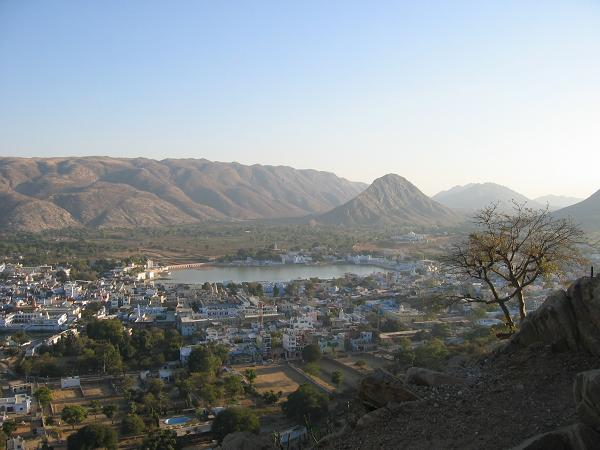
\includegraphics[width=5cm]{articles/Journees-zen/pushkar.jpg}
%La ville de Pushkar.
\smallbreak

\end{multicols}

\bigskip
\textbf{\textsc{Commentaires}}

\medskip
Titou a écrit le 11 fév. 2008 :
\begin{displayquote}
Salut la jeunesse ! J'attendais avec impatience la suite de vos peripeties et comme d'habitude c'est avec une grande joie que je vous lis ! A vous lire ca fait rever et donne vraiment envie de repartir encore plus loin pour un choc de culture encore plus gros ! Je pense que vous plannez complet labas avec ce que vous voyez et je vous souhaite de continuer ca jusqu'au bout ! Merci pour ces news et a tres vite ! Biz a vous deux.
\end{displayquote}

\medskip
Lydie a écrit le 12 fév. 2008 :
\begin{displayquote}
De mon petit bureau monotone, je m'évade grâce à vous !
Je suis subjuguée par les aventures que vous vivez !!!
Vous vivez une aventure qui restera à tout jamais gravé dans vos mémoires.
Ma petite Cécile, je dois t'avouer que je t'admire. Je suis bien incapable de partir ainsi à l'aventure (mon petit confort m'est si indispensable !).
Mais je dois également avouer que je t'envie, j'aimerais tenter et pouvoir être fier de l'avoir vécu !!!
Voir une culture si différente avec des besoins qui sont réels, doit donner une grande leçon d'humilité !
Vous reviendrez j'en suis sûre, avec une autre vision du monde et ça ne peut être que constructif !
Tu vas ainsi pouvoir relativiser des mésaventures que l'on peut connaitre dans notre palais occidental doré qu'est la France !
Mon esprit sécuritaire me pousse tout de même à vous dire de faire attention et de bien prendre soin de vous (sanitaire et sécuritaire)!
BRAVO à toi ma petite Cécile, ma petite routarde !
Je vous souhaite bonne route, profitez de chaque instant et remplissez votre mémoire de chaque moment, ce sont les seuls souvenirs qui resteront à jamais aussi fort !
Merci de nous faire partager ces moments
J'attends avec impatience vos prochains récits
Grosses bises à vous 2 et prenez soin de vous !
Lydie
PS : Je suis bien évidemment partante pour vous donner de l'aide afin que ces enfants aient accès à l'enseignement et autres\dots
\end{displayquote}

\medskip
Poun's a écrit le 12 fév. 2008 :
\begin{displayquote}
Salut les z'aventuriers. Ca fait plaisir d'avoir de bonnes nouvelles. Des images de plus en plus belles, continuez comme ça, profitez bien, mettez-en plein votre tête!
Coucou à Lydie en passant et message à toutes et tous :
On ne pose pas de questions techniques, on les laisse vivre leur trip et on leur tombera dessus lorsqu'ils seront rentrés! Ils en auront pour un bon moment à nous raconter.
A bientôt pour la suite\dots
\end{displayquote}

\medskip
Tatid a écrit le 21 fév. 2008 :
\begin{displayquote}
Snif, j'arrive trop tard pour voir les photos, c'est de ma faute, j'avais qu'à lire le blog avant :-p
Rien que vos descritions nous laissent imaginer des paysages et monuments superbes !
\end{displayquote}

\vfill


\pagebreak\section{Descente vers Udaipur}

13 fév. 2008

\begin{multicols}{2}

Heu... on vient de passer plusieurs jours à se dorer la pilule sur le toit de l'hôtel et se balader. Que dire de plus sinon que tout va pour le mieux! On devrait entamer ce soir notre descente en bus vers Udaipur, soit 10 heures de trajet. On éspère avoir des couchettes, sinon on fera comme d'hab, c'est à dire on changera nos plans au dernier moment (oui oui vous avez bien lu, un bus avec couchettes).

On éspère que pour vous tous tout se passe bien. Namasté.

\end{multicols}

\bigskip
\textbf{\textsc{Commentaires}}

\medskip
Titou a écrit le 13 fév. 2008 :
\begin{displayquote}
Ba alors la pour etre court il est court votre post ! Bon voyage en bus 4 etoiles (ba oui y a les couchettes :D) et tenez nous au courant quand vous serez arrives ! Bisous a vous deux et a ploutch les namis.
\end{displayquote}

\medskip
Lydie a écrit le 14 fév. 2008 :
\begin{displayquote}
Ah ben moi qui m'impatientait de lire vos péripéties, je reste sur ma fin ...
Je rigole
J'espère que vous avez bien eu votre bus à couchette !!!
Merci ma poulette pour ta carte, ça nous a fait drolement plaisir et ça nous donne bien évidemment envie de partir (peut être pas autant à l'aventure que vous !!!)
faites attention
Bisous à vous
\end{displayquote}

\medskip
Poun's a écrit le 15 fév. 2008 :
\begin{displayquote}
Salut vous deux! Merci pour la carte. Etienne, tu ne t'es pas fatigué, tu aurais au moins pu la signer! On réglera ça quand vous serez rentrés...
J'espère que tout va bien et que vous profitez un max.
A bientôt pour de nouvelles aventures.
Question aux lectrices et lecteurs de ce blog : je ne peux plus charger les images de la page "Five fingers, not the same". Et vous, avez-vous toujours ces images?
A bientôt tout le monde, Bernard
\end{displayquote}

\medskip
Titou a écrit le 15 fév. 2008 :
\begin{displayquote}
Non les images ne marchent plus .... ça fait très sérieux pour le blog de deux ingénieurs INFORMATICIENS :D enfin moi je dis ça je ne dis rien .... Biz les amis
\end{displayquote}

\medskip
Nous deux a écrit le 16 fév. 2008 :
\begin{displayquote}
Alors qu on vous explique...
Le blog a ete termine de coder une ou deux heures avant de partir... exams obligent. Du coup tous les tests n ont pas pu etre faits et on a eu un probleme pour mettre les photos des les premiers posts, donc il a fallu trouver un autre endroit ou les mettre sur le net et vous faire des liens sur le blog. Ce qu on savait pas c est que les photos sont stockees 15 jours uniquement, donc elles disparaissent petit a petit. Pas de souci on essaie d arranger ca depuis l'inde.
\end{displayquote}

\medskip
Tatid a écrit le 21 fév. 2008 :
\begin{displayquote}
Certaines se dorent la pillule sur les toits des hôtels en Inde pendant que d'autres se caillent les c*uilles en costar dans les rue Parisiennes venteuse (je sais pas si ce mot existe, donc voilà la signification : avec du vent !), la vie est injuste :-p !
Pfff, ça y est, j'ai envie de voyager, votre blog et celui de Fab m'ont trop donné envie... ! Profitez bien !
\end{displayquote}

\vfill


\pagebreak\section{Octopussy}

Date: 16/02/2008

\begin{multicols}{2}

Alors... nous étions restés à Pushkar, Nous avons pris le bus pour Ajmer dans l'après midi il y a trois jours pour ensuite voir les horaires de bus pour Udaipur, de nuit. Le notre est à 23h30, on tue le temps en attendant. Ca y est, le bus est là... mais il n'a pas de couchettes comme on nous avait fait comprendre. Durée annoncée : 8h, sauf qu'en fait c'était 5h30. Arrivée donc à 5h du matin à Udaipur, il gèle, il faut qu'on trouve un endroit pour finir la nuit.

Par la suite, visite d'Udaipur et de jour, c'est beaucoup plus agréable qu'a 5h, si si... Udaipur est assez vaste, cependant la majorité des choses à voir se trouve dans un petit quartier, au bord du lac Pichola. Dans ce quartier nous avons vu un temple Jain.

\hspace*{-0.65cm}
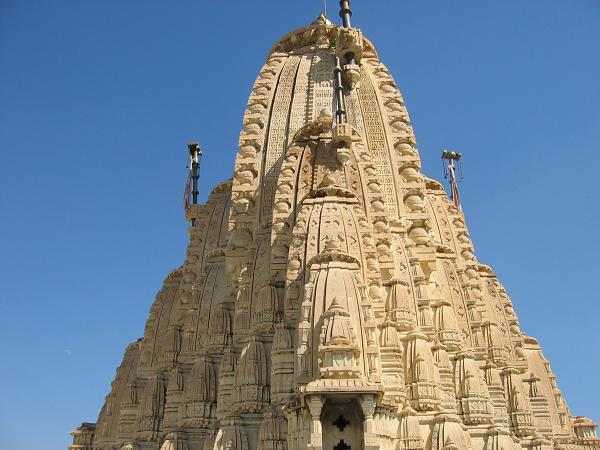
\includegraphics[width=4.8cm]{articles/Octopussy/jain.jpg}
Un temple Jain

Puis nous avons visite le City Palace, d'où la vue sur la ville est superbe.

\hspace*{-0.65cm}
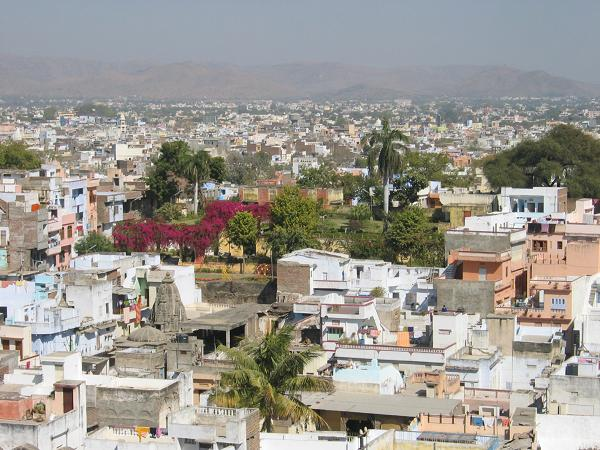
\includegraphics[width=4.8cm]{articles/Octopussy/zoomville.jpg}
Vue sur la ville

Udaipur est aussi connu pour avoir servi de décor au tournage du film Octopussy, James Bond. C'est un luxueux hôtel en plein milieu du lac qui est filmé.

\hspace*{-0.65cm}
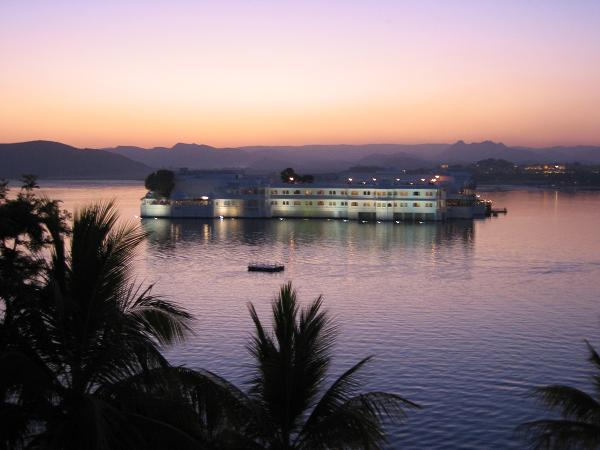
\includegraphics[width=4.8cm]{articles/Octopussy/octopussy.jpg}
Hotel de James Bond

Et pour finir cet article, voici un magnifique coucher de soleil sur le lac.

\hspace*{-0.65cm}
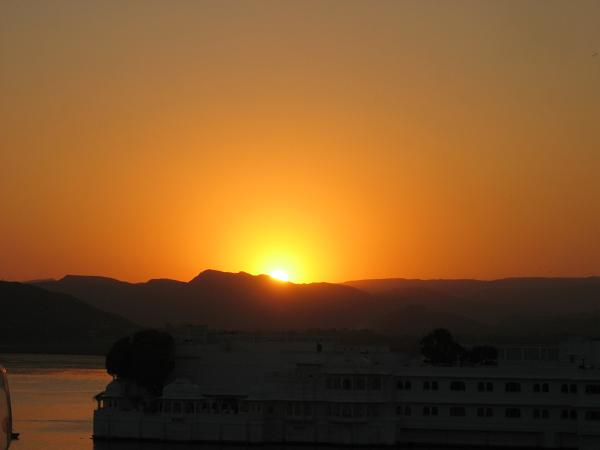
\includegraphics[width=4.8cm]{articles/Octopussy/soleil.jpg}
Coucher de soleil

A bientôt...

\end{multicols}

\bigskip
\textbf{\textsc{Commentaires}}

\medskip
Poun's a écrit le 16 fév. 2008 :
\begin{displayquote}
Ouah, toujours de belles images. Pas trop dur, les voyages dans les bus-couchettes sans couchettes?
Une arnaque de plus? Faites toujours attention, et faites toujours le plein d'émotions.
Les photos où tu avais l'enfant dans tes bras et toutes celles de cette page (five fingers, not the same) ont disparu. Incident technique ou censure?
Par prudence, évitez de transmettre des photos trop personnelles de vos guides et de vos contacts, et ne racontez pas sur le net les épopées pas très licites.
Mais à part ça, profitez!
A bientôt pour un nouvel épisode!
\end{displayquote}

\medskip
Jean yves a écrit le 16 fév. 2008 :
\begin{displayquote}
Je suis pas à pas votre périple,sur sur carte de l'atlas au 1/450000.Vu là dessus c'est impresionnant qu'il faille toute une nuit pour aller de Almer à Udaipur.Au Laos,nous avions ainsi pris un bus toute une nuit à travers la montagne.Ceux qui dormaient n'avaient pas vu les précipices,les villages traversés à une vitesse folle.

Question culturelle: qu'est ce qu'un temple Jain?
Nouvelles de la famille : ce soir à 10h,toujours pas de petite fille en vue à Besançon .
Bravo les photos, et le texte. c'est agréable à lire.
Juste: J'imagine que vous n'osez pas trop prendre les gens en photo. Nous non plus..c'est pourtant bien sûr ce dont on se souvient le plus après...J'ai envie de voir les Indiens.
\end{displayquote}

\medskip
Titou a écrit le 17 fév. 2008 :
\begin{displayquote}
Encore un joli article avec de magnifiques photos ! J'avoue le coup du bus sans couchettes c'était pas top comme surprise mais bon je pense que vous avez survécu sans trop de problèmes ! Profitez en toujours a fond et surtout faites gaffe à vous !
\end{displayquote}

\medskip
Annie et Jean-yves a écrit le 17 fév. 2008 :
\begin{displayquote}
EH,bien nous on va faire aussi un super voyage :
vers Besançon et vers une petite fille qui est en train de faire son arrivée sur la terre dans les heures qui viennent...On est trop contents.Bisou à tous les blogueurs Didoum,ceux qu'on connait et les autres.
\end{displayquote}

\medskip
Etienne a écrit le 17 fév. 2008 :
\begin{displayquote}
Alors, pour ceux qui n'auraient pas compris je viens d'etre tonton ce matin, j'en connais deux qui doivent etre sur un petit nuage, du cote de Besancon. Felicitation p'tite soeur et a toi aussi Jef...
Passons a la page culture : Le Jainisme
Voici le debut de la definition du Jainisme prise sur wikipedia : Le jaïnisme, ou jinisme, du sanskrit Jina «vainqueur», est une religion (en précisant que le mot religion se traduit en Inde par dharma, un mot largement polysémique qui signifie autant «foi», «religion», «vertu» que «devoir», «nature propre», «bonne action»...), un chemin spirituel qui insiste sur les concepts d'ahimsa (non-violence) et de karma et qui met l'accent sur l'ascétisme.
Pour la definition complete, <a href="http://fr.wikipedia.org/wiki/Jainisme">cliquez ici</a>.
\end{displayquote}

\medskip
Titou a écrit le 18 fév. 2008 :
\begin{displayquote}
Hey hey félicitation mon pti DUD tu es tonton ! Félicitation aussi aux parents (car c'est quand même eux qui ont fait tout le boulot :D )  et aux grands parents ! Une excellente nouvelle ça ! Ça va pouponner fort du coté de Besançon ! Bisous à tous !
\end{displayquote}

\medskip
Lydie a écrit le 18 fév. 2008 :
\begin{displayquote}
Félicitation à Etienne !
Je me répéte par rapport aux autres, mais pas mal le bus couchettes sans couchettes !!!
Les photos sont magnifiques! Vos péripéties donnent vraiment envie de faire le sac et de partir!
Profitez bien
Je pense fort à toi ma poulette !
Gros Bisous
\end{displayquote}

\medskip
Tatid a écrit le 21 fév. 2008 :
\begin{displayquote}
Félicitation nouveau tonton :-)
Ah ouais les transports, ça doit être un peu long quand même, 5h30 en bus pendant la nuit, ça doit pas être super confort quoi, mais bon, c'est le charme du pays ;-)
Je pensais à un truc, vous mettez le blog relativement à jour avec des photos et tout et tout, chapeau, pcq là-bas, je sais pas si vous trouvez facilement des cyber-café ?!
Allez, zou, j'ai d'autres photos à voir et d'autres articles à lire !
Bisous à vous deux !
\end{displayquote}

\vfill


\pagebreak\section{Il commence à faire chaud}

18 fév. 2008

\begin{multicols}{2}

Aujourd'hui, je vais vous livrer un petit secret : nos 3 phrases préférées du moment :
- "Dure la vie hein!", à prendre évidemment au second degré. On dort dans des hôtels sympa, on mange dans des restos très bons avec des vues exceptionnelles, le petit vent chaud du soir est très agréable, les palaces sont plus beaux les uns que les autres...
- "Ca fait combien de temps qu'on n'a pas vu un nuage?" La réponse commence à s'approcher gentiment de "deux semaines". Et oui, que du grand ciel bleu à l'horizon, du lever au coucher du soleil (qui sont toujours rouges, bleus, verts et violets on tient à préciser).
-"Ils sont fous, vraiment, complètement fous je te dis". Les Indiens bien sûre, on n'a pas idée de construire autant de merveilles au kilomètre carré. Les yeux grands ouverts on arrive toujours pas à tout capter ce qui se présente devant nous. Toutes les sculptures, tous les détails, le zèle des batisseurs... c'est incroyable.

Et au dela de ces impressions générales qui se confirment de jour en jour, nous continuons notre périple. Nous avons quitté notre hôtel ce matin à 5h, puis 3 grosses heures de bus pour arriver à Ranakpur. Là se trouve un des plus importants temples Jain de l'Inde, plus trois autres plus petits. Le gros comprends 29 pièces, et pas moins de 1444 colonnes de marbres sculptées (oui ils sont fous, on vous avait bien dit hein!). Les temples sont encastrés entre les montagnes, toutes recouvertes de verdure. On a même le plaisir de nourir les singes qui viennent calmement prendre des morceaux de gâteaux qu'on leur tend. Encore une halte fort agréable. Le soir, 4h30 de bus pour rejoindre Jodhpur où nous sommes actuellement. Ca semble promettre des moments sympa, surtout que nous allons y rester 5 ou 6 jours, jusqu'au moment de rentrer à Delhi pour faire des achats et prendre l'avion de retour. Et oui, on va être obligés de rentrer au bout d'un moment! En tout cas, on ne pense pas encore vraiment à ça et on profite à fond de chaque petit moment, de tout ce qui peut nous émerveiller : un oiseau vert et orange, des femmes rentrant des champs portant des fagots sur leur tête, des maisons de toutes les couleurs, les femmes qui lavent le linge sur les ghats... Nous passons tellement de moments intenses et indescriptibles! Le City Palace d'Udaipur qui s'illumine le soir, un spectacle de danse rajasthanie , la rencontre d'Indiens, mais aussi d'autres touristes, Européens, Américains ou encore Francais. On comprend de mieux en mieux l'anglais des Indiens et on relance les conversations. Nous croisons beaucoup de gens, mais brièvement. Nous nous fondons aussi de mieux en mieux dans le paysage, portant des habits plus "cool" et connaissant maintenant les combines des marchands. On ne prévoit plus ce qu'on fait, mais seulement on vit le moment à fond. Car l'Inde est un pays qui ne se raconte pas, mais qui se vit. Les photos sont peut-être jolies et les textes vous plaisent, mais tout ça n'est rien du tout par rapport à la réalité que nous vivons avec un grand plaisir chaque jour, chaque minute. Souvent les mots manquent pour exprimer ce que l'on ressent. On se contente alors d'un silence, d'un regard entre nous et d'un large sourire tout au fond du coeur. On ne réinventera pas les mots, nul besoin, car on sait très bien au fond de nous l'effet que ça produit, la trace que ça laissera, et c'est bien le principal.

%\hspace*{-0.65cm}
%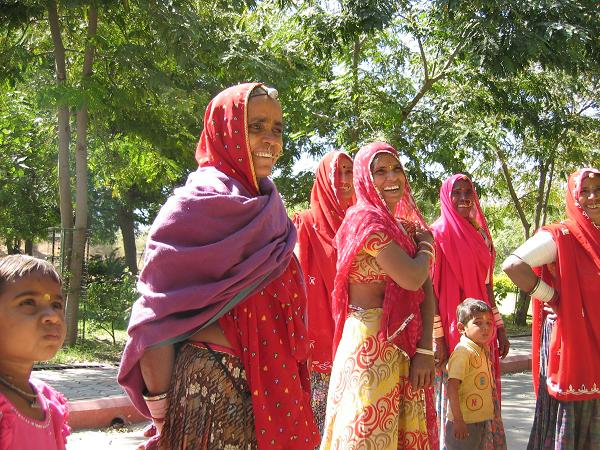
\includegraphics[width=4.8cm]{articles/Il-commence-a-faire-chaud/sari.jpg}
%Des femmes en sari coloré

%\hspace*{-0.65cm}
%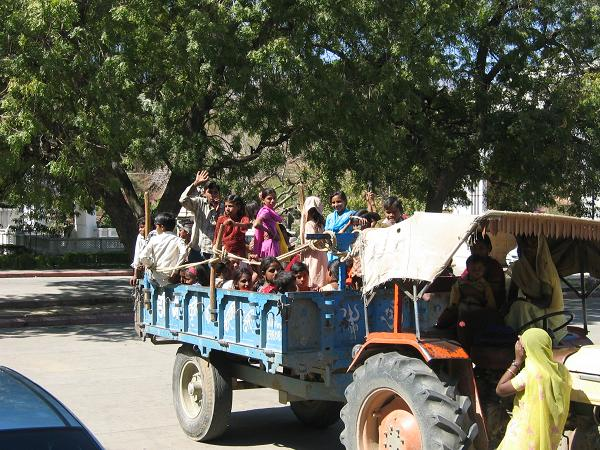
\includegraphics[width=4.8cm]{articles/Il-commence-a-faire-chaud/scolaire.jpg}
%Un groupe d'enfants en sortie scolaire.

%\hspace*{-0.65cm}
%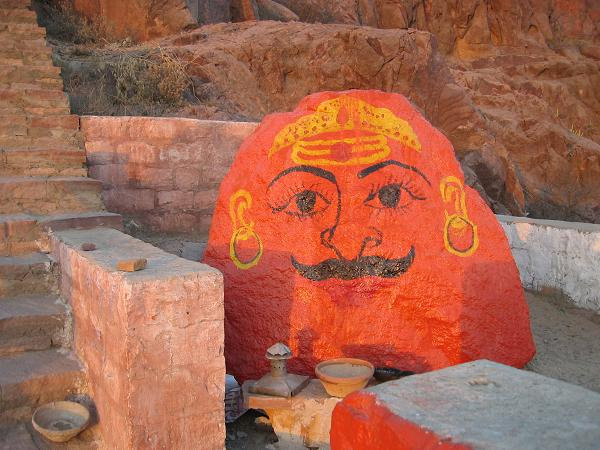
\includegraphics[width=4.8cm]{articles/Il-commence-a-faire-chaud/bonhommerouge.jpg}
%Une icône peinte sur un rocher.

%\hspace*{-0.65cm}
%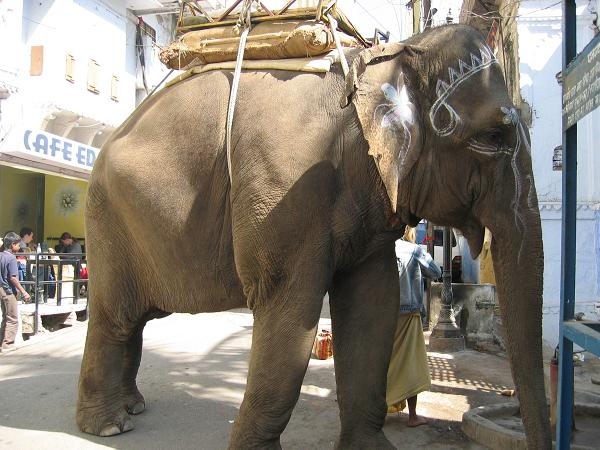
\includegraphics[width=4.8cm]{articles/Il-commence-a-faire-chaud/elephant.jpg}
%Un éléphant dans une rue d'Udaipur.

%\hspace*{-0.65cm}
%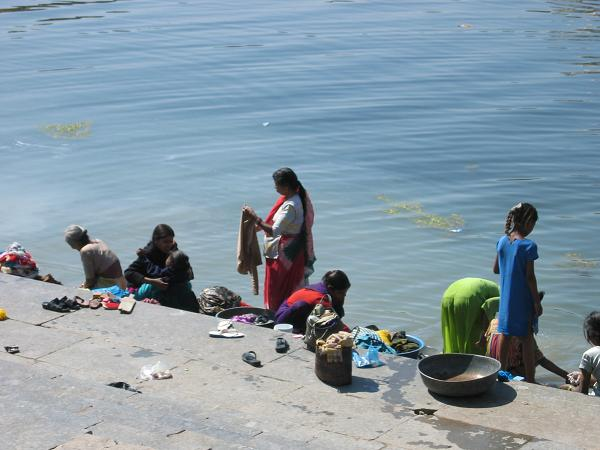
\includegraphics[width=4.8cm]{articles/Il-commence-a-faire-chaud/linge.jpg}
%Des femmes lavant le linge sur les gaths.

%\hspace*{-0.65cm}
%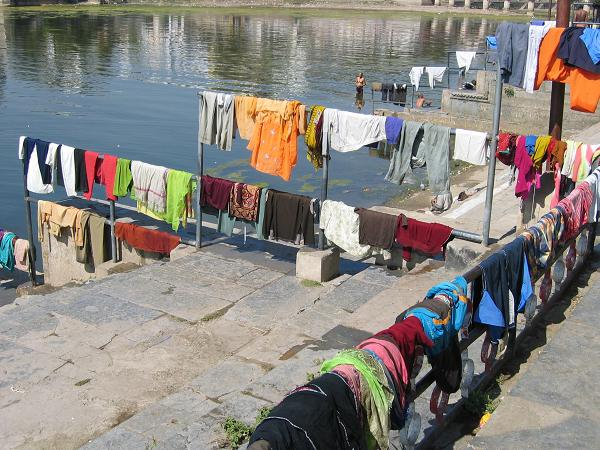
\includegraphics[width=4.8cm]{articles/Il-commence-a-faire-chaud/seche.jpg}
%Le linge qui sèche.

%\hspace*{-0.65cm}
%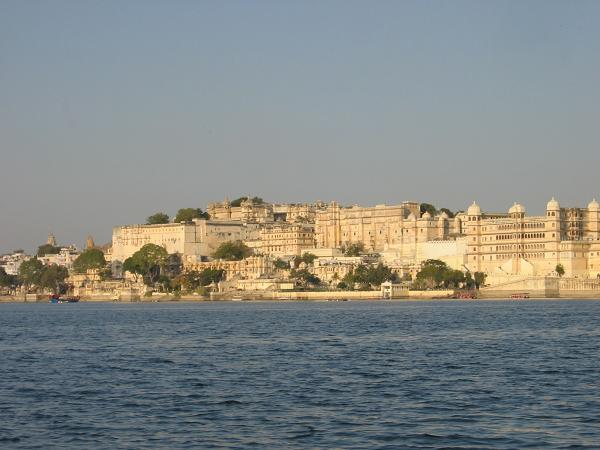
\includegraphics[width=4.8cm]{articles/Il-commence-a-faire-chaud/palacelac.jpg}
%Le City Palace d'Udaipur vu depuis le lac.

%\hspace*{-0.65cm}
%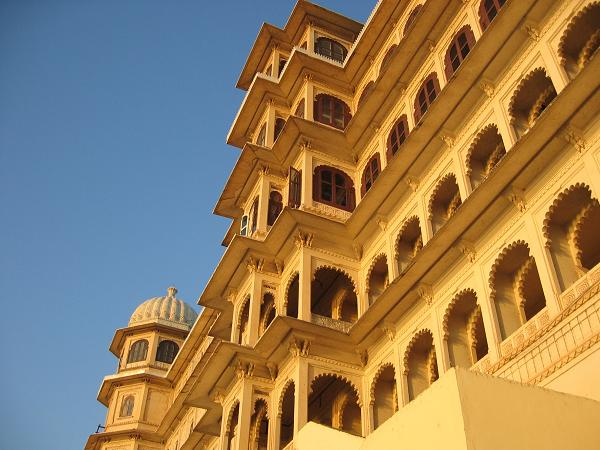
\includegraphics[width=4.8cm]{articles/Il-commence-a-faire-chaud/citylac2.jpg}
%Une autre vue du City Palace.

%\hspace*{-0.65cm}
%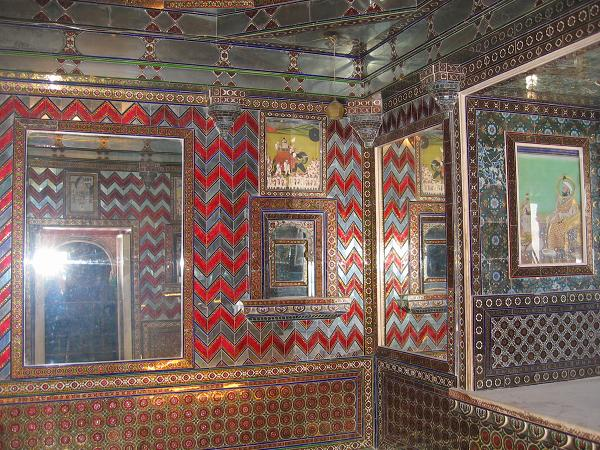
\includegraphics[width=4.8cm]{articles/Il-commence-a-faire-chaud/citysalle.jpg}
%Une salle du City Palace.

%\hspace*{-0.65cm}
%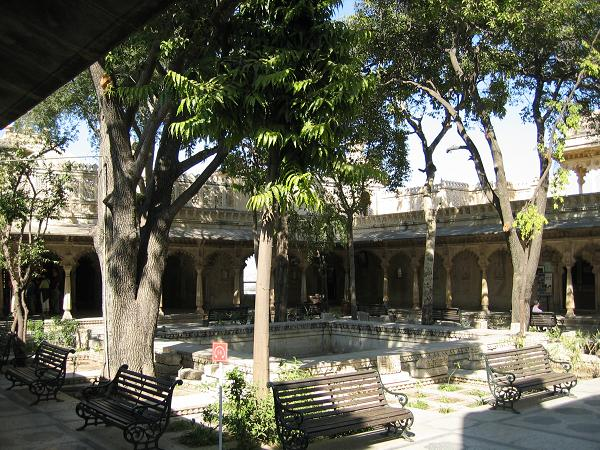
\includegraphics[width=4.8cm]{articles/Il-commence-a-faire-chaud/citycours.jpg}
%Une cour intérieure.

%\hspace*{-0.65cm}
%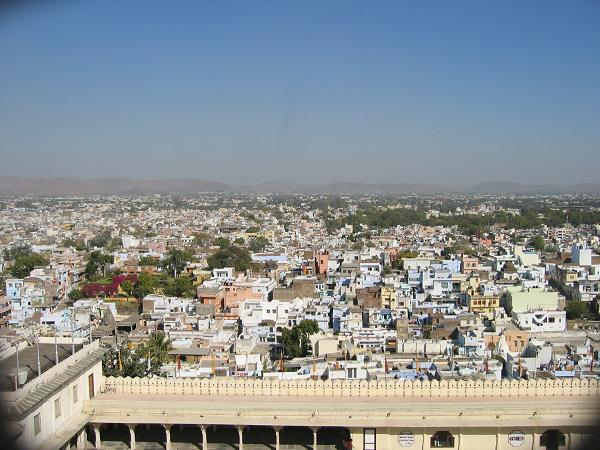
\includegraphics[width=4.8cm]{articles/Il-commence-a-faire-chaud/udaipur.jpg}
%La ville d'Udaipur.

%\hspace*{-0.65cm}
%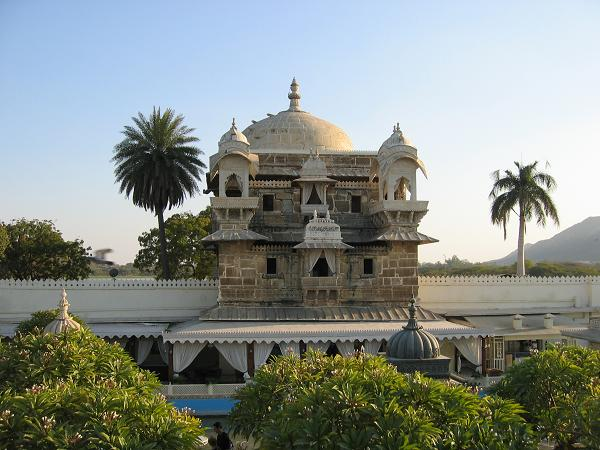
\includegraphics[width=4.8cm]{articles/Il-commence-a-faire-chaud/picchola.jpg}
%Une belle vue depuis une île du lac Pichola.

%\hspace*{-0.65cm}
%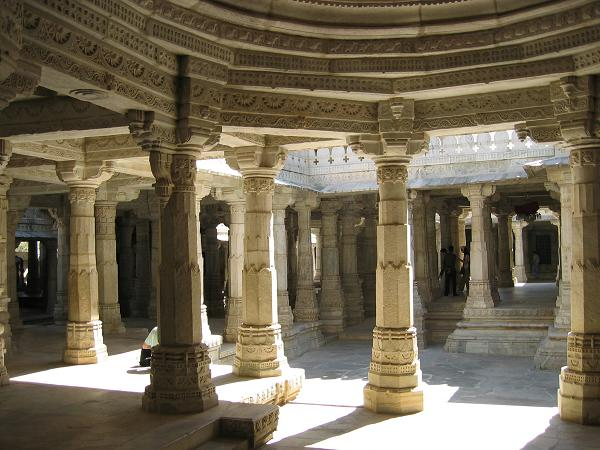
\includegraphics[width=4.8cm]{articles/Il-commence-a-faire-chaud/ranak.jpg}
%Un immense temple Jain de Ranakpur.

%\hspace*{-0.65cm}
%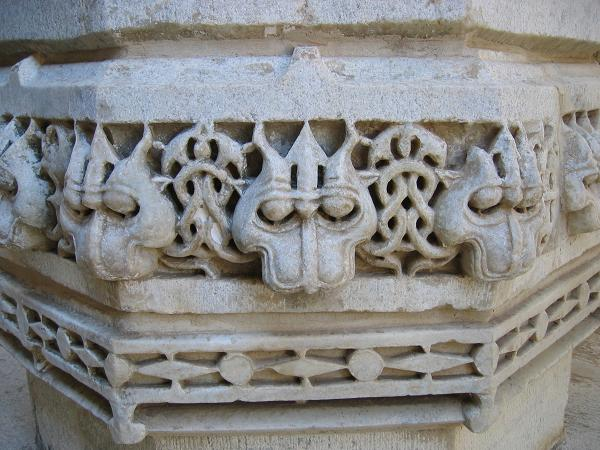
\includegraphics[width=4.8cm]{articles/Il-commence-a-faire-chaud/ranak2.jpg}
%Le détail d'un temple.

%\hspace*{-0.65cm}
%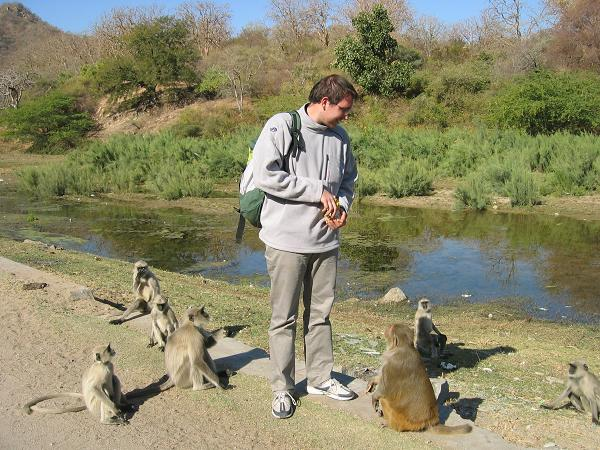
\includegraphics[width=4.8cm]{articles/Il-commence-a-faire-chaud/ranak3.jpg}
%Etienne nourissant les singes.

%\hspace*{-0.65cm}
%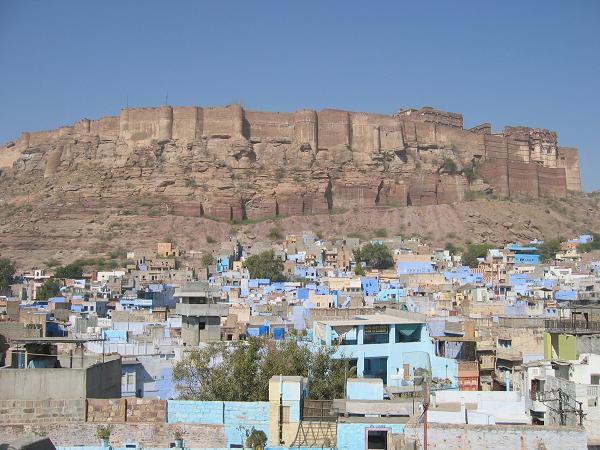
\includegraphics[width=4.8cm]{articles/Il-commence-a-faire-chaud/ranak4.jpg}
%La vue depuis la terrasse de notre guest house de Jodhpur.

Allez, parce que vous êtes sages, vous avez le droit à une video bonus.

\end{multicols}

\bigskip
\textbf{\textsc{Commentaires}}

\medskip
Titou a écrit le 18 fév. 2008 :
\begin{displayquote}
Ra vous nouys faites rever meme sans les images. Je comprend ce que vous ressentez car je l'ai ressenti ici aussi meme si l'univers est completement different. C'est toujours tres dur de transmettre ce que l'on ressent et que l'on voit parfois tellement c'est beau. Ce qui prouve que notre monde regorge de choses magnifiques dont on ne soupsconne parfois pas l'existence\dots Profitez en toujours a fond, faites de ce sejour un souvenir memorable et on se revoit dans peu de temps. Faites gaffe a vous et a plus. Biz.
\end{displayquote}

\medskip
Lydie a écrit le 19 fév. 2008 :
\begin{displayquote}
Ahlala, vos paroles sont encore plus belles que les images. On se plonge avec "extase" à travers vos écrits !!!
Profitez-bien de vos derniers jours !!! Et j'attends de tes nouvelles ma poulette. Bisous.
\end{displayquote}

\medskip
Zan a écrit le 19 fév. 2008 :
\begin{displayquote}
Hébé, ça dépayse de la Franche-Comté\dots
Vous devez vraiment en avoir plein les yeux et les oreilles tous les jours (et ptet plein le c*l aussi des singes :D)!
Continuez de nous faire rêver avec ces photos, elles sont vraiment magnifiques!
@ bientôt!
\end{displayquote}

\medskip
Peggy a écrit le 20 fév. 2008 :
\begin{displayquote}
Etienne qui essaie d'apprendre aux singes les règles de bonnes conduites\dots j'adore!
\end{displayquote}

\medskip
Poun's a écrit le 20 fév. 2008 :
\begin{displayquote}
Salut vous deux, Bon, si vous continuez, on va affréter un avion pour vous rejoindre,,,,
La météo, toujours pas de nuages? On a l'impression qu'il ne fait pas toujours très chaud là-bas, Vous n'avz pas froid?
Continuez les photos, même si elles ne passent pas toutes, et surtout mettez-en plein votre tête pour nous raconter tout ça,
Félicitations au nouveau tonton, et surtout à la maman et au papa,
Ca tombe bien, je travaille à Besançon Vendredi, on va fêter ça!
A bientôt,
\end{displayquote}

\medskip
Tatid a écrit le 21 fév. 2008 :
\begin{displayquote}
J'ai toujours pas le net à l'appart, mais vu que j'ai pas grand chose à faire en stage, j'en profite pour ratrapper ma lecture de blogs (j'ai lu l'intégral de "Fab aux USA" en 2 jours ^^) !
Vos photos sont vraiment superbes, c'est dingue le changement de culture par rapport à la notre, ça doit être vraiment enrichissant un voyage comme ça, puisqu'on est plus du tout dans la culture occidentale quoi ! Les monuments sont aussi impressionnants de beauté ! En tous cas, vous n'avez pas l'air triste (c'est le moins qu'on puisse dire !) et vous avez l'air d'en avoir profité au maximum, c'est génial !
Dis Dud, tu t'es fait des potes singes ? T'en ramène un nan ?! ^^
\end{displayquote}

\medskip
Etienne a écrit le 21 fév. 2008 :
\begin{displayquote}
Alors question meteo ca commence a chauffer. On a deja du avoir du 30 degres je pense. Merci bien pour les felicitation, je transmettrais avec grand plaisir a ma soeurette car elle ne doit plus trop avoir le temps de venir lire ce blog a mon avis\dots
Bernard, a vendredi ;-)
Tatid, on m'a meme propose de m'en vendre un a Agra, le mec rigolais devant ma tete de tourist a regarder le singe sur le toit de sa shop "You want it ? i give you for 100 Rs".
Continuez a nous ecrire comme ca, ca fait tres plaisir de voir que notre voyage est suivi. C est a chaque fois le suspense quand on va sur internet. A bientot.
\end{displayquote}

\medskip
Soeurette\dots a écrit le 21 fév. 2008 :
\begin{displayquote}
Comment ça j'ai ps le temps de vous lire\dots !!! je suis là\dots bon d'accord, je suis pas venu depuis un bon bout de temps, mais je ratrape mon retard ce soir pendant que Lucie dort\dots
Ce n'est pas l'endrois, mais j'en profits pour dire à tout ceux  qui me lirons que l'acouchement à été un peu dur, mais tout va bien maintenant. Ca fais du bien d'ètre chez sois\dots et Lucie à l'aire de se plaire chez elle\dots
Maintenant que j'ai parler de moi, j'espère que vous reviendrez de ce voyage plein de bons souvenir dans la tête\dots j'imagine que à peine rentré, vous allez avoir envie de repartir visiter le monde ?
Aller, continuez bien, à mardi prochain.
Bisou
Cécile la soeurette\dots
\end{displayquote}

\medskip
Gerien a écrit le 22 fév. 2008 :
\begin{displayquote}
Alors la grande question de la pause café de ce matin à l'alstom c'est :
Est ce que dud c'est fait bouffé la main par un singe (surtout le gros là à la fin) ?
Allez, bonne fin de voyage les gens ;o)
\end{displayquote}

\medskip
Etienne a écrit le 23 fév. 2008 :
\begin{displayquote}
Hehe\dots je voit que ca bosse dur dans les bureau d'Alstom\dots
Les singes etaient trop content qu'on leur donne a manger pour etre agressifs, en fait ils doivent avoir l'habitude car il y a beaucoup de passage la ou on etait. Mais par contre on en a deja vu flanquer la frousse a une touriste jusqu'a ce qu'elle lache la pomme qu'elle etait en train de manger, et ca c'est assez impressionnant a voir, on doit rapidement se dire qu'une pomme ne vaut pas une morsure de singe.
\end{displayquote}

\medskip
Poun's a écrit le 23 fév. 2008 :
\begin{displayquote}
Salut à vous. N'oubliez pas de prendre des pommes, si ça peut vous sauver une main\dots
Pensez à ma commande : une vache sacrée, un singe, 1 l'd'eau du Gange et si vous avez un peu de place dans vos bagages, un éléphant me serait très utile.
A bientôt pour vos nouvelles aventures, j'espère que vous ne mourez pas de chaud.
\end{displayquote}

\medskip
Gerien a écrit le 24 fév. 2008 :
\begin{displayquote}
Moi, ce que je commanderais prendrais moins de place\dots
:)
\end{displayquote}

\vfill


\pagebreak\section{Sniff}

Date: 25/02/2008

\begin{multicols}{2}

Et oui, ce n'est pas sans émotion que nous écrivons notre dernier post depuis l'Inde.

De retour à Delhi depuis 2 jours pour faire des achats, nous avons profité à fond de nos derniers moments et surtout de notre dernier rickshaw (45 minutes pour faire 3km quand même). Dernier banana lassi, une boisson au yaourt bien sympa, dernier repas Indien, dernière fanfare dans la rue, derniers feux d'artifice au dessus des toits, dernier bazar coloré...

Merci beaucoup à tous, ceux qui laissent des commentaires mais aussi ceux qui n'osent pas, de nous avoir lu tout au long de ce périple. Ca nous a fait bien plaisir de partager tout ça avec vous.

A bientôt pour un article récapitulatif de conseils de voyages pour l'Inde.

Cécile et Etienne.

\end{multicols}

\bigskip
\textbf{\textsc{Commentaires}}

\medskip
Sylvie a écrit le 25 fév. 2008 :
\begin{displayquote}
Du brahmane à l'intouchable le système des castes est il visible encore aux yeux du voyageur ?

Avez vous été à Bénarès ville sainte au bord du Gange ?	Je pense que vous avez énormément de merveilleuses images dans votre tete .Si de belles photos sont mises sur le blog je serai ravie car je n'ai pu en ouvrir que quelques unes .Etienne félicitations pour tes examens et va vite voir la puce .A bientôt sylvie
\end{displayquote}

\medskip
Catherine a écrit le 26 fév. 2008 :
\begin{displayquote}
Ca va faire du bien de vous revoir même s'il me faudra apprendre à me passer de vos nouvelles, car je n'en ai jamais autant quand moins de kilomètres nous séparent et qu'il n'y a pas toutes ces émotions à nous faire partager.
         Très bon retour et à bientôt. (à mercredi matin pour Cécile)
\end{displayquote}

\medskip
Jaco a écrit le 26 fév. 2008 :
\begin{displayquote}
Erf, déjà fini votre trip :S C'est triste, j'vais plus pouvoir voyager depuis le bureau.
J'espère que toi Etienne tu foutras le camp bientôt ^^
Et Cécile bon stage :D Fini les voyages, retour sur Terre !
See ya
\end{displayquote}

\medskip
Tatid a écrit le 26 fév. 2008 :
\begin{displayquote}
Merci pour ce petit blog et pour toutes ces photos ! Vous devez avoir des souvenirs plein la tête !
Bon retour en France pour Céc, et pour Dud, bah je suivrai tes futures aventures :)
A+, j'ai un peu de taff (sisi pour une fois !)
\end{displayquote}

\medskip
Titou a écrit le 26 fév. 2008 :
\begin{displayquote}
Mrd genre Tatid travaille\dots ça se saurait :p
Désolé pour le retard mais j'ai eu quelques petits soucis de transport pour mon retour au pays mais je vais quand même vous dire que je suis bien content que votre séjour vous ai ravi ! Et je pense que c'est un faible mot pour décrire ce que vous ressentez. Bon voyage pour le retour et on se voit très bientôt !
A plus les jeunes, Biz
\end{displayquote}

\medskip
Sam a écrit le 27 fév. 2008 :
\begin{displayquote}
Bon retour à vous, profitez de vos derniers moments là bas pour graver de belles images dans vos têtes et garder plein de souvenirs !
- Sam
\end{displayquote}

\medskip
Lydie a écrit le 28 fév. 2008 :
\begin{displayquote}
sniff sniff, mes moments de divertissement derrière mon PC sont finis !!!
J'espère que le retour n'a pas été trop dur !
Bon courage pour ton stage ma poulette
A très bientôt je l'espère
Gros Bisous
\end{displayquote}

\medskip
Ange\_blond a écrit le 29 fév. 2008 :
\begin{displayquote}
Fin des aventures\dots ben oui faut bien que ça s'arrête un jour quand même\dots
Ma petite Cécile, ça ne t'as meme pas manqué des petits pointeurs et des pixels/vertexs qui se balladent jamais là où il faudrait ?
J'espère bien que non, histoire que tu ait bien profité de tes vacances\dots
@+ missryxie
\end{displayquote}

\medskip
PoPoL a écrit le 12 mars 2008 :
\begin{displayquote}
Merveilleux voyage ! Bonne continuation à vous deux, et au plaisir de vous revoir un de ces 4 !
\end{displayquote}



%\chapter{La vie curieuse avant la vie active}
%\section{C'est bientôt reparti}

26 mars 2008

\begin{multicols}{2}

Ca y est, c'est les derniers préparatifs pour repartir en Asie.

Direction l'Indonésie pour faire un tour de voilier, en fait c'est un peu plus qu'un tour. Nous allons partir avec Patrick, le propriétaire du bateau, de Bali où il est actuellement pour remonter en direction de la Thaïlande, en passant par Singapour et la Malaisie.

Je vous laisse regarder sur une carte ce que ça donne : nous allons naviguer en Indonésie en passant par les îles de Bali, Bornéo, Java, puis le détroit de Malacca. Puis nous passerons à Singapour et en Malaisie du coté Ouest, nous remonterons jusqu'à la Thaïlande, à Phuket.

\smallbreak
\hspace*{-0.65cm}
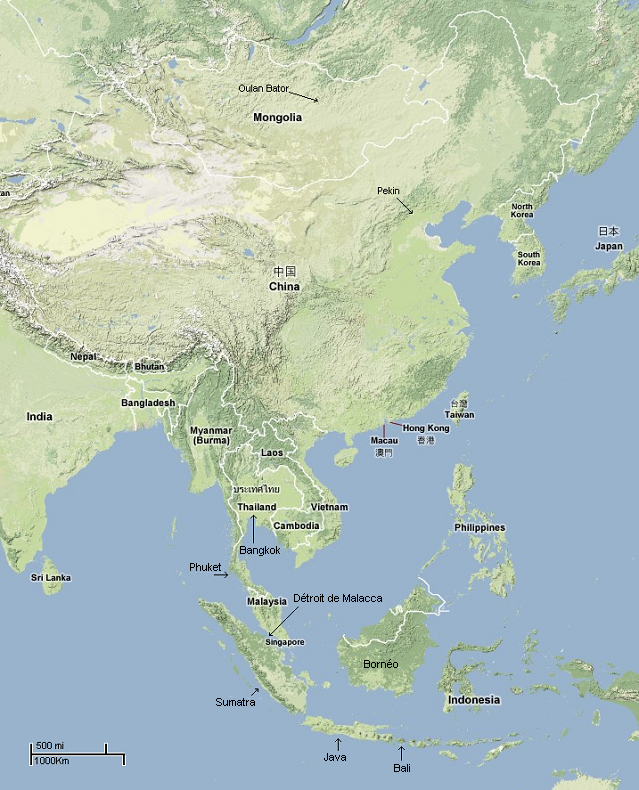
\includegraphics[width=5cm]{articles/C-est-bientot-reparti/trip.png}
%Le trip prévu.
\smallbreak

La suite est moins organisée, je reprends mon sac à Phuket, direction Bangkok pour aller voir une amie de mes parents qui s'appelle devinez comment... ? Cécile bien sûr... Après Bangkok direction le Laos pour aller en Chine... mais peut être, sans doute, un passage par le Vietnam (Gad je compte sur toi).

Le but final est d'aller en direction de Pekin pour prendre le train trans-mongolien jusqu'à Oulan Bator, capitale de la Mongolie.

Mais rien n'est moins sûr que j'arrive jusque là, en effet je ne fais pas une course, et j'ai quelques contacts de personnes à aller voir (Cécile à Bangkok, Stéphane vers Macao), d'autre personnes avec qui je ferai sûrement une partie du trajet (Dayana, Gad, ... à confirmer).

Une contrainte : être rentré pour mi juillet car je commencerai ensuite un stage à Paris pour terminer mes études.

Voila, je pars mardi 1er avril et d'ici là je termine quelques trucs et je fais mon sac.

Au plaisir de lire vos commentaires durant ce voyage, j'essaierai de vous montrer de belles photos et faire de bons récits. A bientôt.

\end{multicols}

\bigskip
\textbf{\textsc{Commentaires}}

\medskip
Jaco a écrit le 27 mars 2008 :
\begin{displayquote}
Et bien bon vent mon ptit Dud et fait attention à la chaleur ;) Si t'en as trop ramène en un peu en Alsace !
Ciao et à la prochaine !
\end{displayquote}

\medskip
Cécile, qui fait pas le voyage a écrit le 28 mars 2008 :
\begin{displayquote}
Ah là là, plein de belles choses en perspectives, tu vas t'amuser comme un p'tit fou! Comme d'hab, ouvre grand tes mirettes, profite bien du bateau, et reviens-nous en pleine forme!
Je te fais des gros bisous.
\end{displayquote}

\medskip
Tatid a écrit le 31 mars 2008 :
\begin{displayquote}
Bon voyage Dud ! Profites en bien\dots Je suivrai tes aventures sur ton blog\dots Par contre, en tant que bon GI, tu pourrais nous faire un petit flux RSS là :-P
\end{displayquote}

\medskip
Isa a écrit le 31 mars 2008 :
\begin{displayquote}
Salut dud,
Profites en bien et n'oublie pas de nous faire partager de belles photos ça donnera envie d'y aller!
Gros bisous\dots
\end{displayquote}

\medskip
Etienne a écrit le 2 avril 2008 :
\begin{displayquote}
Ne vous inquiétez pas pour les photos, cette fois j'ai assuré le coup si j'ai des problèmes Mac se chargera de sauvegarder les photos en lieu sûr depuis une connexion internet digne de ce nom.
Ca y est c'est parti, je suis en transit à l'aéroport de Singapour, super classe !!!
A bientôt.
\end{displayquote}

\medskip
Titou a écrit le 2 avril 2008 :
\begin{displayquote}
Salut mon pti Dud ! Content de voir que la première partie de ton voyage s'est bien passée ! Profites en à fond et fais nous baver avec tes futures photos !
As we say out there, take care, enjoy and have fun !
A plus mon pote\dots
\end{displayquote}

\vfill


%\pagebreak\section{Fiche de l'Indonésie}

Date: 30/03/2008

\begin{multicols}{2}
\hspace*{-0.65cm}
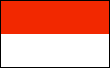
\includegraphics[width=4.8cm]{articles/Fiche-de-l-indonesie/drapeauindonesie.png}
Drapeau de l'Indonésie

\subsection{Situation}
\subsubsection{Présentation générale}

En Asie du Sud-Est, entre océan Indien et Océan Pacifique, le plus grand archipel du monde traverse trois fuseaux horaires et s'étend sur plus de 5000 km d'Est en Ouest et 2000 km du Nord au Sud. Des 13.000 îles qui le composent, 6000 sont inhabitées. Les îles de la Sonde (Sumatra la plus vaste, Java, Bali, Lombok, Sumbawa, Sumba, Flores, la moitié Ouest de Timor), la plus grande partie de l'île de Bornéo (Kalimantan), l'île de Célèbes (Sulawesi), l'archipel des Moluques et Irian Jaya depuis 1963 (partie Ouest de l'île de Papouasie Nouvelle-Guinée) représentent l'essentiel de sa superficie (1.919.000 kilomètres carrée, soit trois fois et demie la France).

Les frontières maritimes de l'Indonésie sont avec l'Inde, la Malaisie, Singapour, la Thaïlande, le Vietnam, les Philippines et l'Australie. L'Indonésie partage deux frontières terrestres, 1782 km avec la Malaisie sur l'île de Bornéo et 820 km avec la Papouasie Nouvelle-Guinée sur Irian Jaya, à l'Est de l'archipel.

Chevauchant la ligne de l'équateur, l'Indonésie est également une vaste zone de volcans, la "ceinture de feu", où culmine le sommet enneigé de Puncak Jaya (5030 m) sur Irian Jaya. Soixante dix à quatre vingt d'entre eux sont encore en activité.

Forêts tropicales, savanes, marécages, montagnes et volcans contribuent à faire de l'Indonésie un pays exceptionnellement diversifié.

\subsection{Population}

Avec une population estimée à 206 millions d'habitants en 2001, l'Indonésie est le quatrième pays de la planète après la Chine, l'Inde et les Etats-Unis. Le taux de croissance annuel a baissé de façon significative au cours de la dernière décennie passant d'un taux de croissance annuel moyen de 1,97% entre 1980 et 1990 à 1,35% entre 1990 et 2000. Cette baisse est en partie le résultat de campagnes gouvernementales prônant l'utilisation de moyens de contraception.

La densité présente de très fortes disparités avec un rapport de 1 à 120 selon les îles ; Java compte à elle seule près de 60% de la population totale de l'Indonésie (ce qui lui donne une densité de 946 hab/km², comparée à une densité moyenne de 106 hab/km² pour l'Indonésie) et englobe les trois premières villes du pays (Jakarta, Surabaya et Bandung) ; Irian Jaya abrite à peine 1% de la population. Les transmigrations du 20ème siècle, devant réduire le surpeuplement de Java avec un programme de colonisation agricole des autres îles, se traduisent aujourd'hui par des difficultés de cohabitation.

Un peu plus de la moitié de la population est âgée de moins de 24 ans et la population active est constituée de 99 millions de personnes (chiffres de 1999). Une impressionnante diversité ethnique de plus de 300 groupes différents, non prise en compte dans les statistiques, donne à penser que tous les peuples d'Asie sont représentés en Indonésie.

|                                      |     INDONESIE   |    FRANCE    |
| ------------------------------------ |: -------------: | -----------: |
|Population                            |     206 millions| 59,2 millions|
|Densité                               |      \SI{106}{hab.km^2}|   \SI{108}{hab.km^2}|
|Accroissement naturel de la population|             1,35|           0,4|
|Indice de fécondité                   |             2,58|           1,8|
|Espérance de vie                      |        68,27 ans|      78,5 ans|
|Urbanisation                          |             41 %|        75,6 %|

\subsection{Climat}

L'Indonésie est l'un des pays les plus chauds et humides de la planète. Selon les îles le climat est soit tropical, soit équatorial. La zone équatoriale (Sumatra, Bornéo, Célèbes, Irian Jaya) se caractérise par un climat très humide et ne connaît qu'une très courte saison sèche. Dans la zone tropicale (Java, Bali, petites îles de la Sonde), la saison humide alterne avec une longue saison sèche (six mois environ). Dans les petites îles de la Sonde, le climat présente même un caractère semi-aride.

L'archipel connaît deux moussons, l'une de novembre à mars, accompagnée de fortes pluies, constitue la saison la plus humide, et l'autre, de juin à octobre. Sur l'année, la température reste relativement élevée, la moyenne minimale se situant à 22/23 degrés C en saison des pluies et la moyenne maximale à 33/34 degrés C. Il n'y a pas de saisons définies. La moyenne des précipitations oscille entre 1780 mm et 3175 mm par an mais certaines régions peuvent recevoir jusqu'à 4 mètres d'eau (5 mètres dans les régions montagneuses de Kalimatan).

\subsection{Villes principales}
\subsubsection{Jakarta}

Jakarta est la capitale de l'Indonésie et la ville la plus peuplée du Sud-Est asiatique (mégalopole de 18 millions d'habitants avec ses banlieues). Elle est située sur la côte Nord-Ouest de Java, implantée sur les deux rives de l'éstuaire de la rivière Tjiliwung. Jakarta est le grand centre industriel du pays. La zone industrielle de Pulo Gadung regroupe les principales industries de Java (papier, métallurgie, automobile, tanneries, textile, produits chimiques, alimentation, électronique). Jakarta absorbe 80% des investissements étrangers.

En 1619, la Compagnie hollandaise des Indes orientales établit un comptoir commercial à Jayakerta et rebaptise la ville Batavia, future capitale des Indes néerlandaises. C'est lors de l'occupation japonaise durant la Seconde guerre mondiale que Batavia reprit son nom indonésien. Nombre de bâtiments coloniaux, comme les entrepôts de la VOC, sont transformés en musée. L'aéroport est distant de 30 km.

\subsubsection{Surabaya}

Surabaya est la capitale de la province orientale de Java, située à l'embouchure du fleuve Kali Mas sur le littoral nord est de Java. C'est la deuxième plus grande ville (et port) d'Indonésie après Jakarta (4 millions d'habitants). Surabaya est avant tout un centre industriel où l'on trouve aciéries, raffineries de sucre et de pétrole, scieries, industries alimentaire et de fabrication de machines, de production de verre, de textile, cimenteries ainsi qu'une base navale. La ville est le siège de l'université d'Airlangga (1954), de l'université Petra Christian (1965) et de l'Institut technologique de Surabaya (1960). Jusqu'en 1939, Surabaya fut la plus importante base navale des Indes orientales néerlandaises.

\subsubsection{Bandung}

Bandung est la capitale de la province de Java Barat. Elle compte plus de deux millions d'habitants. Bandung est située à environ 180 km au sud est de Jakarta et sur un plateau à 715 m d'altitude. C'est un grand centre industriel et une capitale culturelle.

Ses usines sont spécialisées dans la fabrication de textiles, de teintures, de produits chimiques, dans les constructions mécaniques et la céramique. La ville abrite le prestigieux Institut de Technologie de Bandung (1955), l'université d'Etat de Pajajaran (1957) et l'université catholique de Parahyangan (1955). La ville est souvent présentée comme le centre culturel du pays sundanais.

Des colons hollandais fondèrent Bandung en 1810. La ville devient le siège administratif et militaire des Indes orientales hollandaises. L'industrialisation s'y developpa à la fin du 19ème siècle avec l'introduction du chemin de fer dans l'archipel.

\subsubsection{Medan}

Medan est la capitale de la province de Sumatra-Nord et la première ville sur l'île de Sumatra (2 millions d'habitants). Elle est située sur les confluents des rivières Deli et Babura, près de Belawan (le port de Medan sur le détroit de Malacca). Les industries sont centrées sur l'exploitation des ressources de la région (agroalimentaires, torréfaction du café, thé et industries textiles).

Medan est aussi une importante ville commerciale pour l'hévéa, le tabac, le thé, l'huile de palme et le café. Elle accueille l'université du Sumatra-du-Nord (1952), l'université islamique du Sumatra-du-Nord (1952), un institut de recherche sur le tabac, le palais et la résidence du sultan de Déli, une grande mosquée, le plus grand temple chinois d'Indonésie. La ville se développa après 1870 et connut une forte expansion industrielle dans les années 1940-1950.

\subsubsection{Semarang}

Capitale de la province de Java Tengah à l'embouchure du Semarang sur la côte nord de Java. La ville est reliée par des navettes aériennes quotidiennes aux principales cités indonésiennes. Semarang est un port maritime (pêche, exportation de sucre, coprah, tabac, café et caoutchouc), centre commercial et industriel (construction navale, textile, fabrication d'équipements électriques et de matériel ferroviaire). Sa population de 1,4 million d'habitants compte une importante communauté chinoise. Le vieux quartier de la ville comprend un bel ensemble de bâtiments datant de l'époque coloniale et à 5 km du centre se trouve le temple Sam Po Kong (15ème siècle), lieu de pèlerinage important pour les musulmans et les Chinois.

\subsubsection{Ujung Pandang/Makassar}

Ujung Pandang est la capitale de la province de Sulawesi Selantan au sud-est de l'île des Célèbes. Elle compte 1 million d'habitants. C'est la première ville et le plus grand port de Célèbes. Le site fut exploré, puis colonisé par les Portugais en 1512. Les Hollandais s'en emparent au début du 17ème siècle. Dans les années 1970 on adopta à nouveau son ancien nom (Makassar). Ellle est un important carrefour maritime et aérien entre l'est et l'ouest de l'archipel indonésien, en tant que pôle commercial et point de déchargement des produits acheminés d'une île à l'autre de l'Indonésie. La ville est aussi un centre industriel (produits alimentaires, textiles, papeterie et matériaux de construction). Dans la ville se trouvent l'université de Hasanuddin (1956), un musée de l'artisanat local et le fort Vredenburg.

\subsubsection{Yogyakarta}

La ville est située au centre de l'île de Java, au pied du volcan Merapi. Elle compte un peu plus de 500 000 habitants. Yogyakarta était aux 16ème et 17ème siècle le siège du puissant empire javanais de Mataram. Yogyakarta est née en 1755 après la division de Mataram en deux sultanats, celui de Yogyakarta et celui de Surakarta. Elle était possession néerlandaise avant la Seconde guerre mondiale. A la suite de la proclamation d'indépendance en 1945, le sultanat fut intégré à la République indonésienne et Yogyakarta en devint la capitale jusqu'en 1950 (date à laquelle elle fut remplacée par Jakarta). La ville est située au coeur d'une région fertile produisant canne à sucre, riz et tabac. Alliant le dynamisme de la jeunesse d'une ville universitaire et la tradition vivante d'une capitale de la culture javanaise, complexe et raffinée, elle est devenue une destination touristique majeure permettant d'accéder notamment au temple bouddhiste de Borobudur (8ème siècle).

\end{multicols}

\bigskip
\textbf{\textsc{Commentaires}}



%\pagebreak\section{Arrivé sur Bali}

Date: 07/04/2008

\begin{multicols}{2}

Salut tout le monde !!! Bon alors, autant vous le dire tout de suite, vu les photos qui sont dans cet article, vous allez me détester quand vous les aurez vues... enfin disons qu'il y a de fortes chances... Arrivé mercredi, sans aucun souci durant le trajet, Patrick est venu me chercher à l'aéroport pour aller au bateau, joli canot de 13m50, bien équipé pour la navigation, spacieux. Nous sommes allés faire un petit tour à Kuta, coin le plus touristique de Bali, Plage très appréciée des surfers du monde entier. En fait j'ai adoré le passage ombragé qui longe la route et la plage, où une multitude des petits vendeurs proposent location de planche de surf, boissons fraîches et massages, vraiment très tentant.

\hspace*{-0.65cm}
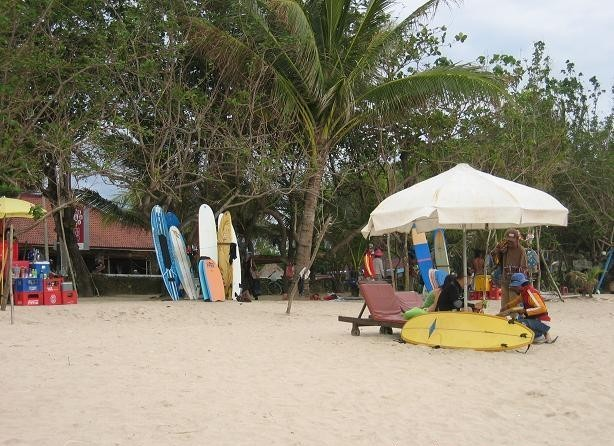
\includegraphics[width=4.8cm]{articles/Arrivee-sur-bali/1207567562ikVd.jpg}
Plage de Kuta

Sylvie, une amie de Patrick, est arrivée avec sa fille Tamara le soir, pendant que j'étais dans les bras de Morphée, décalage horaire oblige. Nous somme partis jeudi et revenus samedi matin pour faire un tour dans Bali, en s'arrêtant dans des petits hôtels bien sympathiques (c'est un euphémisme) avec vue sur mer, cocotiers, piscines, eau à 30 degrés quand elle est froide...

\hspace*{-0.65cm}
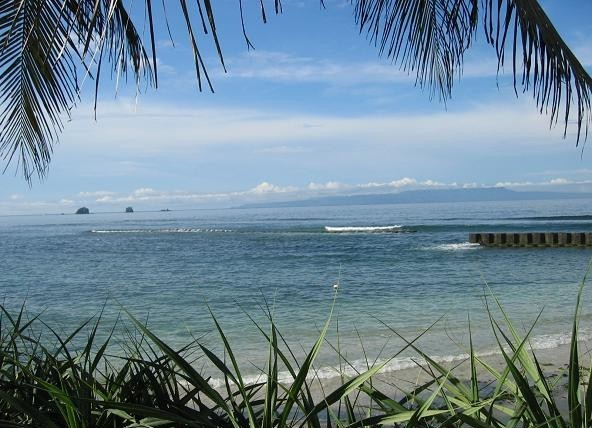
\includegraphics[width=4.8cm]{articles/Arrivee-sur-bali/1207567561DqJk.jpg}
La mer

\hspace*{-0.65cm}
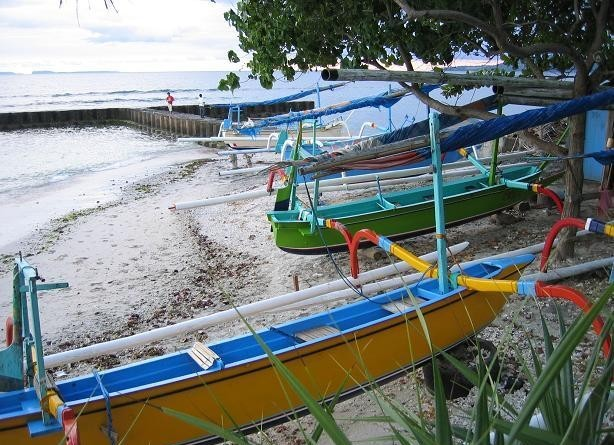
\includegraphics[width=4.8cm]{articles/Arrivee-sur-bali/1207567564x5vI.jpg}
Bateau de pêche traditionnels

\hspace*{-0.65cm}
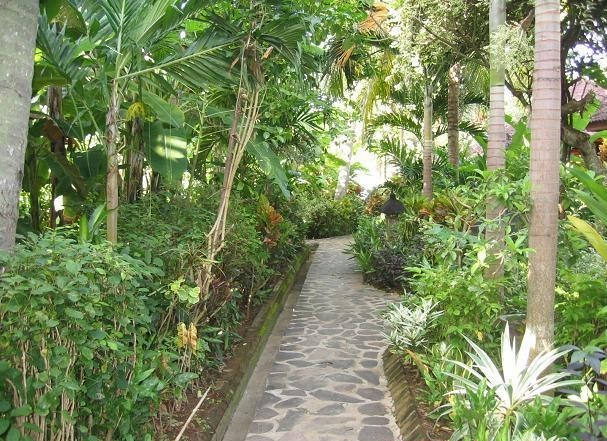
\includegraphics[width=4.8cm]{articles/Arrivee-sur-bali/120756756426sq.jpg}
L'allée d'un hôtel

\hspace*{-0.65cm}
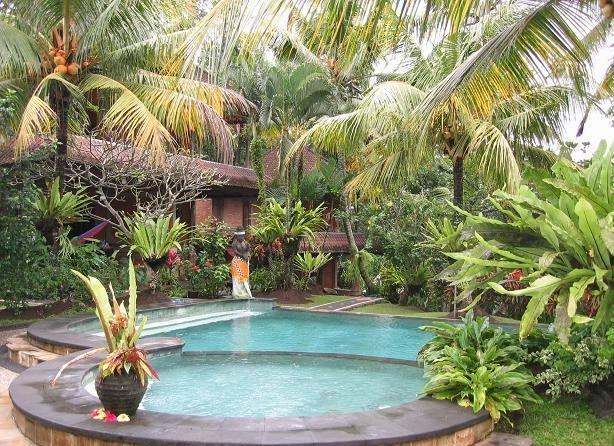
\includegraphics[width=4.8cm]{articles/Arrivee-sur-bali/1207567563njCA.jpg}
Ze piscine

La capitale de l'île est Denpasar, ville qui grouille de partout, sans gros interêt à ce que l'on m'a dit, j'irais voir quand même... L'aéroport est à Kuta, juste au Sud de Denpasar, ville beaucoup plus jolie... et touristique. En ce qui me concerne, le bateau est à la Marina de Benoa, juste à l'Est de Kuta. Je connaissais deja un peu l'artisanat de Bali, les balinais font de magnifiques objets de déco, des tissus, des sculptures, on en voit partout. Ici une photo prise au bord de la route dans un petit village

\hspace*{-0.65cm}
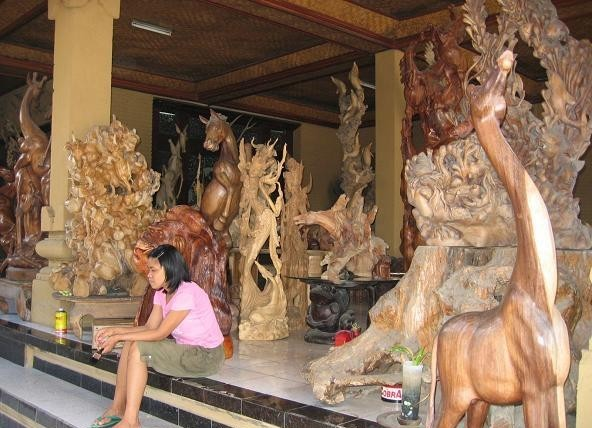
\includegraphics[width=4.8cm]{articles/Arrivee-sur-bali/1207567562ISpn.jpg}
Sculptures en bois

Dans les jours qui suivent je vais louer un scooter pour faire un tour complet de l'île, essayer d'aller voir un pote de Patrick, Indonésien, plus au Nord dans l'île, monter sur le plus gros volcan, me perdre dans les rizières, enfin pas trop de plans a l'avance, il est très facile de se loger ici, les gens sont aussi sympa qu'en Inde, et bizarrement l'immense majorité des personnes que l'on voit ont entre 20 et 25 ans.

A bientôt.

\end{multicols}

%\pagebreak\section{Round trip in Bali}

Date: 14/04/2008

\begin{multicols}{2}

Oulala... que de choses a dire...

Je vous ai laissés à la fin de ma première semaine à Bali. Ma deuxième semaine à été très mouvementée, car j'ai loué un scooter pour faire un tour de l'ile, en 4 jours.

Me voila donc parti sur les routes, avec pour seule carte un plan de l'ile qui tiendrais presque sur une seule main, sur laquelle figure les grandes routes, pour les reste, la discussion avec les gens m'a bien suffit à m'orienter.

Alors premiere precision : parlons de la circulation ici... Nous vous avions parlé avec Cécile de la circulation en Inde, je n'aurais jamais loué une scooter en Inde, trop dangereux pour un novice. Ici c'est différent... quoi que... Les intersections sont respectées, les feux aussi, mais par contre il faut savoir qu'il y a réellement deux types de circulations qui cohabitent ici : les voitures qui font ce qu'elle peuvent pour respecter le code de la route, ce qui ne les empêchent pas de s'arrêter en plein virage et au milieu de la route sur ce que l'on appelerait une route départementale. Et les 2 roues, qui font ce qu'ils veulent : On peut doubler par la gauche, par la droite, slalomer, rouler à contre sens... don't worry, be happy. De temps en temps ca a du bon d'être en deux roues...

Mais que fait la police !!! Réponse : elle encaisse les backchiches. On a beaucoup plus de chances de se faire arrêter ici quand on est "western" (blanc) que quand on est Indonésien. Pourquoi ? Parce qu'on est plus solvable bien sûr... La majorité du temps le seul et unique but du policier qui vous arrête est que vous lui donniez un billet, on peut rouler sans permis ici, du moment qu'on a 50.000 Rp en poche. Quand je parle de contrôle je ne dis pas ça en l'air, je me suis fait contrôlé trois fois ce soir même sur une zone de moins de 50m de diamètre, sans éxagérer, mais je n'ai pas eu a sortir de billets, j'étais (presque) en règle.

Nous fermons la parenthèse code la route pour cette fois-ci.

\hspace*{-0.65cm}
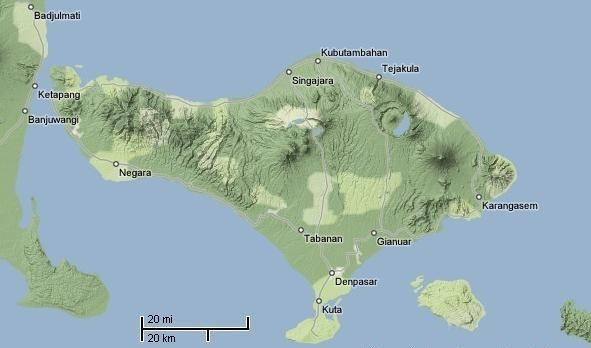
\includegraphics[width=4.8cm]{articles/Round-trip-in-bali/1208257310r6gK.jpg}
Carte de Bali


Le premier jour je suis allé dans un coin de surfers, en dessous de Tabanan, cette journée a surtout été pour moi la découverte avec la conduite indonésienne, à gauche, et son code de la route folklorique. Le soir je me suis posé à une terrasse, à discuter, je suis tombé sur des Français. Enfin quand je dis Francais, c'est d'origine, car ils voyagent tellement qu'ils n'ont jamais vu la couleur d'un euro ! La vie est belle quand on se contente de trois sous pour vivre, et ainsi voyager partout dans le monde.

Le lendemain, remontée sur Singaraja à travers de magnifiques rizières, c'est un coup à avoir un accident tellement je tournais la tete pour voir les superbes paysages qui défilaient.

\hspace*{-0.65cm}
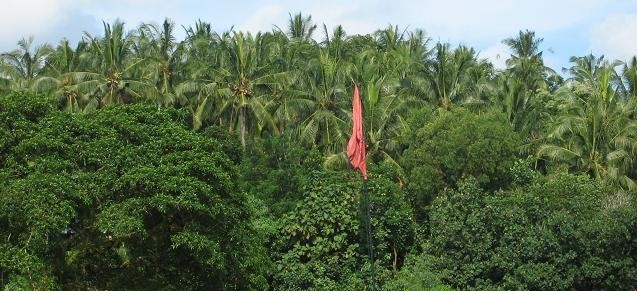
\includegraphics[width=4.8cm]{articles/Round-trip-in-bali/1208257309URc4.jpg}
Cocotiers sur la route


\hspace*{-0.65cm}
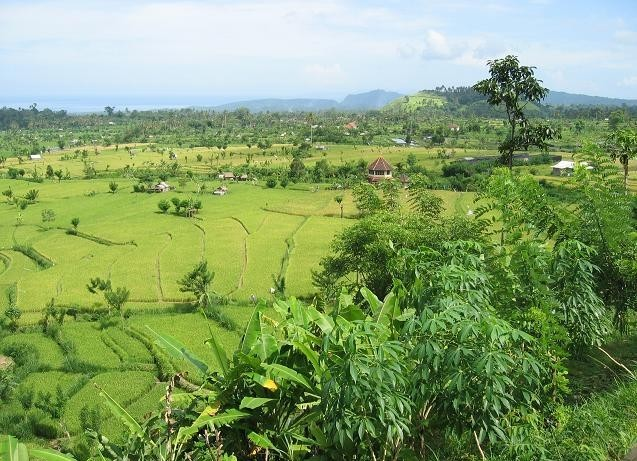
\includegraphics[width=4.8cm]{articles/Round-trip-in-bali/1208257304SP22.jpg}
Rizières


\hspace*{-0.65cm}
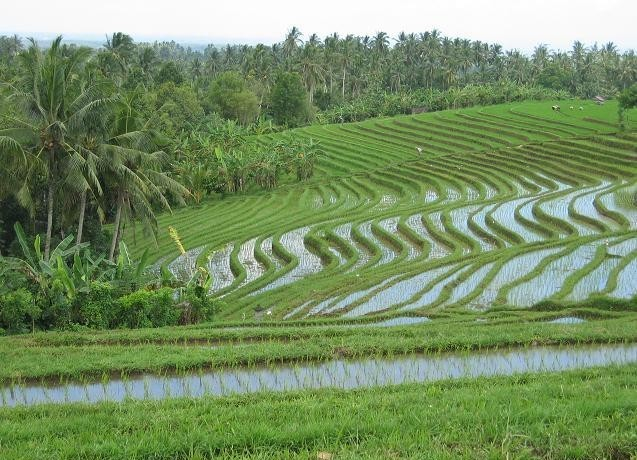
\includegraphics[width=4.8cm]{articles/Round-trip-in-bali/1208257308isJF.jpg}
D'autres rizières


\hspace*{-0.65cm}
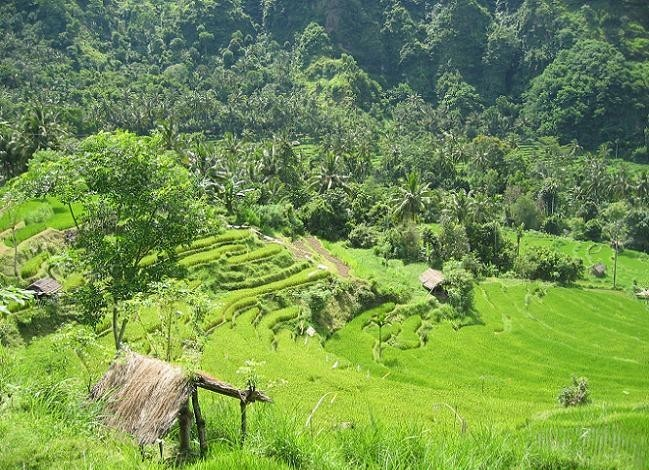
\includegraphics[width=4.8cm]{articles/Round-trip-in-bali/1208257307G9b6.jpg}
Et encore des rizières :)


Quand j'ai pris cette photo, il y avait un bruit au loin, j'ai mis du temps à comprendre qu'il s'agissait d'un homme, dans la cabane du bas, qui me faisait signe, et qui faisait du bruit pour que je le remarque. Un signe de ma part et il s'en est retourné dans sa cabane, il a du penser qu'il serait sur la photos. Les gens ici sont aussi tellement gentils que l'on a vraiment envie de leur faire plaisir.

Singaraja : pour sur ce n'est pas la meilleure étape, coin touristique si il en est, j'ai quand même réussi à me trouver un petit endroit à l'écart pour dormir, mais c'était assez difficile car, ne voulant pas paraître comme ignorant quand on leur pose une question, les gens ici vous repondront toujours une direction et une distance lorsque vous cherchez un "cheap hôtel", le tout étant apres de savoir si ce que l'on vous a dit est vrai ou pas. Il m'est arrivé que l'on me réponde alors que la personne ne parlait pas anglais, et n'avait donc pas compris la question.

Apres Singaraja, direction Seraya, au bout de la pointe de Karangasem. Je suis allé dormir chez Sales, amis de Patrick, qui m'a accueilli comme un roi, nous avons passé une super soirée avec sa famille et ses amis à boire un coup.

Sales et l'un de ses deux fils, qui a adoré les séances de guilis prodigués par mes soins.

\hspace*{-0.65cm}
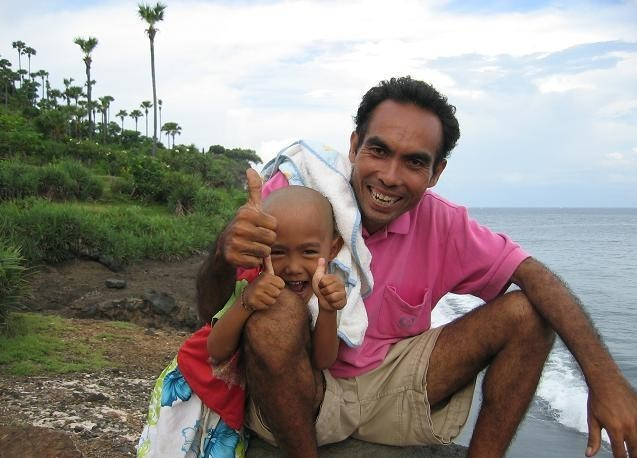
\includegraphics[width=4.8cm]{articles/Round-trip-in-bali/1208257303gr5r.jpg}
Sales et son fils Edi


Et vous savez quoi... ? j'ai eu un super petit dej le lendemain matin, une noix de coco qui était encore à 15m de haut 10 minutes avant que je boive son jus... si c'est pas la classe...

\hspace*{-0.65cm}
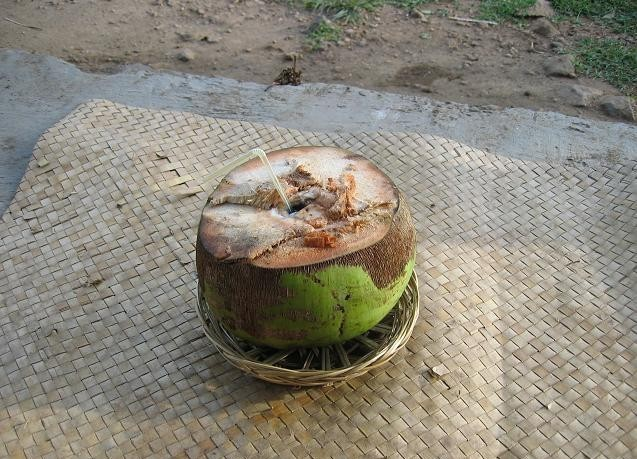
\includegraphics[width=4.8cm]{articles/Round-trip-in-bali/1208257299a93l.jpg}
Mon p'tit dej'


Je suis redescendu de Seraya avec Sales en scooter, puis, en repartant demain, nous le déposerons près de chez lui après environs 7 heures de voile.

C'est maintenant les opérations de remplissage des soutes, avec de l'eau, du carburant, et de la nourritures. Puis dire au revoir, surtout pour Patrick qui a été ici durant 7 mois. De mon coté aussi c'est un peu dur de partir, il y a déjà des personnes que j'aimerais revoir.

Direction Madura, sur l'île de Java pour les jours à venir, puis Bornéo, plus au nord. Et de Bornéo nous mettrons le cap sur Singapour, où je dois arriver avant la fin de mon visa Indonésien (fin du mois d'avril).

Voila, j'éspère que suivre mon voyage vous plaît toujours, je vous dis à très bientôt.

\end{multicols}

%\pagebreak\section{La Java bleue}

Date: 23/04/2008

\begin{multicols}{2}

Comme vous l'avez (sûrement) (pas) remarqué en lisant le titre de cet article, je viens de traverser la mer de Java, la java bleue quoi (oui ben c'est bon... après 4 jours de mer vous auriez aussi un humour minable...).

C'est avec amertume que je vous écris ces lignes, en effet j'entrais tranquillement dans le cyber café où je suis avec la ferme intention de vous faire partager mes toutes dernières videos de navigation, quand j'ai remarqué que le débit internet ici ne me permettrait jamais de vous faire voir ces magnifiques moment. Premier essai... rien. Deuxième essai... rien.

Laissez moi quand meme vous conter mes derniers jours, j'ajouterais les videos à ce texte quand je serai à Singapour.

C'est le départ, tout le monde sur le pont !!! Nous avons fait des courses, remplis les réservoirs d'eau, de fuel, tout l'avitaillement nécessaire à notre traversée pour Bornéo depuis Bali.

Ca y est, c'est parti... ça fait quelque chose de quitter cette jolie île, est ses habitants tous plus gentils les uns que les autres. Direction Seraya, pointe Nord-Est de l'île pour laisser Sales qui aura fait un petit bout de route avec nous, puis direction Madura, une île un peu au Nord de Java, voici les premières 24h passées en navigation, la première nuit, les premiers quarts. Nous jetons l'encre, à l'abris de l'île pour la deuxième nuit, puis repartons de bonne heure le lendemain (enfin de bonne heure, 8h du mat' quoi, c'est pas de notre faute on a pas entendu le coq, on était trop loin de la terre). C'est parti pour 2 jours et demi de navigation à la voile... puis au moteur, par manque de vent (c'est pas le tout mais on est pas en vacances, on a des horaires à tenir... quoi ? non ? ah bon !).

Navigation... Navigation... Ah, tient, un barracuda vient de mordre à notre ligne de traîne... miam... ça fera le repas de ce soir. Navigation... Navigation...

100h de navigation, Bornéo est en vue... enfin serait en vue si il n'y avait ce temps gris qui vient de tomber il y a 2h... et le vent qui monte... il se stabilise à 20 noeuds... parfait. Allez pour les 100h on a fait un petite video, 3 videos en fait, mais vous allez devoir patienter que je soit à Singapour pour vous les envoyer, je vous promet que ca vaut le coup d'attendre. Vous y decouvrirez entre autre l'intérieur du bateau dans lequel nous vivons.

Arrivés à Bornéo avant hier, nous posons un pied à terre, plage sympa, on cherche les pirates, on trouve pas, deçus...

Notre but maintenant est de refaire le plein de pétrol pour le bateau, puis de visiter le coin. Il parait que Bornéo est un des derniers endroits au monde où il existe des Orang Outan en liberté, on va pas manquer l'occasion d'aller leur serrer la pince, d'ailleurs c'est prévu pour demain. Je vous donnerai des nouvelles, bien sûr !

Dans l'attente de pouvoir t'envoyer mes videos, je te dis, cher lectrice, cher lecteur, à bientôt.

Etienne.

Voici enfin les videos promises. Nous commencons par le trajet entre Bali et Borneo.

%<div><object width="640" height="505"><param name="movie" value="http://www.dailymotion.com/swf/x5bijw&v3=1&related=1"></param><param name="allowFullScreen" value="true"></param><param name="allowScriptAccess" value="always"></param><embed src="http://www.dailymotion.com/swf/x5bijw&v3=1&related=1" type="application/x-shockwave-flash" width="640" height="505" allowFullScreen="true" allowScriptAccess="always"></embed></object></div>

%<div><object width="640" height="505"><param name="movie" value="http://www.dailymotion.com/swf/x5bjba&v3=1&related=1"></param><param name="allowFullScreen" value="true"></param><param name="allowScriptAccess" value="always"></param><embed src="http://www.dailymotion.com/swf/x5bjba&v3=1&related=1" type="application/x-shockwave-flash" width="640" height="505" allowFullScreen="true" allowScriptAccess="always"></embed></object></div>

Puis le trajet entre Bornéo et Singapour.

%<div><object width="640" height="505"><param name="movie" value="http://www.dailymotion.com/swf/x59cll&v3=1&related=1"></param><param name="allowFullScreen" value="true"></param><param name="allowScriptAccess" value="always"></param><embed src="http://www.dailymotion.com/swf/x59cll&v3=1&related=1" type="application/x-shockwave-flash" width="640" height="505" allowFullScreen="true" allowScriptAccess="always"></embed></object></div>

%<div><object width="640" height="505"><param name="movie" value="http://www.dailymotion.com/swf/x59o81&v3=1&related=1"></param><param name="allowFullScreen" value="true"></param><param name="allowScriptAccess" value="always"></param><embed src="http://www.dailymotion.com/swf/x59o81&v3=1&related=1" type="application/x-shockwave-flash" width="640" height="505" allowFullScreen="true" allowScriptAccess="always"></embed></object></div>

\end{multicols}

\bigskip
\textbf{\textsc{Commentaires}}

\medskip
Bobo a écrit le 25 avril 2008 :
\begin{displayquote}
Salut ma grosse ! ben ça faisait longtemps que j'était pas passé jeter un oeil, je ne suis pas déçu !
Bon tout d'abord, comme tu l'as deviné, je te hais ! ;-) on devrait pas avoir le droit de montrer les photos des autres articles à des gens qui vivent dans un endroit où ça dépasse à peine le 14 degrés C !
Bon, maintenant fait péter les vidéos, et cette fois-ci débrouilles toi pour garder toutes les photos pour nous faire une belle petite présentation de ton voyage ! ;-)
Bonne continuation mon petit salaupio ! tu sais ce qui va t'arriver quand tu reviendras !
Biz, Bobo.
\end{displayquote}

\medskip
Titou a écrit le 28 avril 2008 :
\begin{displayquote}
Yeah ti Dud !
A ba ça fait plaisir d'avoir des news et de savoir que les pirates t'ont épargné ! Mais bon fais gaffe quand même !
Je confirme ce que dit Bobo, je te hais aussi car vla la galère que c'est ici avec le boulot, le temps pourri et surtout l'UTBM :D Eclates toi bien et à très vite !
A plus mon pote !
Bisous ma poule.
\end{displayquote}

\medskip
Peggy a écrit le 1 mai 2008 :
\begin{displayquote}
Merci pour ta réponse. J'espère que tout se passe bien pour toi, on a hâte de découvrir ton séjour en image et en nouvelles anecdotes!
Prends soin de toi.
\end{displayquote}

\medskip
Pierre a écrit le 5 mai 2008 :
\begin{displayquote}
Super tes commentaires!
Promis je fais passer ton adresse à Gad.
Mais ça reste Gad !
Continue de triper (voir même fais le pour 2!) !
Sinon t'inquiètes pas pour les pirates ils sont tous en Somalie en ce moment!!!
Bonne route et à bientôt.
\end{displayquote}

\medskip
Etienne a écrit le 5 mai 2008 :
\begin{displayquote}
Ah ben tu me rassures Pierre, ça tombe bien j'avais pas prévu d'aller en Somalie, pour Gad, je suis sûr que lui parler de voyage lui fera se bouger les fesses.
Pour les commentaires, il s'agit un bête robot qui s'amuse à me pourrir mon blog, j'en suis désolé et essaie de les supprimer quand il arrivent, mais j'en ai pas toujours la possibilité.
\end{displayquote}

\medskip
Gaëlle! a écrit le 7 mai 2008 :
\begin{displayquote}
Salut mon didoum!
Ca fait plaisir de te voir! et surtout de pouvoir partager avec toi ce que tu vis sur l'eau.
Y'a pas beaucoup de vent apparament mais vous ne perdez pas votre temps pour autant: Santé à toi et à Patrick!
A la prochaine.
\end{displayquote}

\medskip
Peggy a écrit le 8 mai 2008 :
\begin{displayquote}
Trop sympas tes vidéos!
C'était vache les pieds dans l'eau car nous aussi on veuuuuuuuuuut!! on veut aussi du gateau remarque.
Par contre, je vous laisse boire le vin, toi et Pat :) SANTE!
\end{displayquote}

\medskip
Pierre a écrit le 8 mai 2008 :
\begin{displayquote}
Hey!
Gad m'a répondu. Il a dû t'envoyer un message...
Top les vidéos, c'est une super idée... Fais en plus!!!
Sinon vous êtes des petits joueurs... A 3h sur l'Equateur c'est pastis!
A bientôt sur ton blog!
\end{displayquote}

\medskip
Nicoz a écrit le 19 juin 2008 :
\begin{displayquote}
Salut,
Alors moi je viens pas souvent sur ton blog malgré ce magnifique design et ses vidéos de toute beauté et cela à mon grand regret !
J'vois que tu t'éclates bien alors penses un peu à ceux qui sont en révisions (bon d'accord là tes vidéos me donne pas trop envie de réviser à Belfort plage mais bon)
\end{displayquote}

\vfill


%\pagebreak\section{Borneo}

9 mai 2008

\begin{multicols}{2}

Bonjour tout le monde,

Aujourd'hui je vais vous parler de Bornéo, avec beaucoup de retard.

Après le précédent article qui parlait plus de la vie en mer, nous abordons aujourd'hui les côtes de Bornéo, connue anciennement pour ses pirates, maintenant pour sa grande réserve d'Orang Outans, il s'agit, avec Sumatra, d'un des deux seuls endroits au monde où il reste des Orang Outans en liberté.

Et nous, nous sommes là, nous sommes arrivés un peu à la rache, ne sachant pas trop où aborder (l'île est immense, regardez sur une carte) pour voir des singes. Nous arrivons à Kumai, et coup de chance c'est en bordure de la réserve nationale, nous pourrons donc y aller sans difficultés.

Pied à terre après nos 100 heures à bord. Nous découvrons un village tout en longueur le long de la mer.

\smallbreak
\hspace*{-0.65cm}
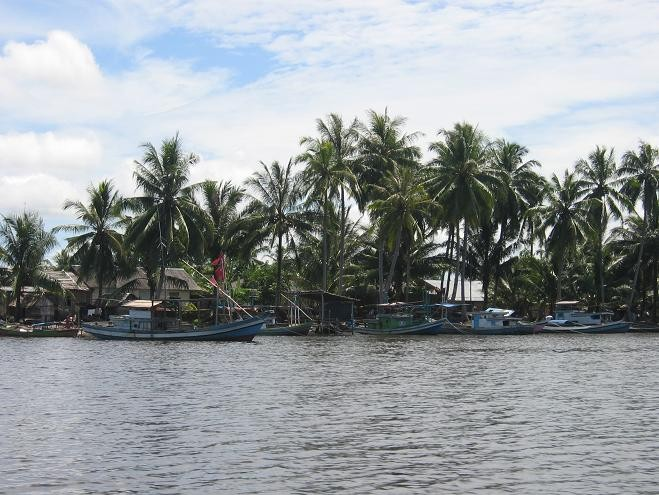
\includegraphics[width=5cm]{articles/Borneo/1210331303F4qq.jpg}
%La cote.
\smallbreak

\smallbreak
\hspace*{-0.65cm}
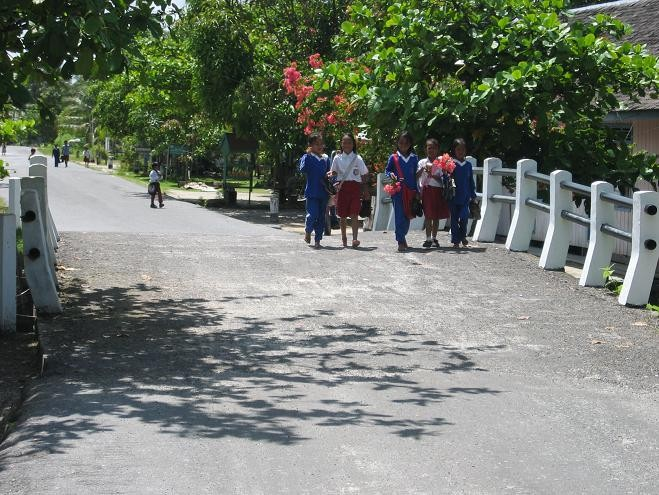
\includegraphics[width=5cm]{articles/Borneo/1210331297ISJ9.jpg}
%Rue centrale du village.
\smallbreak

Dès le lendemain nous nous sommes inscrits auprès d'un guide, pour pouvoir entrer dans la réserve et ainsi voir les Orang Outans. Ce qui paraissait au début être une belle arnaque s'est en fait avéré être une super journée, en pleine forêt tropicale.

\smallbreak
\hspace*{-0.65cm}
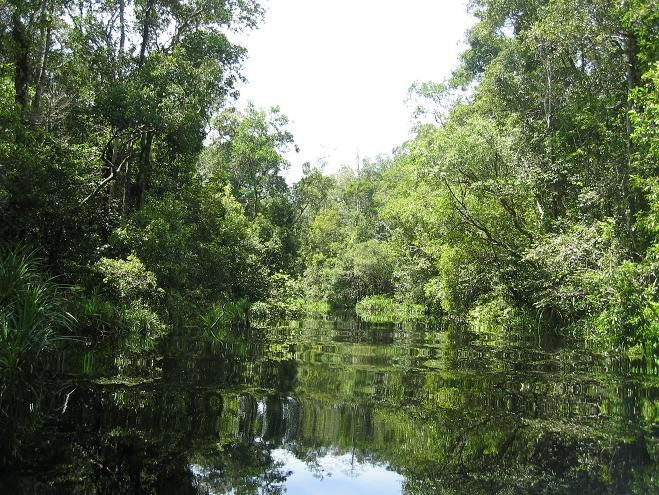
\includegraphics[width=5cm]{articles/Borneo/1210332087kPql.jpg}
%La mangrove.
\smallbreak

Nous avons assisté au repas de singes, en effet pendant la saison des fruits ils arrivent à se nourrir par eux même, mais en ce moment, la chose est plus difficile, les soigneurs apportent donc des bananes et les mettent sur des estrades, ce qui nous a permi, nous étions une poignée de personnes, de les regarder. En fait le plus impressionnant dans cette journée n'a pas été de les voir manger, mais plutôt de tomber au hasard d'un chemin sur l'un d'eux, de se faire un peu courser, puis de s'arrêter le regarder. Nous avons aussi vu des mamans garder leurs petits, c'était trop mignon.

\smallbreak
\hspace*{-0.65cm}
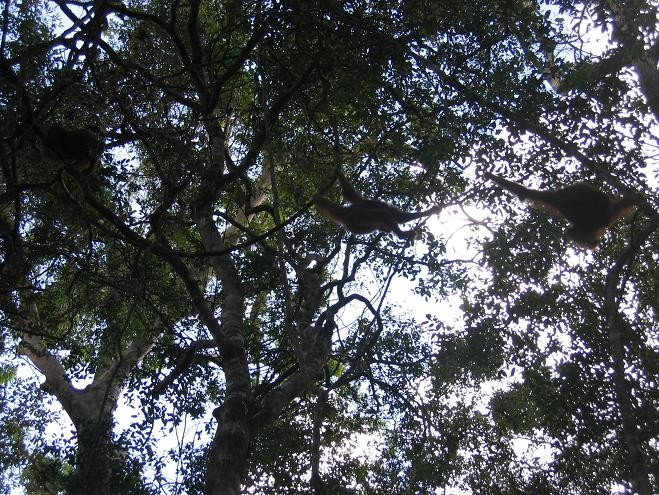
\includegraphics[width=5cm]{articles/Borneo/1210332096AngR.jpg}
%L'air de jeu des grands lascars.
\smallbreak

\smallbreak
\hspace*{-0.65cm}
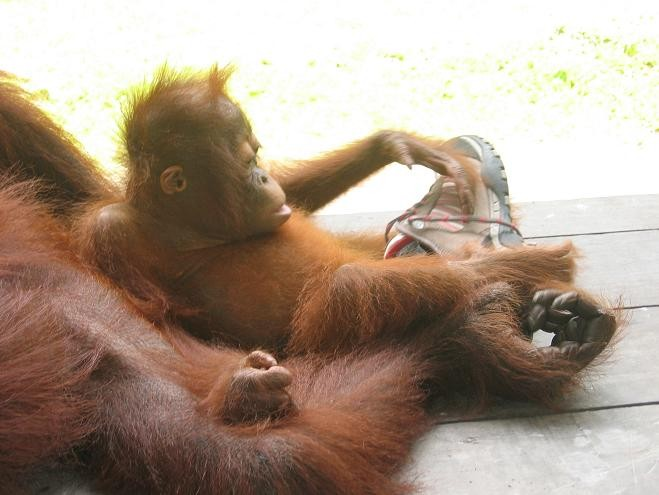
\includegraphics[width=5cm]{articles/Borneo/1210332100Imld.jpg}
%La nouvelle génération.
\smallbreak

%<div><object width="640" height="505"><param name="movie" value="http://www.dailymotion.com/swf/x5cnjc&v3=1&related=1"></param><param name="allowFullScreen" value="true"></param><param name="allowScriptAccess" value="always"></param><embed src="http://www.dailymotion.com/swf/x5cnjc&v3=1&related=1" type="application/x-shockwave-flash" width="640" height="505" allowFullScreen="true" allowScriptAccess="always"></embed></object></div>

\end{multicols}

\bigskip
\textbf{\textsc{Commentaires}}

\medskip
Nicoz a écrit le 19 juin 2008 :
\begin{displayquote}
Nan mais je rêve je suis le premier à poster sur cet article.
Bon je savais que t'avais bronzé et tout que t'avais pas forcément le temps de te raser sur le bateau mais là tout de même t'aurais pu me dire que tu t'étais teint en rousse :p
J'déconne mais ils sont trop mignons.
Bonne continuation
Continue à nous régaler des tes images.
\end{displayquote}

\vfill


%\pagebreak\section{Fiche de Singapour}

\begin{multicols}{2}

\smallbreak
\hspace*{-0.65cm}
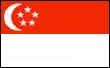
\includegraphics[width=5cm]{articles/Fiche-de-singapour/1210328633arj0.jpg}
%Drapeau de Singapour.
\smallbreak


\textbf{\textsc{Situation}}

\textbf{Présentation générale}

A l'extrême sud est de la péninsule malaise, la République de Singapour occupe une position stratégique à l'entrée du détroit de Malacca, qui longe la Malaisie au nord et Sumatra au sud. Sa superficie de 682,7 km2 se répartit entre une île principale d'environ 42 km (est-ouest) sur 23 km (nord-sud) et une soixantaine d'îlots. Séparée de la Malaisie par le détroit de Johore, d'à peine un kilomètre de large, elle est reliée au continent par une digue routière et ferroviaire, le "Causeway", et un pont à Tuas. Au sud, le détroit de Singapour la sépare de l'archipel indonésien de Riau. Le point culminant de l'île, le Timah Peak, est à 165 mètres au dessus du niveau de la mer.

\textbf{Liaisons avec la France}

11.000 km séparent Singapour de la France. Air France, Singapore Airlines et Quantas assurent des liaisons aériennes directes quotidiennes. Il existe par ailleurs de nombreux vols avec escales via Kuala Lumpur, Bangkok ou plusieurs capitales ou villes européennes (Londres, Amsterdam, Copenhague, Francfort...). Un vol direct dure environ 12h30.

\textbf{\textsc{Population}}

Principalement concentrée dans le sud de l'île, la population de 4 millions d'habitants compte 2,5 millions de Chinois, 382.000 Malais, 258.000 Indiens. Entre 1990 et 2000, la population non-résidente (étrangers vivant à Singapour depuis au moins un an) a presque doublé, passant de 10 à 19\% tandis que la part des résidents permanents s'élève à 7,2\%. En juin 2001, la population active comptait 2,12 millions de personnes.

|                                       |     SINGAPOUR   |    FRANCE    |
| ------------------------------------- |: -------------: | -----------: |
|Population                             |       4 millions| 59,2 millions|
|Densité                                |     6.055 hab.km2|   108 hab.km2|
|Accroissement naturel de la population |              1,7|           0,4|
|Indice de fécondité                    |              1,4|           1,8|
|Espérance de vie                       |           78 ans|      78,5 ans|
|Urbanisation                           |            100 \%|        75,6 \%|

\textbf{\textsc{Climat}}

Le climat est de type équatorial, chaud et humide toute l'année, avec une saison de fortes pluies de novembre à février. Les violents orages se montrent fréquents. La moyenne annuelle des températures s'établit de 24 à 34 degrés. Il n'y a pratiquement pas de variations saisonnières ni d'écart thermique entre le jour et la nuit. La pluviométrie annuelle moyenne est de 2500 mm. L'hygrométrie moyenne est de 84\%, avec un maximum de 96\% et un minimum de 64\%.

\textbf{\textsc{Villes principales}}

\textbf{Singapour}
Dans une mosaïque cosmopolite de quartiers (Chinatown, Kampong Glam, Little India, Orchard Road...), le centre ville, qui concentre les édifices publics et les hautes tours des affaires, se situe au sud de l'île. Entièrement reconstruit suivant un plan très aéré, il est doté de nombreux espaces verts. Des villes nouvelles entièrement constituées de blocs construits par le "Housing Development Board" se sont créées dans les banlieues : Ang Mo Kio, Bedok, Tampines, Clementi, Jurong. L'aéroport international de Changi, l'un des plus performants au monde, se trouve à l'est, sur l'île principale.

\end{multicols}

\vfill

%\pagebreak\section{Singapour, ville? pays?}

Date: 09/05/2008

\begin{multicols}{2}

Une fois n'est pas coutume, c'est deux articles que je vous écris aujourd'hui, je vous propose donc de retourner voir dans la rubrique Indonésie, l'article sur Bornéo.

Nous voici rendus à Singapour.

La première vue de cette ville, c'est le détroit de Malacca que nous passons en bateau, ce détroit est très impressionnant de par le nombre de cargos et portes conteners qui y sont arrétés, sans doute en attente de disponibilité d'un quai sur le port, pour pouvoir décharger. En effet Singapour est le plus gros port de commerce du monde, je croyais qu'il s'agissait de Rotterdam mais on m'a affirmé ici que c'etait Singapour, et à voir le traffic qu'il s'y passe, je veux bien le croire.

%<div><object width="640" height="505"><param name="movie" value="http://www.dailymotion.com/swf/x5d3be&v3=1&related=1"></param><param name="allowFullScreen" value="true"></param><param name="allowScriptAccess" value="always"></param><embed src="http://www.dailymotion.com/swf/x5d3be&v3=1&related=1" type="application/x-shockwave-flash" width="640" height="505" allowFullScreen="true" allowScriptAccess="always"></embed></object></div>

Voici une toute petite partie du port, nous l'avons longé durant 3 heure, c'est dire si il est long !!!

\hspace*{-0.65cm}
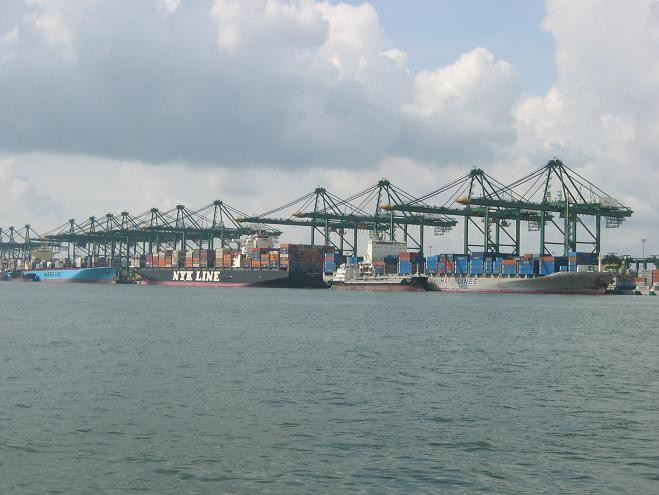
\includegraphics[width=4.8cm]{articles/Singapour-ville-pays/1210333644359c.jpg}
Port de Singapour


Que vous dire sur Singapour ???

Pour être clair, nous avons étés déçus par cette ville, trop clean, enclave de business au milieu de l'Asie. Je pourrais vous décrire avec de plus amples détails cette ville mais je vais préférer une image : Prenez la complexité d'une ville comme Paris, ajoutez y la propreté de Geneve (les amendes hors de prix pour le simple fait de jeter un papier faisant partie de la propreté) et rajoutez à cela un boom economique, des constructions nouvelles, comme dans un pays de pétrole, Dubaï, aux Emirats Arabes. Vous obtenez Singapour. Certe tout le monde parle anglais, on paie en dollars, tout est propre... mais pour moi il manque quelque chose !!!

Le tout vous donne une impression d'étouffer, cette ville est sympa à visiter mais pour rien au monde je ne viendrai y habiter.

Enclave parmis cela : Chinatown, le quartier chinois, où je retrouve le bordel que j'aime, ça grouille de partout, ça négocie, ca arnaque, il y a des boutiques de partout, sur on ne sait combien d'étages... Et nos cher geek trouveraient leur bonheur à Sim Lim Square, gros building de 7 étages entièrement remplis de boutiques d'informatiques, nous en avons profité pour faire réparer l'ordinateur portable qui nous avait laché juste après Bornéo. Et comme il etait vieux, Patrick se disant qu'il allait bientôt re-lâcher, il en a acheté un nouveau, résultat nous avons deux ordinateurs portables à bord... Et moi qui voulais faire un break !?!??!!?

Je vous laisse sur une photo de la marina où nous sommes restés durant notre séjour à Singapour

\hspace*{-0.65cm}
\includegraphics[width=4.8cm]{articles/Singapour-ville-pays/1210345462qOEk.jpg}
Piscine de la marina

A savoir : Le propriétaire d'un bateau ici est considéré comme étant obligatoirement riche, il n'existe donc pas de marina bon marché, le luxe est obligatoire (non je n'éxagere pas). Cela dit pour un "western" cela reste à la portée des bourses les plus légères, mais se voir proposer tout ce luxe est déconcertant à la fin, ça contraste avec nos journées en mer à prendre des douches à l'eau de mer, et uniquement se rincer à l'eau douce.

\end{multicols}

%\pagebreak\section{Fiche de la Malaisie}

Date: 17/05/2008

\begin{multicols}{2}

\textbf{\textsc{Drapeau}}

\hspace*{-0.65cm}
\includegraphics[width=4.8cm]{articles/Fiche-de-la-malaisie/1210328778gbyq.jpg}
Drapeau de la Malaisie.


\textbf{\textsc{Situation}}
\textbf{Présentation générale}

La Malaisie couvre une superficie de 330.000 hab.\kilo\meter\squared et comprend deux ensembles géographiquement distincts séparés par 800 \kilo\meter de mer :  Une partie péninsulaire de 131.000 hab.\kilo\meter\squared (750 \kilo\meter du nord au sud avec une largeur maximale de 350 \kilo\meter), montagneuse mais d'altitude peu élevée, partageant 506 \kilo\meter de frontière avec la Thaïlande au nord et bordée par Singapour au sud.
Une partie insulaire, formée de deux Etats au nord de l'île de Bornéo (Sabah et Sarawak), enclavant le Sultanat de Brunei et limitée par une frontière de 1.782 \kilo\meter avec l'Indonésie. Largement ouverte sur la mer, la Malaisie compte 4.675 \kilo\meter de côtes. La partie péninsulaire est baignée à l'ouest par le détroit de Malacca qui la sépare de l'île indonésienne de Sumatra ; à l'est se trouve la mer de Chine méridionale. Le Gunong Tahan (2187 m) est le point culminant dans la péninsule ; au Sabah, le mont Kinabalu (4101 m) représente le premier sommet de l'Asie du Sud-Est. Les deux ensembles qui composent la Malaisie ont en commun un climat équatorial, constamment chaud et humide, et un couvert forestier dense.

Les 11 Etats de la Malaisie péninsulaire sont :  ouverts sur la côte occidentale : Perlis, Kedah, Perak (frontaliers avec la Thaïlande), Penang, Selangor, Negeri Sembilan, Melaka Ouverts sur la côte orientale : Kelantan (frontalier avec la Thaïlande également), Terengannu, Pahang au sud : Johor.

\textbf{\textsc{Population}}

Des 24,5 millions d'habitants peuplant la Malaisie, environ 85\% sont concentrés dans la partie péninsulaire où ils sont inégalement répartis (de 22 hab.\kilo\meter\squared dans Pahang, l'Etat présentant la plus grande superficie, jusqu'à 926 hab.\kilo\meter\squared dans Penang, au nord ouest). Selangor (sur le détroit de Malacca) est l'Etat le plus peuplé avec 4 millions d'habitants. Un tiers de la population totale est âgé de moins de 15 ans. La population active représente près de 10 millions de personnes. Le recensement 2000 dénombrait 65\% de Bumiputras - "fils du sol" - 26\% de Chinois et 7,7\% d'Indiens. Un petit nombre de populations aborigènes subsiste en Malaisie (Orang Asli et tribus du Sarawak et du Sabah).

|                                       |     MALAISIE    |    FRANCE    |
| ------------------------------------- |: -------------: | -----------: |
|Population                             |    24,5 millions| 59,2 millions|
|Densité                                |     70,7 hab.\kilo\meter\squared|   108 hab.\kilo\meter\squared|
|Accroissement naturel de la population |               2 |          0,4 |
|Indice de fécondité                    |               3 |          1,8 |
|Espérance de vie                       |           72 ans|      78,5 ans|
|Urbanisation                           |             62 \%|         75,6\%|

\textbf{\textsc{Climat}}

Le climat est de type tropical humide avec des températures quasiment uniformes tout au long de l'année (minimum : 25 degrés, maximum : 37 degrés). Les précipitations les plus importantes sont reçues entre septembre et février (moyenne annuelle : 2700 mm). Cependant, un mois "sec" comporte encore près de 100 mm de pluie. L'hygrométrie est en permanence à plus de 80 \%.

\textbf{\textsc{Villes principales}}
\textbf{Kuala Lumpur}

Avec quelque 2 millions d'habitants - agglomération comprise - Kuala Lumpur constitue le centre économique et politique du pays. Dotée du statut de territoire fédéral depuis 1974 et placée sous le contrôle du gouvernement central, elle est enclavée dans l'Etat de Selangor (côte occidentale de la péninsule). Créée vers 1860, Kuala Lumpur est une ville cosmopolite et animée, caractérisée par une grande variété de styles architecturaux : maisons traditionnelles, architecture coloniale, bâtiments ultra-modernes dont les deux tours Petronas, les plus hautes du monde (450 m). L'aéroport international Klia se trouve à 75 \kilo\meter du centre-ville (soit 28 mn par train rapide). Depuis février 2002, la capitale est la ville nouvelle de Putrajaya, centre administratif du gouvernement fédéral, à 25 \kilo\meter au sud de Kuala Lumpur (www.pjholds.com.my).

\textbf{Autres villes}
Sur la péninsule : Georgetown, capitale de l'Etat du Penang. Ipoh, capitale de l'Etat de Perak. Johor Bahru, ville la plus méridionale et capitale de l'Etat du Johor.

\end{multicols}

%\pagebreak\section{Kuala Lumpur}

17 mai 2008

\begin{multicols}{2}

On entamme la Malaisie...

Eh oui, nous voici donc en Malaisie, toujours dans le détroit de Malacca séparant l'Indonesie et la Malaisie. Nous avons decide de faire une escale avant Langkawi, notre dernier arrêt avant d'entrer en Thaïlande. Ce sera Port Dickson, proche de Kuala Lumpur (KL pour les intimes). Nous arrivons à Port Dickson et la surprise on nous annonce qu'il y a un gros festival qui va se dérouler pendant les trois jour où nous sommes là, le freedom festival. C'est une sorte d'eurockéennes mais avec que de la musique techno-boum-boum, ils en raffolent ici...

Oui, mais bon, nous c'est pas notre truc... On préfère aller visiter Kuala Lumpur, on se renseigne sur comment y aller : ce sera 1/4h de bus, changement, 1h de bus, puis 1h de train. On nous a dit de descendre à KLCC, c'est là qu'il y a des trucs à voir. En fait il s'agit d'espèces de galeries Lafayettes de luxe : Gucci, Armani, Chanel... Ce qui nous fait croire que KLCC veux dire Kuala Lumpur Chopping Center, si vous avez une autre proposition je suis preneur. Nous pas contrariants, on y va, on sort de la station, on lève les yeux et regardez ce que l'on voit :

%\hspace*{-0.65cm}
%\includegraphics[width=4.8cm]{articles/Kuala-lumpur/1210432312E0e6.jpg}
%Tours Petronas.

Vous reconnaissez ? c'est les tours jumelles très connues de Kuala Lumpur, elles répondent au petit nom de tours Petronas et sont les tours jumelles encore debout les plus hautes du monde, il paraîtrait qu'il y a une banque au sommet, et c'est ici qu'a été tourné la fin du film Haute Voltige avec Sean Connery.

On continue et qu'est-ce que je vois... un bob AE qui se promène... il paraît qu'il fait le tour du monde (pour ceux qui ne voient pas de quoi je parle, rendez vous à la fin de l'article).

%\hspace*{-0.65cm}
%\includegraphics[width=4.8cm]{articles/Kuala-lumpur/1210432316GlgU.jpg}
%Tours Petronas again.

Allez c'est décidé on marche un peu, on mange un bout, et au detour d'une rue...

%\hspace*{-0.65cm}
%\includegraphics[width=4.8cm]{articles/Kuala-lumpur/1211015560vRGE.jpg}
%Un peu de chauvinisme.

Y a pas à dire la tour Eiffel et Zidane, restent les deux élément connus partout dans le monde quand on parle de la France.

Bon c'est pas tout ça mais nous on leve encore les yeux au ciel et on voit encore des choses sympa, en particulier cette tour, la 4ème la plus haute du monde avec ses 421 mètres de haut.

%\hspace*{-0.65cm}
%\includegraphics[width=4.8cm]{articles/Kuala-lumpur/1211014906Nl6S.jpg}
%Tour qui s'appelle je sais plus comment.

Qu'est-ce qu'on doit avoir une belle vue de la haut... allez hop on y va...

%\hspace*{-0.65cm}
%\includegraphics[width=4.8cm]{articles/Kuala-lumpur/1211014913RrBL.jpg}
%Vue d'en haut de la tour (qui tourne...)

Moi qui adore voir les choses de loin, et du plus haut possible, j'étais servi. Kuala Lumpur sur 360 degrés.

Retour sur le plancher des singes, en dehors de ses grattes-ciel KL redeviens une ville ressemblant à beaucoup de capitales, si ce n'est que tout est nickel, presque comme à Singapour. Mais allez savoir pourquoi, a KL je me sentais bien, loin de l'impression que j'ai eu à Singapour.

Je vous laisse sur deux photos de la ville en elle même.

%\hspace*{-0.65cm}
%\includegraphics[width=4.8cm]{articles/Kuala-lumpur/1211016874hbIL.jpg}
%Ben... la rue quoi.

%\hspace*{-0.65cm}
%\includegraphics[width=4.8cm]{articles/Kuala-lumpur/1211017229ryCi.jpg}
%Monorail aérien.

\end{multicols}

 * Le bob autour du monde, kesako ? A l'UTBM il y a eu un message de passé incitant toutes les personnes voyageant autour du monde à emporter un bob AE (Association des Etudiants) et à le prendre en photos devant les grands endroits connus où l'on pourrait aller.

\bigskip
\textbf{\textsc{Commentaires}}

\medskip
Titou a écrit le 18 mai 2008 :
\begin{displayquote}
Je n'ai qu'une chose à dire : petit enfoiré ! C'est franchement magnifique ! Tu m'étonnes que tu te sentes bien là-bas. Merci de prendre quelques instants pour nous en faire profiter, ça fait du bien de voyager un peu par ces temps de gros taff. Continue de t'éclater et à plus ! Biz mon pote !
Ps : ton truc anti-spam ça claque! Après faut gérer les additions\dots t'as pa pensé à ça toi! heureusement on a pu m'aider pour répondre :p
\end{displayquote}

\medskip
Peggy a écrit le 18 mai 2008 :
\begin{displayquote}
Pareil que "titou" je suis en panique là, je me concentre fort pour ne pas oublier la réponse au fameux calcul anti-spam (aujourd'hui: 8+2) et du coup je conclue très vite en te faisant des biz.
SEE YOU.
\end{displayquote}

\medskip
Etienne a écrit le 19 mai 2008 :
\begin{displayquote}
Ah oui évidement les pré-requis sont peut être un peu élevés pour certains, mais en s'y mettant à plusieurs pour repondre je pense que c'est faisable.
Merci à vous deux qui prenez toujours le temps de laisser un message, les autres vous savez quoi faire, et à tous les "occasionnels", qui ont peut être étés refroidis par le spam, ça y est c'est fini, vous pouvez revenir !
Je vous promet encore des superbes photos pour venir compléter l'article sur Langkawi, cette île est vraiment top!!!
\end{displayquote}

\medskip
Gege (rien) a écrit le 19 mai 2008 :
\begin{displayquote}
Alors pour ceux à qui le petit calcul fait tellement peur : Menu démarrer --> Programmes --> accesoires --> calculatrice :)
Des tours aussi hautes, ça me fout tout le temps le vertige : j'imagine même pas les jours de grands vents, comment la tour doit bouger, ça doit foutre la g****
\end{displayquote}

\medskip
Zan a écrit le 19 mai 2008 :
\begin{displayquote}
Et dire que j'étais dans cette ville il y a un peu plus d'un an et que j'ai rien vu de tout ça!!! C'est super beau, grand\dots
Enfin bon c'est ça d'avoir juste 2 heures d'escale à Kuala Lumpur en faisant Paris-Sydney, je suis pas sorti de l'aéroport\dots Mais bon ce sera pour une prochaine fois :D
Enjoy, c'est vraiment magnifique tout ça!
\end{displayquote}

\vfill


%\pagebreak\section{Langkawi}

17 mai 2008

\begin{multicols}{2}

Aujourd'hui au programme, les iles Langkawi où je suis actuellement. Il s'agit des dernières îles malaisiennes avant la Thaïlande, c'est donc ici que nous ferons tamponner nos passeports avant de remonter. Nous sommes arrivés au Sud et avons dormi une nuit au mouillage dans une petite crique bien sympa.

%<div><object width="640" height="505"><param name="movie" value="http://www.dailymotion.com/swf/x5lrr0&related=1"></param><param name="allowFullScreen" value="true"></param><param name="allowScriptAccess" value="always"></param><embed src="http://www.dailymotion.com/swf/x5lrr0&related=1" type="application/x-shockwave-flash" width="640" height="505" allowFullScreen="true" allowScriptAccess="always"></embed></object></div>

Puis c'est reparti on remonte un peu au nord pour aller dans une marina, on compte rester quelques jours ici. Et là je dois le dire, car c'est assez rare pour être souligné, même Patrick a été impressionné par la beauté de l'endroit (oui, on a pas tous la chance d'avoir vécu en Calédonie). L'entrée de la marina est tout simplement superbe.

\smallbreak
\hspace*{-0.65cm}
\includegraphics[width=5cm]{articles/langkawi/1211018197eneE.jpg}
%Plage de Langkawi.
\smallbreak

\smallbreak
\hspace*{-0.65cm}
\includegraphics[width=5cm]{articles/langkawi/1211018204F7Ee.jpg}
%Entrée de la marina.
\smallbreak

\smallbreak
\hspace*{-0.65cm}
\includegraphics[width=5cm]{articles/langkawi/1211018457DniB.jpg}
%Ben... sortie de la marina... le même endroit, quoi.
\smallbreak

Et c'est parti pour visiter, pas loin de la marina il y a des chutes d'eau. On voulait au départ aller prendre un téléphérique qui monte au sommet de la colline pour voir toute l'île mais il était en réparation, ce n'est que partie remise.

\smallbreak
\hspace*{-0.65cm}
\includegraphics[width=5cm]{articles/langkawi/1211018190Pmip.jpg}
%Cascade.
\smallbreak

Je complèterai cet article dans les jours qui viennent avec des photos du tour de l'île, je vais louer un scooter car il parait que ça vaut vraiment le coup...

Je vous laisse sur une petite note poissonistique.

%<div><object width="640" height="505"><param name="movie" value="http://www.dailymotion.com/swf/x5gab6&v3=1&related=1"></param><param name="allowFullScreen" value="true"></param><param name="allowScriptAccess" value="always"></param><embed src="http://www.dailymotion.com/swf/x5gab6&v3=1&related=1" type="application/x-shockwave-flash" width="640" height="505" allowFullScreen="true" allowScriptAccess="always"></embed></object></div>

Voici comme promis quelques photos en plus.

\smallbreak
\hspace*{-0.65cm}
\includegraphics[width=5cm]{articles/langkawi/1212397933wQ6v.jpg}
%La marina vue d'en haut.
\smallbreak

\smallbreak
\hspace*{-0.65cm}
\includegraphics[width=5cm]{articles/langkawi/1212398042f2k1.jpg}
%Une passerelle touristique.
\smallbreak

\smallbreak
\hspace*{-0.65cm}
\includegraphics[width=5cm]{articles/langkawi/1212397931akoQ.jpg}
%Petit ponton dans la mangrove.
\smallbreak

\end{multicols}

\bigskip
\textbf{\textsc{Commentaires}}

\medskip
Titou a écrit le 18 mai 2008 :
\begin{displayquote}
Je me répète\dots mais on ne gère pas tous l'addition :p ! Attand on est qu'à l'UTBM, ça fait partie du programme de dernière année  et y en a qui n'y son pas encore\dots
Allez enjoy and take care. Biz ma poule.
\end{displayquote}

\medskip
Peggy a écrit le 19 mai 2008 :
\begin{displayquote}
ETIENNE LE JUSTICIER (des petits poissons)!!
Je me demande ce qu'il se passerait si tu sautais à l'eau, ils essayeraient de te grignoter les fesses peut être?
Bon, je sors!
Avant\dots petite réflexion 7+1=? (heureusement que les calculs restent simples!)
\end{displayquote}

\medskip
Etienne a écrit le 20 mai 2008 :
\begin{displayquote}
Y en a un qui m'a gniaqué le doigt, j'avais posé un bout de pain dessus et approché de l'eau car ce sont des poissons cracheurs, ils visent le bout de pain et le font tomber pour le récupérer. Seulement celui-ci m'a mordu le doigt, le suivant a mis un coup de boule dans le pain pour le faire tomber.
\end{displayquote}

\medskip
Pierre a écrit le 26 mai 2008 :
\begin{displayquote}
Hey!
C'est vrai que la plage est blasante\dots j'ai connu mieux!!!
Non sérieusement ça fait halluciner!
Continue de vendre du rêve!
Gad m'a rappelé : je lui ai proposé de te laisser un message sur ton blog\dots
Biz à toi.
\end{displayquote}

\medskip
Titou a écrit le 26 mai 2008 :
\begin{displayquote}
ON VEUT LA SUITE ! ON VEUT LA SUITE !
A BIENTOT TI DUD !
\end{displayquote}

\medskip
Tite soeur a écrit le 28 mai 2008 :
\begin{displayquote}
Pour moi, 4+8=12\dots ça reste simple\dots
On est le 28, et pas de nouvelle depuis le 20\dots va falloir penser à ceux qui restent en France et qui commencent à s'inquéter\dots
Donne nous des news\dots
A bientôt ti frère
Bisou.
\end{displayquote}

\vfill


%\pagebreak\section{Fiche de la Thailande}

Date: 30/05/2008

\begin{multicols}{2}

\textbf{\textsc{Drapeau}}

\hspace*{-0.65cm}
\includegraphics[width=4.8cm]{articles/Fiche-de-la-thailande/drapeau_thailande.png}
Drapeau de la Thaïlande

\textbf{\textsc{Situation}}

D’une superficie de \SI{513.115}{km^2}, sensiblement égale a la France, la Thailande s’etend du 5e au 21e parallele, soit sur pres de 1770 km de long ; sa plus grande largeur d’est en ouest est de 805 km mais se reduit a 50 km a la hauteur de l’isthme de Kra.
Elle est limitée a l’est et au nord-est par le Laos, au sud-est par le Cambodge, au sud par la Malaisie, au nord-ouest et a l’ouest par la Birmanie. On distingue cinq regions principales :

La région centrale, vaste plaine alluviale du Menam Chao Phraya, le plus grand fleuve thailandais. Cette plaine bien arrosee et iriguee, constituee de riches sediments, est a la fois le grenier a riz du pays, son centre historique avec Bangkok, industriel, urbain et financier. Elle est bordee a l’est par le Cambodge et donne au sud sur le golfe de Thailande. C’est la region la plus peuplee.

La région montagneuse du nord et de l’ouest, qui longe la frontiere birmane et culmine au mont Doi Inthanon (2 595 m), peu peuplee, recouverte de forets.

La région est ou s’etend un plateau greseux aride, le plateau du Korat, bordant la vallee du Mekong, qui separe la Thailande du Laos. La region nord-est est une region pauvre et rurale, avec de petites exploitations qui ne supportent plus qu’une recolte annuelle. 15\% des terres sont cultivees et l’elevage du gros betail est dominant. Les importants travaux d’irrigation n’ont pas eu les retombees esperees.

La région sud-est comprend les massifs de Dongrek et de Khao Khieu qui delimitent la frontiere avec le Cambodge ;

Le sud, situe sur la presqu’ile de Malacca est borde a l’ouest par la Birmanie et la mer d’Andaman. Cette region, soumise a la mousson, est tres arrosee. A l’est on trouve le golfe de Thailande et au sud la Malaisie. Cette zone bien arrosee produit le riz, l’hevea, pratique la peche et dispose aussi de ressources minieres (zinc).

\textbf{\textsc{Population}}

80\% des Thaïlandais sont des Thaïs, un ensemble de peuples originaires de la Chine occidentale. Les Chinois constituent la minorité la plus importante, environ 10\% de la population. Parmi les autres minorités figurent les musulmans (1,5 million) d’origine malaise qui vivent dans le Sud, les "tribus" montagnardes du nord (Karens, Hmongs, Akhas, Lahus), les réfugiés Viêtnamiens et Cambodgiens (Khmers) et une importante population de travailleurs Birmans "clandestins" (environ 800.000).

|                                       |     THAILANDE   |    FRANCE    |
| ------------------------------------- |: -------------: | -----------: |
|Population                             |    61,2 millions| 59,2 millions|
|Densite                                |      \SI{118}{hab.km^2}|   \SI{108}{hab.km^2}|
|Accroissement naturel de la population |              1,1|           0,4|
|Indice de fecondite                    |             1,87|           1,8|
|Esperance de vie                       |           69 ans|      78,5 ans|
|Urbanisation                           |           43,3 \%|        75,6 \%|

\textbf{\textsc{Climat}}

Le climat de la Thaïlande est tropical et humide. On distingue trois saisons :
- une saison sèche très chaude (mars - juin)
- une saison des pluies (juillet - octobre)
- une saison plus fraîche (novembre - février).
On note de grandes variations climatiques en fonction des regions. Dans l’ensemble l’amplitude thermique est faible en Thaïlande. Les températures moyennes mensuelles à Bangkok varient entre 31 et 35 degrés C sur l’année. Le degré hygrométrique varie de 45 a 85\%.

\textbf{\textsc{Villes principales}}

\textbf{Bangkok}
Capitale et plus grande ville du royaume (8 millions d’habitants, 12 millions avec la banlieue), située au centre du pays, sur les rives du Menam Chao Phraya, près du golfe de Siam. Bangkok est un des grands carrefours commerciaux du Sud-Est asiatique et un important port de transit qui assure la majorité des échanges exterieurs du pays. La ville, située dans une région productrice de riz, est aussi le premier centre industriel du pays (agro-alimentaire, textile, ciment, pétrole raffine et constructions mécaniques). La ville est le siège du Comité économique et social des Nations unies pour l’Asie et le Pacifique ainsi que de l’Organisation du traité de l’Asie du Sud-Est (OTASE). Centre de la culture et de l’enseignement thaï, Bangkok compte plusieurs universités et collèges techniques. On peut y admirer quelques 400 temples somptueusement décorés (les wats) dont le Wat Phra Kaeo (Temple du boudha d’émeraude) situé à l’intérieur des murs du Grand Palais. Elle est parcourue de très nombreux canaux et les marchés flottants, où les embarcations servent de lieux de vente, sont encore très actifs. La ville est tres polluée et est connue pour ses embouteillages légendaires.

\textbf{Chiang Mai}
Située à environ 720 km au nord de Bangkok et à 130 km de la frontière avec la Birmanie, sur la rivière Ping, la ville est le grand centre économique du nord de la Thailande (500.000 habitants) ainsi qu’un terminus ferroviaire. La ville ancienne conserve les vestiges de temples datant du 13ème et 15ème siècles, dont celui du Wat Phra Dhat Doi Suthep censé abriter les reliques de Bouddha. Outre le tourisme, la ville vit du commerce du teck, de ses productions agricoles et de ses objets artisanaux (laques, poteries, produits de luxe).

\textbf{Nakhon Ratchasima}
Située au Nord-Est du pays, à 256 km de Bangkok, sur le fleuve Moun, dans la partie méridionale du plateau de Khorat. La ville compte 204.000 habitants. C’est un centre industriel (matériel ferroviaire, agroalimentaire, tissages) et commercial mais également un centre universitaire et l’un des hauts lieux du bouddhisme.

\end{multicols}

%\pagebreaklayout: landscape
title: Phuket
date: 2008/05/30 14:58:25
tags:
---

Salut tout le monde...

Comment ça je me fais attendre, je vois vraiment pas de quoi vous voulez parler... Mais l'avantage quand les articles sont éspacés dans le temps c'est qu'à priori il va y en avoir plus à lire !! Premièrement j'ai ajouté une video (au debut) et 3 photos (à la fin) sur l'article de Langkawi.

Nous voici donc repartis en mer de Langkawi direction Phucket en quelques jours, avec haltes sur différentes îles se trouvant sur notre chemin. But avoué : faire de la plongée car la mer devenait enfin claire. Depuis l'Indonésie impossible de plonger, à certains endroit on ne voyait à peine le bout de notre bras dans l'eau. Tous ça c'est bien joli, mais c'était compter sans les nuages et la pluie qui rendent la plongée tout de suite moins agréable. Enfin bon on va pas se pleindre quand meme.

Nous passons près de Koh Lanta, ça vous dit quelque chose ?

<div><object width="640" height="505"><param name="movie" value="http://www.dailymotion.com/swf/x5lrzm&related=1"></param><param name="allowFullScreen" value="true"></param><param name="allowScriptAccess" value="always"></param><embed src="http://www.dailymotion.com/swf/x5lrzm&related=1" type="application/x-shockwave-flash" width="640" height="505" allowFullScreen="true" allowScriptAccess="always"></embed></object></div>

Puis nous voici arrivés à Ko Phi Phi, île très touristique, bien que nous soyons en basse saison, le trop plein de monde est blasant. Voici quand meme une belle photo, c'est le plus beau coté de la plage principale, l'autres coté étant occupé par des hôtels, restos, boutiques à souvenir...



Charlotte, tu reconnais ?

Mais Ko Phi Phi c'est pas pour le tourisme que vous aviez peut être déjà ce nom dans la tête, c'est un des endroits qui a été le plus touché par le tsunami en 2004 et du coup maintenant on se retrouve avec pleins de panneaux de partout indiquant où aller en cas d'alerte.



Vous remarquerez au passage l'écriture thaï, non non ce n'est pas de la décoration pour faire joli, c'est bien du texte... En plus de ça pour une même orthographe, un mot peut avoir jusqu'à 5 significations differentes suivant sa prononciation. Aprenez le thaï, qu'il disait !!

Ca y est, on arrive a Phuket. Et la, question tourisme, on est en plein dedans : des plages, du béton et... de la prostitution. Phuket Town, la plus grosse ville de l'île échape un peu à ça, c'est sympa de s'y ballader, on retrouve le quartier chinois, le marché couvert...

<div><object width="640" height="505"><param name="movie" value="http://www.dailymotion.com/swf/x5lrj3&related=1"></param><param name="allowFullScreen" value="true"></param><param name="allowScriptAccess" value="always"></param><embed src="http://www.dailymotion.com/swf/x5lrj3&related=1" type="application/x-shockwave-flash" width="640" height="505" allowFullScreen="true" allowScriptAccess="always"></embed></object></div>

Sur le reste de l'île, des plages...



... et Boat Lagoon, la marina où nous nous sommes arrêtés pour sortir le bateau. En effet Patrick a besoin de faire un carrénage sur le bateau (remettre de la peinture spéciale anti coquillages appelée anti fulling sur la coque) et faire quelques réparations.





Bon... et j'avais pas dit qu'une fois arrivé a Phuket je reprenais mon sac, moi? C'est partiiiiiiii !!!

Jeudi matin, mon sac est fait, je quitte Patrick et son bateau perché à 4 mètres de haut direction Phuket Town. Il faut que j'achète le Lonely Planet car je n'ai pas de guide de la Thaïlande, et que je prenne le bus direction Hua Hin, entre Phuket et Bangkok. Première librairie : pas de guide. Deuxième : les Lonely Planet sont au rayon fiction, ca promet... et ils n'ont pas la Thaïlande, c'est vrai que c'est quand même beaucoup plus utile d'avoir le Brésil ou l'Australie à Phuket. Et puis ils sont aimables comme des portes de prisons, j'arrête, je vais prendre le bus.

Hua Hin please. Je paie, je monte dans le bus, il est 12h30, je n'ai aucune idée du temps de trajet. En premier on me dit 5h, puis 7, puis... j'arrive à 1h du matin apràs plus de 12 heures de trajet. Je marche un peu, refuse les désormais classiques taxi qui proposent des "cheap hôtel", et zou, je trouve une petite guest house pour dormir, la seule du coin à être ouverte 24h/24 à priori. Bon en même temps je stressais pas trop car Hua Hin est située le long de la mer, et si je ne trouvais rien je serais allé dormir sur la plage, il fait chaud ici y a pas de soucis.

Voila, je crois que je vous ai donné un peu de lecture, à bientôt.

%\pagebreak\section{Bangkok}

12 juin 2008

\begin{multicols}{2}

Alors alors... Je vous ai laissés à Hua Hin, petite ville en passe de devenir une grosse station balnéaire à 3 heures de bus de Bangkok. Je n'ai pas énormément de choses à vous dire à propos de cette ville, si ce n'est que le patron de la guest house "All Nations" est Anglais, et qu'il est fan de tennis. Nous avons regardé Roland Garros ensembles. Je suis resté 3 nuits a Hua Hin puis j'ai pris le bus pour Bangkok.

Pout tout vous dire j'ai hésité à appeler cet article "Marchés a Bangkok", ou "Marcher à Bangkok". C'est donc tout logiquement que j'ai choisi un troisième titre.

Bangkok... très grande ville, bien sympa à découvrir. On peut trouver tout ce que l'on veut il suffit de bien chercher. Cependant si vous voulez une montre Rolex ou une écharpe Gucci, le premier petit marchand ambulant fera l'affaire... Bien sûr n'allez pas lui demander un reçu ou un certificat de conformité.

J'ai été très bien accueilli par Cécile, une amie de mes parents qui est prof de maths à Bangkok, puis Célia, sa fille, nous a rejoint, elle rentrait d'un stage de 3 mois au Viêtnam. Autant vous dire qu'on a pas arrété de parler de voyages.

La visite de la ville a commencé en prenant un bateau sur un des klongs, les klongs sont des canaux, pas toujours accueillants par leur odeur, mais permettant de voir un coté non touristique. Une petite photo pour se mettre dans l'ambience, et la video après.

%\hspace*{-0.65cm}
%\includegraphics[width=4.8cm]{articles/Bangkok/1345.jpg}
%Bateau sur un Klong.

%<div><object width="640" height="505"><param name="movie" value="http://www.dailymotion.com/swf/x5n17d&related=1"></param><param name="allowFullScreen" value="true"></param><param name="allowScriptAccess" value="always"></param><embed src="http://www.dailymotion.com/swf/x5n17d&related=1" type="application/x-shockwave-flash" width="640" height="505" allowFullScreen="true" allowScriptAccess="always"></embed></object></div>

Puis je suis allé voir le Jim Thomson museum. Il s'agit d'un petit musée regroupant la collection d'art d'un certain Jim Thomson comme vous l'aurez compris. J'ai surtout apprécié ça pour l'architecture des petites maisons en bois, on ne s'attend pas à voir ça en plein centre de Bangkok.

%\hspace*{-0.65cm}
%\includegraphics[width=4.8cm]{articles/Bangkok/1338.jpg}
%Une Pagode du Thomson Museum.

Puis je me suis balladé dans la ville, je suis resté en tout un peu plus de 4 jours à Bangkok. Les Thaïlandais adorent leur roi, et ils le montrent. Le lundi est le jour du roi et il est impressionnant de voir le nombre de Thaïs qui s'habillent en jaune (sa couleur) ce jour là. Ils adorent aussi montrer leur drapeau accompagné du drapeau du roi (symbole royal sur fond jaune). Voici une photo d'un batiment.

%\hspace*{-0.65cm}
%\includegraphics[width=4.8cm]{articles/Bangkok/1395.jpg}
%Un bâtiment dans Bangkok, avec pleins de drapeaux.

Comme j'aime bien le bateau (vous le saviez?), je n'ai pas pu m'enpêcher de naviguer sur la Chao Praya, fleuve qui coule du côté Ouest de Bangkok, et c'est l'occasion de vous présenter des bonzes. Un bonze est un prêtre ou moine bouddhiste, très respecté de tous. J'ai fait attention à ne pas les faire tomber dans l'eau, ça aurait fait mauvais genre de couler un bonze dans la rivière (amis des mauvais jeux de mots, bonjour).

%\hspace*{-0.65cm}
%\includegraphics[width=4.8cm]{articles/Bangkok/1396.jpg}
%Les bonzes sur la Chao Praya.

Un truc que j'adore maintenant, c'est visiter les marchés. Ici on voit tout, du plus propre (quoique...) au plus sale, mais tout le monde achète et finalement tout se passe bien. En fait c'est nous qui avons un sens du propre trop développé je pense. Cela dit la majorité des stands sont de très bonne qualité, il faut juste fermer les yeux quand on passe devant certains stands de poisson ou de viande.

%\hspace*{-0.65cm}
%\includegraphics[width=4.8cm]{articles/Bangkok/1384.jpg}
%Un marché

%\hspace*{-0.65cm}
%\includegraphics[width=4.8cm]{articles/Bangkok/1387.jpg}
%Une autre photo du marché

%<div><object width="640" height="505"><param name="movie" value="http://www.dailymotion.com/swf/x5r4b7&related=1"></param><param name="allowFullScreen" value="true"></param><param name="allowScriptAccess" value="always"></param><embed src="http://www.dailymotion.com/swf/x5r4b7&related=1" type="application/x-shockwave-flash" width="640" height="505" allowFullScreen="true" allowScriptAccess="always"></embed></object></div>

Je ne vous dis pas au revoir ici, j'attaque directement l'article suivant sur Kanchanaburi.

\end{multicols}

\bigskip
\textbf{\textsc{Commentaires}}

\medskip
Titou a écrit le 15 juin 2008 :
\begin{displayquote}
Ehehe encore de jolies photos mon petit Dud !
En ce qui concerne le coulage des bonzes\dots je dirai que bizarrement le cerveau arrive a lire des mot qui ne sont pas forcément complets\dots mais je t'apprendrai ! il faut un R :) Content de te savoir en vie et en pleine forme. Profites a fond car ici c'est la misère\dots
Fais gaffe a toi et a plus.
Biz mon pote
\end{displayquote}

\vfill


%\pagebreak\section{Kanchanaburi}

Date: 12/06/2008

\begin{multicols}{2}

Avant de commencer la lecture, avez vous lu l'article sur Bangkok que je viens d'écrire? (oui je fais les articles deux par deux maintenant, allez savoir pourquoi).

Kanchanaburi vous connaissez ? Mais si, faites un effort...

Bon je vais poser la question autrement : Le pont de la rivière Kwai, vous connaissez? Allez pour ceux qui n'ont pas vu le film, bref rappel historique : Nous sommes en cinquante avant Jesus Christ, heu non, là je me trompe d'histoire... Le pont à été construit par les Japonais pendant la seconde guerre mondiale. Enfin quand je dit par les Japonais je devrais plutôt dire par leur prisonniers. 9.000 prisonniers sont morts durant sa construction, ce qui est particulièrement étonnant quand on voit la taille du pont. Le film, lui, a eu 6 oscars et reste le 13ème film le plus vu au monde.

Je suis allé à Kanchanaburi pour voir le pont du film, non pas pour dire "j'y étais", mais plus car dans le film le pont a l'air vraiment impressionnant, et puis tant qu'à être dans le coin.... Seulement c'est un faux!!! En vrai le pont ne fait pas plus d'une cinquantaine de mètres, il est en béton et en fer, non pas en bois. Assez parlé, je vous le montre.

\hspace*{-0.65cm}
\includegraphics[width=4.8cm]{articles/Kanchanaburi/1400.jpg}
Le pont de Kanchanaburi.

\hspace*{-0.65cm}
\includegraphics[width=4.8cm]{articles/Kanchanaburi/1401.jpg}
Le train qui passe sur le pont.

Petite déception pour Kanchanaburi, donc. d'autant plus que je ne suis pas le seul à me faire avoir, au final la ville est remplie de touristes, la rivière est remplie de speed boats qui font un max de bruit. Y'a même des boîtes de nuit flottantes... Y sont fous ces romains!!!

Va falloir faire autre chose de sympa dans le coin, car même en louant une motor bike je n'ai pas vraiment été séduit par les alentours. Je propose les chutes d'eau d'Erawan, à deux heures de bus de là, vous êtes d'accord?

Juste avant de partir j'ai rencontré deux francaises bien sympas (là je fais le faux jeton passqu'elle m'ont promis qu'elles passeraient voir ce blog, Anna et Geraldine, si vous me lisez...) qui arrivaient juste et qui ne savaient pas trop où aller en premier, nous sommes donc allés à Erawan ensembles.

Ces chutes sont sur 7 niveaux où il est possible de se baigner. Inutile d'en dire plus, je vous laisse regarder.

\hspace*{-0.65cm}
\includegraphics[width=4.8cm]{articles/Kanchanaburi/1440.jpg}
Les chutes d'Erawan.

\hspace*{-0.65cm}
\includegraphics[width=4.8cm]{articles/Kanchanaburi/1439.jpg}
L'est pas bizarre ce rocher ?

\hspace*{-0.65cm}
\includegraphics[width=4.8cm]{articles/Kanchanaburi/1437.jpg}
Un p'tit tobogan.

\hspace*{-0.65cm}
\includegraphics[width=4.8cm]{articles/Kanchanaburi/1438.jpg}
Et un bassin.

Bon, y a quand même un truc qu'il faut vous dire. Dans tous les bassins, il y a des poissons. Et alors? me direz vous. Un poisson, c'est sympa, mais quand ça a faim, ça l'est moins. Ajoutez à cela un appetit particulier pour les talons d'européens et vous en tirez une sensation assez spéciale qui a un arrière goût de n'y reviens pas. La seule solution était donc de bouger sans arrêt dans l'eau, et on a finit par trouver un petit bassin/jacousie ou y en avait pas.

\begin{dialogue}
  \speak{Moi} Bon c'est bien beau tout ca, mais le dernier bus est à quelle heure?
  \speak{Anna} A 16h
  \speak{Moi} Et il est ?
  \speak{Anna} 16h05...
\end{dialogue}

On essaie de voir avec un groupe de 4 personnes qui avaient loué un tuk tuk collectif (ca passe à 7 largement dedans). Pas moyens. Et là notre négociatrice en chef (Anna) demande a un Thaï qui a un pick-up si il va a Kanchanaburi, il y va, il peut nous emmener. Et c'est parti pour faire le retour dans son coffre, les cheveux au vent (et un peu à la pluie), sympa l'expérience.

Et après Kanchanaburi me direz vous, c'est vrai que ça fait un bout de temps que vous n'aviez pas nouvelles. J'ai pris le bus pour Ayutaya, au nord de Bangkok, mon but était d'aller à Chiang Mai sans repasser par Bangkok. Je me suis donc arrêté une journée dans la petite ville d'Ayutaya, et y ai loué un velo pour me ballader. J'ai ensuite pris un bus pour Chiang Mai de nuit (10h de route, on s'est fait offrir le cafe à 6h du mat' en arrivant). Et me voici donc a Chiang Mai pour une semaine environs, avant d'aller au Laos. Ma première expérience de la journée à Chiang Mai est une amande mise par un flic hilard alors que je voulais tourner à droite en motor bike là où c'était interdit. J'ai du le suivre au commissariat pour récupérer mon permis, et là, comme par hasard, l'interdiction de tourner à droite ne s'applique plus... Ca me rappelle Bali tout ça.

Voila, l'article est finit, vous pouvez éteindre votre ordinateur et reprendre une activité normale.

\end{multicols}

\bigskip
\textbf{\textsc{Commentaires}}

 \medskip
Peggy a écrit le 12 juin 2008 :
\begin{displayquote}
ah! de la lecture, des images, des vidéos!! tout ce que l'on aime...
quel grand périple, mais, tu rentres qd (si tu rentres un jour!!) :p
Bisous
Take care!
2+9=11
\end{displayquote}

 \medskip
Etienne a écrit le 13 juin 2008 :
\begin{displayquote}
Je rentre vers mi juillet, je ne sais pas encore precisement car je n'ai pas encore pris mon billet, le tout est que je trouve un appart a Paris avant le debut de mon stage, le 11 aout.
D'ici la, Laos... et retour a Bali.
\end{displayquote}

 \medskip
Jaco a écrit le 14 juin 2008 :
\begin{displayquote}
Eh ben mon ptit Dud, on se la coule douce pendant que d'autres travaillent !
En tout cas profite bien des merveilles de l'exostisme...
Jaco ;)
\end{displayquote}

 \medskip
Titou a écrit le 15 juin 2008 :
\begin{displayquote}
Bali quand tu nous tiens .... :p
Ralala tu n'es vraiment qu'un petit salopiaud ! Dire que y en a qui sont a l'agonie et sous des tonnes de taff.... pff t'es cruel !
Profites mon pti profites !
Merci encore pour ces images et commentaires et fais toi bien plaiz !
A plus ti dud et take care !
ps : Bali ... pourquoi bali ?? ... :p
\end{displayquote}

 \medskip
Nicoz a écrit le 19 juin 2008 :
\begin{displayquote}
Salut ptit Dud,
Alors tu vois que je te met des com aussi en plus de te parler sur MSN :p
Bon d'accord j'avoue jle fais pas à chaque fois mais bon.
Sinon bah profite bien du Laos j'attend les photos et profite bien de Bali et de l'exotisme local ;)
Bonne continuation de ton périple.
Moi jserais toi jsais pas si je reviendrai pour retourver la grisaille parisienne :p
\end{displayquote}

 \medskip
Organisatrice de stages a écrit le 20 juin 2008 :
\begin{displayquote}
bonjour,
chose promise, chose due... même si cela a tardé un peu, je viens de jeter un oeil à votre blog. (en rappel d'un précédent mail : je ne sais pas si cela fera causer vos copains ? vous me direz).
La lecture de votre texte sur Kanchanaburi me donne bien envie de lire plus. Dès que je me serai débarrassée de tous les étudiants récalcitrants (je maintiens ;-)), je ferai une petite pause lecture...
j'en profite aussi pour autre chose : j'ai reçu de Thailande une carte ANONYME ce matin. Comme, contrairement à la plupart des courriers anonymes, elle était plutôt sympa :) Alors merci beaucoup pour le geste.
Bonne continuation dans vos tribulations,
\end{displayquote}

 \medskip
Etienne a écrit le 22 juin 2008 :
\begin{displayquote}
Oups... j'ai pas signe
\end{displayquote}



%\pagebreak\section{Chiang Mai}

26 juin 2008

\begin{multicols}{2}

Amis du voyage, Bonjour !!!

Je voyage maintenant et encore pour quelques jours avec Arnaud, un français bien sympa rencontré à Chiang Maï.

Aujourd'hui nous allons parler de Chiang Mai, ville du nord de la Thaïlande dans laquelle je suis resté 5 jours. En fait, plutôt que de vous parler de Chiang Mai, je vous propose de parler des environs de Chiang Mai, car comme à mon habitude maintenant je ne suis pas trop resté dans les murs de la ville mais j'ai préféré louer une motor bike pour aller é la campagne, voir des gens que le tourisme ne touche pas... et que l'anglais ne touche pas non plus, d'où pas mal de difficultés, et de gêne.

Nous sommes allés nous ballader avec Arnaud, jeune Français comme moi qui fait un voyage en Asie de deux mois.

Direction le nord, où nous suivons une route de montagne sur une trentaine de kilomètres. Puis un autre jour, nous descendons au Sud, environs 80km pour aller dans un parc national. Nous nous arrêtons le midi dans un petit warung (genre snack pas cher) pour manger un riz frit ou autre fried noodles et nous tombons sur deux mecs, bien saouls, la bouteille de whiskey à moitié vide sur la table. Ils nous invitent à venir nous joindre à leur table. Vu qu'on est pas du genre à dire non, on y va. Et là on s'aperçoit vite que c'était un traquenard, en fait on est la curiosité du moment et d'autres mecs arrivent, on boit tous, on se fait offrir une soupe aux crevettes, on boit, on prend des photos, on boit... Bon c'est pas tous ça mais le temps est très gris, saisons des pluies oblige, on a décidé d'aller voir le parc, et de faire les 80km pour rentrer après, va falloir y aller molo sur la picole !!!

\smallbreak
\hspace*{-0.65cm}
\includegraphics[width=5cm]{articles/Chiang-mai/1214286196a5oS.jpg}
%Bah c'est du propre, tiens !
\smallbreak

\smallbreak
\hspace*{-0.65cm}
\includegraphics[width=5cm]{articles/Chiang-mai/1214286184dsFU.jpg}
%Soupe de piment.
\smallbreak

Mon passage a Chiang Mai n'aurait pas été le même sans la Julie's Guest House, c'est pourquoi je me dois d'en dire quelques mots. Le concept : les chambre les moins chères que j'ai vues en Thailande, les boissons à volonté (il suffit de marquer ses consommations sur un carnet dédié et on paie a la fin), plusieurs espace de détente où il est très facile de rester une journée entière à discuter avec d'autres voyageurs, jouer au billard... ou regarder l'euro 2008 à 2h du matin.

\smallbreak
\hspace*{-0.65cm}
\includegraphics[width=5cm]{articles/Chiang-mai/1214471834JD3r.jpg}
%La Julie's guest house, au top !
\smallbreak

Pour terminer, et parce que j'ai envie de vous poser une question qui n'a rien à voir, voici une devinette : Devinez le nom de ce très bon fruit.

\smallbreak
\hspace*{-0.65cm}
\includegraphics[width=5cm]{articles/Chiang-mai/1214471825EGhM.jpg}
%Mais quelle est ce fruit ?
\smallbreak

\end{multicols}

\bigskip
\textbf{\textsc{Commentaires}}

\medskip
Titou a écrit le 26 juin 2008 :
\begin{displayquote}
eheh ! Encore de jolies photos que voila ! Comme tu le vois je n'ai pas pu attendre ce soir ni demain pour faire ma lecture !
Ralala ça donne envie, tu me raconteras tout ça en détails devant une bonne bière à ton retour !
A plus ti dud !
ps : pour le fruit j'ai pas trouvé alors c'est pour ça que j'ai rien dit :p
\end{displayquote}

\medskip
Chachou a écrit le 27 juin 2008 :
\begin{displayquote}
Coucou,
Toujours des photos qui font envie (quoi que la soupe de crevettes, pas plus envie que ça...).
On gagne quoi si on répond bien à la devinette?
Fruit du dragon ou pitaya rose à chair blanche
Bonne continuation
Bisous ;-)
\end{displayquote}

\medskip
Etienne a écrit le 27 juin 2008 :
\begin{displayquote}
Ok Chachou, bien joue c'est un fruit du dragon. Je t'aurais bien dit que tu en gagnes un mais il risquerais de ne plus etre bon apres 10 jours a Bali. Et comme ton mec ne veux pas que je te fasse de bisous, ben du coup je vais essayer de trouver une autre idee.
\end{displayquote}



%\pagebreaklayout: blog
title: Pai
date: 2008/06/26 12:17:32
tags:
---

Pai... petite ville encaissée dans les montagnes, au Nord Ouest de Chiang Mai, dans le triangle d'or de la drogue aux frontières du Myanmar, du Laos et de la Thaïlande. Pai a donc été mon étape suivant Chiang Mai. Je devais y retrouver là deux Québécois pour aller au Laos ensuite avec eux. Ce que j'avais pas vu c'est qu'en fait, ces deux jeunes frère et soeure sont du genre je dit un truc et je fais l'inverse. Du coup je les ai vite oubliés.

Durant les trois heures de bus pour Pai, j'ai rencontré Ammar, photographe et videaste Syrien. Nous avons passé une bonne partie des quatre jours ensemble.



Nous avons là encore fait des tours en motor bike, pour se ballader, prendre des photos...

<div><object width="640" height="505"><param name="movie" value="http://www.dailymotion.com/swf/x5x4t5&related=1"></param><param name="allowFullScreen" value="true"></param><param name="allowScriptAccess" value="always"></param><embed src="http://www.dailymotion.com/swf/x5x4t5&related=1" type="application/x-shockwave-flash" width="640" height="505" allowFullScreen="true" allowScriptAccess="always"></embed></object></div>




Et regardez ce que l'on voit au detours d'un chemin : une guest house qui vous propose de dormir dans un arbre :



Mais bon... la mienne c'est celle la :



J'en profite pour vous présenter Abby et Sue, deux Anglaise avec lesquelles on a passé un peu de temps aussi.

Revenez ici de temps en temps, des photos vont s'ajouter.

%\pagebreak\section{Fiche du Laos}

Date: 26/06/2008

\begin{multicols}{2}

\textbf{\textsc{Drapeau}}

\hspace*{-0.65cm}
\includegraphics[width=4.8cm]{articles/Fiche-du-laos/1214470058Q382.jpg}
Drapeau du Laos.


\textbf{\textsc{Situation}}
\textbf{Presentation générale}

Avec une superficie de 236.800 km2, le Laos est enclavé au coeur de la péninsule Indochinoise. Il est bordé à l’Est et au Nord par le Viêtnam et la Chine, et limite à l’Ouest et au Sud par la Birmanie, la Thaïlande et le Cambodge.

Le Mekong traverse le Laos sur 1.898 km et dessine le principal axe du pays.

Le point culminant du Laos, le Phou Bia avec 2820 m, se trouve au sud du plateau de Xieng-Khouang. Une quinzaine d’autres sommets dépassent 2000 m.

\textbf{\textsc{Population}}

Au Laos, soixante-huit groupes ethniques sont officiellement recensés. Parmi les plus importants, il faut citer les Lao Lum, ou Lao des plaines, représentant 45 a 50\% de la population, les Lao Theung, ou Lao des vallées, comptant pour 30\% et les Lao Sung ou Lao des montagnes, dont les 15\% se répartissent en Hmongs, Meos ou Yaos.

|                                       |       LAOS      |    FRANCE    |
| ------------------------------------- |: -------------: | -----------: |
|Population                             |     5,2 millions|  	59 millions|
|Densite                                |     22,8 hab.km2|   108 hab.km2|
|Accroissement naturel de la population |              2,8|          0,46|
|Esperance de vie                       |           59 ans|     78,86 ans|
|Urbanisation                           |            17 \%|      75,6 ans|

\textbf{\textsc{Climat}}

Le Laos est un pays au climat tropical humide, marqué par deux saisons :

- La saison sèche de septembre à avril, agréable en décembre janvier, très chaude en mars et avril : la température est comprise entre 14 degres et 25 degrés.
- La saison des pluies d’avril a septembre, tres humide et tres chaude, avec des orages frequents : la temperature est comprise entre 30degres et 44 degrés.

\textbf{\textsc{Villes principales}}
\textbf{Vientiane}

Vientiane est la capitale politique et économique du Laos. Située sur la rive gauche du Mékong, elle compte environ 370.000 habitants. Elle devint pour la première fois capitale sous le regne du Roi Pothisarath (1520-1548). Elle fut rasée en 1826 par les Thaïs et retrouva son rang de capitale sous l’impulsion des Français au debut du XXème siècle.

\textbf{Luang-Prabang}

Luang-Prabang, avec 110.000 habitants, est l’ancienne capitale royale. Située au confluent de la Nam Khan et du Mékong, sur un site privilégié de la préhistoire, elle est la ville la plus riche du pays en pagodes.

\textbf{Savannakhet}

Forte de 147.000 habitants, Savannakhet est un port fluvial important, au carrefour d’un des postes frontières ouverts pour le commerce avec la Thaïlande et de la route menant au Viêtnam (Da-Nang).

\textbf{Pakse}

Avec 72.000 habitants, au carrefour des routes vers la Thaïlande et le Cambodge, cette ville est l’ancien fief de la famille de Champassak qui régnait sur le Sud.

\end{multicols}

\vfill

%\pagebreak\section{Mekong}

Date: 26/06/2008

\begin{multicols}{2}

Mékong, Mékong... ça me dit quelque chose...

Mais oui c'est bien ça, le fleuve qui part de Chine, fait la frontière entre le la Thaïlande et le Laos puis va au Cambodge. Je suis parti de Pai en bus direction Chiang Khong, ville Thai faisant face a Huay Xay, ville Laotienne. C'est donc là que j'ai passé les deux postes d'émigration et d'immigration, puis je me suis enbarqué sur un bateau pour descendre sur le Mékong vers Luang Prabang, en deux jours.

Pour cet article, exceptionnelement je ne vous propose que des photos, en effet le recit de ces deux jours tient en deux mot : chill out.

\hspace*{-0.65cm}
\includegraphics[width=4.8cm]{articles/Mekong/1214473370zy1a.jpg}
Le bateau vu en longueur.

\hspace*{-0.65cm}
\includegraphics[width=4.8cm]{articles/Mekong/12144733896AMi.jpg}
Des enfants sur la berge.

\hspace*{-0.65cm}
\includegraphics[width=4.8cm]{articles/Mekong/1214473395mtro.jpg}
Encore une escale.

\hspace*{-0.65cm}
\includegraphics[width=4.8cm]{articles/Mekong/1214473400ezNu.jpg}
Un village sur la côte.

\hspace*{-0.65cm}
\includegraphics[width=4.8cm]{articles/Mekong/1214473407uNUm.jpg}
Escale du soir.

\end{multicols}

\bigskip
\textbf{\textsc{Commentaires}}

\medskip
Titou a écrit le 13 juil. 2008 :
\begin{displayquote}
Eh ti dud !
Bon je voulais juste mettre un petit post sur ton blog pour ne pas laisser ce blanc tout pas beau en bas de ton message! Profites bien de tes derniers jours et je te dis à très bientôt !
Biz mon pote
\end{displayquote}

\medskip
Helene et Dova a écrit le 14 juil. 2008 :
\begin{displayquote}
Coucou Etienne!
Alors content de retrouver ta petite ile indonesienne :-)?
Nous venons de naviguer sur ton blog, et nous n'avons pas trouve de photos recentes. Aurais tu d'autres choses plus interessantes a faire?
Nous attendons toujours avec impatience les photos de Vang Vieng.
Aussi, nous n'avons pas ton e-mail.
Quand repars tu de Bali? Nous Arrivons le 23.
A bientot la bas, par mail ou mieux encore a Paris.
Cheers Helene \& Dova
\end{displayquote}

\medskip
Helene \& Dovaline a écrit le 11 sept. 2008 :
\begin{displayquote}
Hola guapo!!!
Alors tu te fais a la vie parisienne? La ligne 2, c'est quoi ça??? Nous avons décidé d'effacer tous les mauvais souvenirs. Nous ne voulons meme pas penser au retour a Paris et d'ailleurs on se demande si on va vraiment rentrer.
Nous sommes actuellement au Chili, a Valparaiso. Demain nous partons pour le Nord. Nous remontons lentement ce pays avant de rejoindre la Bolivie et le Perou. Ici il fait froid, on a du se refaire au plus vite une garde-robe. Lávantage c que nous avons a notre grande surprise pu skier a seulement 42 kms de Santiago... Grandiose et grand ciel bleu. Faudra aller voir les photos sur le blog.
Envoie nous ton mail perso sur notre adresse mail stp et aussi nous sommes impatientes d'enfin voir les photos de Vang Vieng.
A bientôt mais pas trop tôt car on encore soif de decouverte.
Muchos besos
Helene \& Dova
\end{displayquote}



%\chapter{Pérou et Bolivie}
%\section{Fiche du Pérou}

Date: 10/10/2009

\begin{multicols}{2}

\textbf{\textsc{Drapeau}}

\hspace*{-0.65cm}
\includegraphics[width=4.8cm]{articles/Fiche-du-perou/1255177646Fug0.jpg}
Drapeau du Pérou

\textbf{\textsc{Le Pérou en chiffres}}

** Capitale : ** Lima
** Superficie ** : \SI{1285216}{km^2}
** Habitants ** : 29.925.628 (en 2005)
** Habitants de la capitale : ** 7.500.000
** Densité de la population : ** \SI{17,2}{hab.km^2}
** Religion : ** En majorité catholique ; minorité protestante et animiste

\textbf{\textsc{Géographie et territoire}}

Situé dans la partie centre occidentale de l'Amérique du Sud, le Pérou s'étend sur une superficie de \SI{1285216}{km^2}, y compris les \SI{4996.28}{km^2} de la partie péruvienne du lac Titicaca.

Traversé sur toute sa longueur par la section centrale de la Cordillère des Andes, le Pérou est constitué de trois zones géographiques bien distinctes : la côte, surtout désertique, qui s'étend sur une longueur de 2.414 km, occupe 7\% de la superficie totale et il s'élève de manière progressive de l'Océan Pacifique vers la Cordillère. La Sierra, constituée par la chaîne montagneuse andine, qui occupe 33\% de la superficie, et il a son sommet le plus élevé dans le Huascaràn (6.768 m) ; la forêt, constituée par l'aire amazonienne à climat tropical, qui occupe 60\% du territoire dans la zone orientale du Pays, et elle est traversée, dans la partie septentrionale, par les affluents du Rio des Amazones (parmi lesquels il y a le fleuve le plus long du Pérou, le Marañàn, qui s'étend sur 2406 Km).

La Cordillère des Andes est formée par une section Orientale, constituée pour la plupart de rochers paléozoïques, et qui rejoint les sommets les plus élevés au sud dans la zone du fleuve Urubamba (Auzangate, 6384 m) ; par une section Centrale, à caractère moins unitaire et avec des sommets moins élevées ; par une section Occidentale, constituée surtout de granite. L'aire volcanique la plus étendue se trouve dans la partie méridionale du Pays, et rejoint son altitude la plus élevée avec le Misti à 5822 m.

\textbf{\textsc{Population}}

La population du Pérou est particulièrement composite, surtout à cause des trois siècles de domination espagnole. Le groupe ethnique le plus représentatif est constitué de quechua (45\%), puis de métis (37\%), de créoles (12\%), de blancs (15\%), de aymarà (4\%), et d'autres minorités parmi lesquelles, non recensée, celle des indios de la jungle, estimés à 30.000 en 1981.

A peu près la moitié de la population vit sur les hauts plateaux en pratiquant une agriculture de pure subsistance, tandis que seulement 6\% habite dans l'immense bassin amazonien. Rappelez-vous que le terme "indios" est considéré péjoratif, il vaut beaucoup mieux utiliser le mot "indigenas".

\textbf{\textsc{Climat}}

Au Pérou, les saisons sont renversées par rapport à notre hémisphère : l'été, chaud et très pluvieux, trouve son sommet entre novembre et février ; l'hiver, avec un climat tendanciellement tempéré et extrêmement sec, couvre la période de mai à septembre.

La situation climatique ressent de toute manière la différente situation géomorphologique du pays : la meilleure période pour visiter le Pays, au moins pour se rendre sur le haut plateau et dans l'Amazonie, et celle qui va de juin à aout, grâce à l'absence presque totale de pluies, en se rappelant toutefois que sur les Andes l'amplitude thermique entre le jour et la nuit est très élevée (l'on va aussi sous zéro), et qu'un vêtement conforme est indispensable.

Ceux qui se rendent sur la cote, au contraire, trouvera un climat variable de 15 à 25 degrés, mais aussi une petite brume humide uniforme (garua) qui empêche de voir le soleil jusqu'à 800 mètres d'altitude.

\textbf{\textsc{Heure}}

Le Pérou a 6 heures en moins par rapport à la France (lorsqu'il est 12 heures en France, au Pérou il est 6 heures), et cette différence d'horaire passe à 7 heures pendant notre période d'horaire d'été.

\textbf{\textsc{Langues}}

Les langues officielles sont l'espagnol et le quechua, même si l'aymarà résulte très répandu, en particulier dans la zone du lac Titicaca.

D'autres dialectes sont enfin parlés dans les 50 communautés, d'indiens amazoniens de la forêt.

Se souvenir que l'anglais est vraiment peu répandu et même l'espagnol peut ne pas être suffisant avec la population amérindienne de la sierra.

\textbf{\textsc{Religion}}

La religion dominante au Pérou, grâce à la longue domination espagnole, est sans doute celle catholique (92,4\% de la population). Une minorité résulte protestante (5,5\%), tandis que parmi les Amérindiens les cultes animistes sont très répandus. Les populations autochtones tendent à mélanger la religion catholique aux anciennes religions traditionnelles avec des offrandes à Pachamama ou aux dieux de la montagne (apus).

\end{multicols}

\bigskip
\textbf{\textsc{Commentaires}}

\medskip
Titou et Chachou a écrit le 11 oct. 2009 :
\begin{displayquote}
Aller hop, on inaugure le blog même si c'est avant que tu partes !
On te souhaite un très bon voyage, profites en bien et surtout fais bien gaffe à toi !
On te suivra au jour le jour (enfin si y a des nouvelles quoi :p) et on attendra de tes nouvelles avec impatience !
Allez bon vol et take care.
Grosse léchouille de nous deux :-D
\end{displayquote}

\medskip
Salah Eddine a écrit le 18 oct. 2009 :
\begin{displayquote}
hello mec,
Comment ça va la bas. toujours pas de nouvelles photos depuis les préparatifs. il faut les mettre pour qu'on suive.
Allez, je te laisse profiter, mais tiens nous au jus.
A+
Salah.
\end{displayquote}


%\pagebreak\section{Derniers préparatifs}

Date: 11/10/2009

\begin{multicols}{2}

Bonjour à tous !!

C'est reparti pour un tour, je m'envole pour l'Amérique latine cette fois pour aller découvrir la culture Inca et les beaux paysages de la Cordillère des Andes. A l'heure où je vous écrit, il est 21h, dimanche soir et je décolle demain matin à 10 heure pour une boucle de 5 semaines essentiellement au Pérou et en Bolivie, mais rien n'est réellement fixé et il se peut très bien que j'aille faire un petit tour au Chili, en Argentine, au Paraguay ou au Brésil. En fait le choix se fera réellement sur place, en fonction des rencontres, et peut-être aussi des mouvements sociaux (l'Est de la Bolivie est parfois à éviter), je me renseignerai sur place.

Alors sur une carte, ça donne quoi ?

\hspace*{-0.65cm}
\includegraphics[width=4.8cm]{articles/Derniers-preparatifs/1255286224vDMd.jpg}
Carte du Pérou


J'atterris à Lima mardi matin, à l'aube (ma journée de lundi aura duré 31h), de là je pars vers le sud par la côte, et je pense m'arrêter à Pisco, juste au dessus de Ica. Et la s'arrêtent les plans, vous lirez la suite ici car je ne la connais pas encore...

Allez, si, j'ai deux destinations à aller voir : Le Machu Pichu, situé près de Cuzco et à une altitude telle qu'il faut du temps pour s'y habituer, puis le Salar Uyuni (désert de sel) situé au Sud de la Bolivie, au Sud Ouest de Potosi.

Sur ce je vous dit à bientôt ici même, j'essaierai de mettre un article toutes les semaines environs (sous réserve de cyber cafés disponible).

Etienne

\end{multicols}

\bigskip
\textbf{\textsc{Commentaires}}

\medskip
Sam a écrit le 11 oct. 2009 :
\begin{displayquote}
Bon voyage! J'ai hate de lire la suite de tes aventures, petit chanceux !
\end{displayquote}

\medskip
Pegg a écrit le 11 oct. 2009 :
\begin{displayquote}
et seras tu accompagné ? Have a good trip :)
\end{displayquote}

\medskip
Ahlem a écrit le 11 oct. 2009 :
\begin{displayquote}
Ca y est c'est le départ?!
Génial, je suis sûre que ça va être super bien cette "escapade latine".
Bon voyage et amuses toi bien!!!
Ahlem
\end{displayquote}

\medskip
Abanon a écrit le 11 oct. 2009 :
\begin{displayquote}
Bon voyage ! profites en bien !
\end{displayquote}

\medskip
Jaco a écrit le 12 oct. 2009 :
\begin{displayquote}
Enfoiré :)
\end{displayquote}

\medskip
Nicoz a écrit le 12 oct. 2009 :
\begin{displayquote}
Bon voyage et profite bien !
\end{displayquote}

\medskip
Cécile a écrit le 12 oct. 2009 :
\begin{displayquote}
Hé hé, bon voyage! :D
\end{displayquote}

\medskip
Etienne a écrit le 13 oct. 2009 :
\begin{displayquote}
Merci pour vos messages ¡¡¡

Ca y est j'ai atterri a Lima, apres une escale a Miami ou j'ai eu le temps d'aller me ballader sur south beach et de tester les transports en commun du coin\dots eh bien y a un truc de clair c'est qu'en France on a pas a rougir de la qualite de nos bus! J'ai eu droit a un petit florilege de tous nos prejuges sur le americains, mais surtout, tous ceux avec qui j'ai discute etaient super sympa..
C'est decide au retour je prevois mon maillot de bain dans le petit sac cette fois pour aller me baigner entre les deux avions.
Peggy, je suis parti seul.. on prend le meme et on recommence :)
A bientót
\end{displayquote}

\medskip
Philippe a écrit le 14 oct. 2009 :
\begin{displayquote}
Rhâââ\dots Tu n'as pas prévu de maillot de bain pour les sources thermales au pied du Machu Pichu ;-)

Have a nice trip!
\end{displayquote}

\medskip
Yohann a écrit le 15 oct. 2009 :
\begin{displayquote}
Et mec, trop cool l'amerique latine. Amuse toi bien. Et si tu passes en patagonie, prend un max de photo, je prévoie d'y aller en janvier, j'pourrais avoir un aperçu :-)
Léchouilles
PS: trop facile l'anti-spam\dots
\end{displayquote}

\medskip
Helene (ta colloc) ;-) a écrit le 15 oct. 2009 :
\begin{displayquote}
Bon, je vois que tu as atterri, c déjà un bon point.
Par contre tu avais juré de nous donner des nouvelles, heureusement qu'on prend les devants.
Ici ca va, entretiens, entretiens, entretiens\dots ca devient presque une routine et Dova comme d'hab, boulot, boulot, boulot\dots
Allez enjoy, et ne nous oublie pas trop vite!
On pense à toi.
Bisous
Les croqueuses du monde (enfin c'est un peu révolu ca!)
\end{displayquote}

\medskip
Dova (ton autre coloc') a écrit le 16 oct. 2009 :
\begin{displayquote}
Holà, holà!

Révolu?! On n'a pas dit notre dernier mot!
En attendant de croquer de nouveaux horizons, on compte sur toi pour nous faire vibrer durant ces 5 semaines\dots
Hasta pronto y cuidado guapo,
Muchos besos de las mujeres de mundo :))
\end{displayquote}

\medskip
Zé a écrit le 16 oct. 2009 :
\begin{displayquote}
Como estàs Etienne? disfrutando me imagino\dots
Profite bien señor! J'attends la suite avec impatience!
Hasta luego!
\end{displayquote}

\medskip
Dodo a écrit le 18 oct. 2009 :
\begin{displayquote}
Ouaich mon Dud, fait toi bien plaisir, c'est tout ce que je te demande !! En Inde tout s'est super bien passé c'était de la boulette à 7 ! On a souvent pensé à toi\dots Et tes biddies attendent sagement
La bise
\end{displayquote}

\medskip
Helene (ta colloc) ;-) a écrit le 20 oct. 2009 :
\begin{displayquote}
Salut!
Bon alors, c qd que tu le remets à jour ton blog????
Bz
\end{displayquote}

\vfill


%\pagebreak\section{Côte du sud}

20 oct. 2009

\begin{multicols}{2}

Bonjour,

Alors alors, par où commencer... Ah oui, par le premier jour..

Nous sommes lundi 12, je suis à l'heure a l'aéroport, mon avion est à l'heure lui aussi, je demande confirmation pour savoir si l'arrière de l'appareil dessert bien Miami lui aussi comme il est indiqué à l'avant :), et c'est parti pour un survol de l'atlantique, 10h de vol, 12h de transit forcé sur le sol Américain car l'aeéoport n'a pas de zone internationale, je vais voir la plage, me balade dans Miami, sympa cette escale..

%\hspace*{-0.65cm}
%\includegraphics[width=4.8cm]{articles/Cote-du-sud/1255996649K0tQ.jpg}
%Miami beach.

Puis c'est reparti pour 6 heures de vol direction Lima, capitale du Perou, la je decouvre une ville immense (8 million d'habitants) aux différents quartiers très différents. Du quartier très pauvre où me laisse le collectivo (minivan transformé en minibus très cheap).

%\hspace*{-0.65cm}
%\includegraphics[width=4.8cm]{articles/Cote-du-sud/1255996655Vfsf.jpg}
%Quartier pauvre de Lima.

Au quartier déjà un peu plus riche autour de la Plaza de Armas, ici une photo d'une bâtiment du gouvernement qui borde la Plaza de Armas. Je découvrirais plus tard que chaque ville comporte une place de ce nom, et il s'agit en général d'une place richement décorée, contrastant avec les alentours.

%\hspace*{-0.65cm}
%\includegraphics[width=4.8cm]{articles/Cote-du-sud/1255996660JAoN.jpg}
%Plaza de Armas.

Reprenons le fil des choses, je suis arrivé à 4h30 du matin et j'ai attendu un peu le jour avant de sortir de l'aéroport, j'ai eu le temps de me renseigner comment éviter les taxis hors de prix puis me voila avec mon sac dans un collectivo bondé direction le centre de Lima, il me dépose un peu  à l'extérieur où vous avez pu voir le Lima mal famé, puis je marche vers la place des armes où je vais me renseigner à l'office du tourisme pour des bus en direction du Sud, vers Pisco où il y a de belles choses à voir lorsqu'on a le pied marin. Des bus partent toutes les 8 minutes, c'est presque trop facile... Je passe le reste de la matinée à me ballader dans Miraflorès, quartier chic de Lima (tout est relatif) au bord de la falaise qui donne sur l'océan, puis je prend mon bus pour Pisco. Je visiterai plus en détail Lima à mon retour avant de revenir sur le vieux continent.

%\hspace*{-0.65cm}
%\includegraphics[width=4.8cm]{articles/Cote-du-sud/1255996643RUpx.jpg}
%Peru moderno.


Pisco, ville touchée par un séisme deux ans plus tôt, tout est en reconstruction, on sent vraiment la pauvreté ici. Le Lonely Planet me dit de me méfier, l'hôtel me dit de sortir sans sac, de cacher mon appareil photo et de laisser mon passeport dans le coffre fort de la chambre (pourtant j'avais pris une chambre sans option, le coffre est de serie, ça laisse présager..). Quoi de mieux pour faire flipper le voyageur en visite ? Je ne me suis jamais senti en insécurite à Pisco, les gens sont sympa, l'extrême pauvreté alliée à l'aridité du sol donne à la ville un caractère étrange.

%\hspace*{-0.65cm}
%\includegraphics[width=4.8cm]{articles/Cote-du-sud/12559974777RC0.jpg}
%Pisco.


Allez, une petite photo d'un étalage, parce que vous le valez bien.

%\hspace*{-0.65cm}
%\includegraphics[width=4.8cm]{articles/Cote-du-sud/1255997490cIfD.jpg}
%Marché de Pisco.


Heureusement pour les Piscoñeros, une belle richesse est aux portes de la ville, il s'agit des iles Balestas, véritable condensé de faune (pas très) sauvage, ainsi qu'un mystère archéologique. Un chandelier a été tracé il y a des centaines d'années dans le sable sur le flanc d'une montagne, et l'énigme irrésolue est de savoir comment il se fait que le dessin ne s'efface pas. Nous voyons ce chandelier d'un bateau en allant voir les îles Balestas. Les deux théories étant que le dessin est sur une face sous le vent, donc protégée, et que la sédimentation aurait durci le sol. Quoiqu'il en soit il est interdit de débarquer pour aller vérifier.

%\hspace*{-0.65cm}
%\includegraphics[width=4.8cm]{articles/Cote-du-sud/1255997496rIn7.jpg}
%Chandelier de Paracas.


Et nous voici sur les îles, ici vit un grand nombre de pélicans pingouins, lions des mers et plein d'autres oiseaux..

%\hspace*{-0.65cm}
%\includegraphics[width=4.8cm]{articles/Cote-du-sud/1255997482Hoy0.jpg}
%Pélicans aux Balestas.


Regardez moi cette star...

%\hspace*{-0.65cm}
%\includegraphics[width=4.8cm]{articles/Cote-du-sud/1255997520UtdU.jpg}
%Who is the boss ?


Me voila reparti sur la route direction Ica, et surtout Huacachina, petit Oasis touristique au milieu des dunes pour faire du sandboard, activité vivement conseillée par mes très chères colocs qui l'ont pratiquée un an plus tôt et en ont encore le sourire aujourd'hui quand elles en parlent (Hélène et Dova, merci pour le conseil, je me suis régalé !!). Le concept ? Une oasis entourée de dunes qui sert de camp de base pour partir deux heures en areñeros, sorte 4*4 au design lunaire avec lequel on va à fond dans les dunes, dévalant les pentes et dérapant de partout, puis séance de sandboard, snowboard des sables. Et bien vous savez quoi ? on se dit que c'est facile quand on sait faire du snow, et en fait ça l'est pas tant que ça, mais bon j'ai quand même réussi à faire mes virages et quelques belles descentes.

Voici votre envoye special au debut du tour..

%\hspace*{-0.65cm}
%\includegraphics[width=4.8cm]{articles/Cote-du-sud/1255997503PLr1.jpg}
%Areneros.


Pour le concept du sandboard, c'est par ici..

%\hspace*{-0.65cm}
%\includegraphics[width=4.8cm]{articles/Cote-du-sud/1255997499n41M.jpg}
%Sandboard.


OK, c'est pas moi sur la planche, j'ai des videos de mes descentes mais il faudra attendre la fin du voyage pour les voir car elle demandent d'être travaillées pour être au bon format. Je rencontre plein de gens à Huacachina, dont deux Belges que vous pouvez voir sur les deux photos ci-dessus (Quentin a côté de moi et Maritv est la plus haute des deux sandboardeuses), une famille d'Américains qui a pris 11 mois pour voyager around ze world, avec deux ados, j'adore ce concept, et les parents sont bien sympas, on a discuté un long moment. Je croise aussi Didier au sandboard, on se reverra à Nazca.

Nazca, petite ville, grande énigme archéologique (encore une !). Nazca est proche de grands plateaux arrides sur lesquels une britannique, Maria Reiche, a découvert vers 1930 que des symboles géométriques, essentiellement des lignes parfaitement droites on été tracées en déplaçant simplement les pierres au sol. La encore on ne sait pas comment le phénomène ne s'efface pas avec le temps, un simple coup de vent devrait suffire, et pourtant.. La deuxième question est de savoir la signification de ces lignes, personne ne la connait, plusieurs théories ont été avancées suivant des modèles mathématiques, suivant les alignements des astres à certaines périodes de l'année.. Et la troisième question est de savoir comment cela a été fait. En effet il est indispensable d'avoir un point de vue du ciel pour faire ces dessins gigantesques, hors cela n'existait pas à l'époque. A ces lignes s'ajoutent un certain nombre de geoglyphes, dessins représentatifs d'animaux essentiellement, qui ne sont observables que depuis le ciel car leur envergure peut atteindre 150 mètres :

%\hspace*{-0.65cm}
%\includegraphics[width=4.8cm]{articles/Cote-du-sud/1255996049EeEt.jpg}
%Singe à Nazca.

%\hspace*{-0.65cm}
%\includegraphics[width=4.8cm]{articles/Cote-du-sud/1255996046TE4T.jpg}
%Colibri à Nazca.


En arrivant a Nazca, je rencontre Didier, un Belge bien sympa qui a pris 6 mois de break pour voyager en Amérique latine et en Australie.  Nous nous reverrons plusieurs fois à Nazca, puis prendrons le même bus pour Arequipa, après les différents problèmes énoncés ci-dessous.

L'après midi, après avoir survolé les lignes, je me ballade à l'extérieur de Nazca où je rencontre un groupe de jeunes qui jouent au volley, je me pose à côté puis leur demande de jouer avec eux. Il m'acceptent avec plaisir et nous passons rapidement de 4 joueurs à 10, on rit de partout et je reste toute l'après midi.

%\hspace*{-0.65cm}
%\includegraphics[width=4.8cm]{articles/Cote-du-sud/1255996043Enc7.jpg}
%Après midi volley.


Plus tard, forcément, je leur demande si je peux dormir chez eux, ils acceptent avec grand enthousiasme, j'ai la baraka, le sourire jusqu'aux oreilles tellement je suis content de pouvoir faire ca. On se donne rendez vous à 21h sur la Plaza de Armas pour que je puisse aller décaler mon bus qui devait m'emmener à Arequipa cette nuit là. Je décale le bus, puis vais manger avec Didier et prend mon duvet pour aller au rendez vous. Personne ne viendra. J'attend une demi heure, puis prend la route en direction de l'endroit où nous avons fait du volley l'après midi. Ce qui était simplement mal famé de jour devient ultra glauque de nuit. Des gardes de sécurité patrouillent avec armes et sifflets, ils sifflent a tout bout de champs, je me demande simplement comment il est possible de dormir avec le bruit qu'il font, accompagné des aboiements des chiens errants que je dérange apparement. Je ne retrouve pas la casa de mi amigos, je demande à un garde, il ne connait pas, forcément les seuls prénoms que j'ai à lui soumettre sont en fait des surnoms western pour leur adresse email. Puis le garde se souvient de m'avoir vu jouer au volley dans l'après midi, il m'indique où c'était et je revoit la maison. Les bonnes personnes ne sont plus là, ou elles se cachent, je ne sais pas. Ce que je comprend est que l'état d'esprit a changé depuis cet après midi et que je suis redevenu un inconnu, je repars donc sans insister, et vais rechanger mon bus vu qu'il n'est pas trop tard. Oui, mais non.. Le bus a eu un problème en venant de Lima, il ne passera pas. On aura le suivant à 1h du mat' au lieu de 23h30. Pour Didier et moi ça ne change pas grand chose. On doit juste rendre nos billets pour en avoir un nouveau gratuit. Le problème est que je ne retrouve plus ce ticket, impossible d'en avoir un nouveau sans rendre l'ancien, et puis c'est 10 dollars US donc j'ai pas envie de repayer, la solution est d'aller faire une déclaration de perte au commissariat, la déclaration servira de billet d'échange. Et la commence le comique, le pittoresque. Allez faire bouger un flic pour avoir un bout de papier officiel de sa part au Pérou... et à minuit !! Il me demande nombre d'informations inutiles, il n'est pas allé jusqu'à l'âge de ma première dent, mais l'esprit y était. Puis monsieur le commissaire se met devant sa machine a écrire, met son papier, le carbone, et le deuxième papier et commence son roman. Le plus marrant est quand il y a une faute d'orthographe il faut alors mettre du blanco sur une feuille, puis l'autre, puis réécrire sur l'une, puis l'autre (le carbone ne doit pas passer sur le blanco j'imagine...). Bref, une heure après me voici avec mon sésame, tamponé 5 fois (ah les tampons, les flics et les douaniers aiment ça à peu près partout où je suis passé en voyageant). Je ne pourrais méme pas garder ce papier, j'ai dû le rendre contre un nouveau billet, dommage..

Voila, c'est la fin du recit pour aujourd'hui. Je suis actuellement à Arequipa avec Didier, dans le sud du Perou et nous partons cette nuit prendre un bus direction l'un des cañons les plus profonds du monde. Je prendrai ensuite la route direction la Bolivie et le Salaar de Uyuni, en passant sans doute par le Chili un ou deux jours. Le programme ensuite sera sans doute une remontée de la Bolivie par Sucre, Santa Cruz et La Paz, puis le lac Titicaca et le Machu Pichu, près de Cuzco.

Je vous dit à tous à très bientôt, et merci pour tous ces commentaires, c'est toujours très agréable de vous lire.

Muchas Besos, Etienne.

\end{multicols}

\bigskip
\textbf{\textsc{Commentaires}}

 \medskip
Tatid a écrit le 20 oct. 2009 :
\begin{displayquote}
Rahhh, j'suis deg, ton anti-spam a trop bien marché, il a vu que c'était faux (or c'était juste) et il m'a buté mon long message :-P !
Bref, je disais donc que je m'étonnais de ne pas avoir eu de news sur mon lecteur de flux RSS ! Je me disais que ton truc bugguait (comme l'anti-spam :p), et en fait non, je découvre aujourd'hui avec plaisir qu'il y a de tes nouvelles, donc je m'empresse de les lire !
En tous cas, tu me fais bien rire, le dud-voyageur n'a pas changé d'un poil, toujours le même, toujours à l'arrache sans aucun stress ! C'est quand même génial ce que tu vis ! Profite bien des rencontres, c'est le mieux dans un voyage : la richesse humaine ;-))
Keep us posted, and say "hey" to the American familly for me... See, americans are not all stupid haha!
\end{displayquote}

 \medskip
Titou et Chachou a écrit le 20 oct. 2009 :
\begin{displayquote}
Salut le voyageur,
Comme le dit Tatid, content d'avoir de tes nouvelles, on s'inquiétait un piti peu :p
Tu as l'air de bien en profiter malgré tes quelques mésaventures avec la police Sud-américaine. En même temps, ce serait pas arrivé si tu avais une tête ;-) C'est du toi tout craché.
Continue d'en profiter et tu peux même éviter les endroits glauques si tu veux... Si tu veux qu'ils t'invitent à dormir plus facilement, pense au poncho et au bonnet pour te fondre dans la masse :p
Fais bien gaffe à toi et tiens nous au courant.
Bisous
\end{displayquote}

 \medskip
Zé a écrit le 23 oct. 2009 :
\begin{displayquote}
Buenas Etienne, qué màs...
Lo pasas bien creo, pues disfruta!!!
Me gustaron las fotos, y me imagino que tendràs muchas cosas que contarme...
Ojalà pudiera visitar contigo estas tierras que tanto me fascinan.
Seguimos jugando al fùtbol los domingos por la mañana, quizà vengas algùn dìa rolar la pelota con nosostros...
Seguiré visitando tu pàgina para aprovechar tus aventuras!
Hasta luego, abrazo.
\end{displayquote}

 \medskip
Titou et Chachou a écrit le 28 oct. 2009 :
\begin{displayquote}
Salut ti Dud,
bon ba c'est pas que ça fait longtemps qu'on a pas eu de news de ta part mais quand même !!! On espère que tout va bien et que tu profites bien de ton séjour !
Grosse léchouille et on espère à très vite !
\end{displayquote}

 \medskip
Salah Eddine a écrit le 01 nov. 2009 :
\begin{displayquote}
Holla chico,

Espero que la vida en America del sur te gusta commo la imaginabas despues de partir. Pues, si si senor, hablo espanol muy bien, pero nunca he tenido suerte para ir a visitar las paises espanophones. Espero que la proxima ves, puedas invitarme a viajar contigo.

Bref, mec, la grande découverte, c'est que les keufs là bas sont pires que les marocains. T'aurais du essayé de graissé la patte :). Je sais pas si ça marche là bas. c'est malhonnête en même temps. Mais c clair que vous aviez du vous marrer. T'aurais du prendre le poste en photo, j'aurais bien aimé voir sa tronche au flic :).

Franchement, super belle aventure. Bonne continuation.

A+ !
\end{displayquote}



%\pagebreaklayout: landscape
title: Arequipa, Colca, Titicaca
date: 2009/10/28 17:01:53
tags:
---

Hola amigos !!

Voici le suite de mon voyage, aujourd'hui je vous emmène à Arequipa, dans le Sud du Pérou, puis au fond du Colca Cañon, le plus haut cañon du monde. Ensuite nous descendrons encore plus au sud en direction du lac Titicaca. Nous ferons une très courte halte a Puno, puis nous traverserons la frontière en direction de Copacabana en Bolivie. La Paz, d'où je vous écrit, sera le début du prochain article car j'attend d'être parti d'un endroit pour en parler, pour être plus complet.

Destination donc Arequipa, deuxième plus grande ville du Perou avec son million d'habitants. Cette ville se détache du reste du Perou par sa propreté quasiment déconcertante lorsque l'on vient de la côte, plutôt arride, désertique et poussiéreuse. Arequipa est nichée au pied de plusieurs volcans, dont le Misti qui culmine a plus de 6000 mètres d'altitude.

Voici une photo pour vous donner une petite idee de ce volcan magnifique, nous nous sommes demandés si on faisait un trek de deux jours pour monter au sommet avec Didier puis je me suis très rapidemnent dégonflé, lui un peu après, cela aurait quand meme fait 3500 mètres de dénivelé à grimper en deux jour avec tout ce que cela implique, dont le manque d'air.



Je me rend compte que pour l'instant vous n'avez pas vraiment encore vu comment sont les péruviens, je vais donc essayer de vous mettre quelques photos dans cet article pour que vous vous en rendiez mieux compte. Même si le côté humain du voyage ne peut pas se raconter, et c'est pour ca que je n'essai que très peu de le faire, je pense important d'essayer de vous montrer l'ambiance dans laquelle je suis plongé au jour le jour.

Nous commençons par un bonhomme, bien sympa, a l'entrée d'un petit église en haut d'Arequipa. J'ai passe une petite demi heure avec lui à discuter, il m'a même parlé de Robespierre.. et n'oublie pas de tendre la main pour avoir une petite pièce. Je vous presente donc José.



Après être restés deux jours à Arequipa, nous décidons avec Didier d'aller voir le cañon de Colca, le plus profond du monde. Nous prenons un bus à une heure du matin en pensant pouvoir dormir dedans et ainsi économiser une nuit d'hôtel. C'était sans compter sur la route (enfin, route, tout est relatif..) qui mène à Cabanaconde. Imaginez un bus aux vitre brenlantes roulant avec grand bruit sur une piste tres cahoteuse, resultat : une nuit blanche. Nous arrivons a Cabanaconde, à mi hauteur du cañon à peux près, nous zonons un petit peu puis posons notre sac dans une chambre d'hôtel. La vue des lits nous incite à dormir deux heure, puis on attaque la descente.. c'est parti pour 1h50 de descente pour franchir les 1100 mètres de dénivelé qui nous séparent de la piscine se trouvant dans l'oasis, en bas.



Destination l'oasis..



Encore une super vue.



Apres un petit plouf d'une bonne heure dans la piscine du bas, nous voici partis pour remonter, le plus dur !! Nous avons mis 3 heures pour franchir les 1100 mètres de déniveléé en sens inverse. Si j'insiste sur la hauteur c'est parce que c'est réélement impressionnant de voir ça, monter quasi à la vertical sur plus d'un kilomètre. C'est bien simple, une fois arrivé j'avais plus de genous. Une journée bien remplie.

Un truc hallucinant que nous avons vu, les locaux utilisent des ânes pour monter, vue l'étroitesse du chemin, les éboulis constants et le fait que les ânes n'aient pas la notion du risque et donc tournent au dernier moment, je trouve ca complètemnent suicidaire.



Rien que pour vous, une petite photo qui a du piquant.



Au revoir Arequipa, vamos a Puno, ville péruvienne sur les bords du lac Titicaca. Le principal intérêt touristique de Puno est d'aller voir des îles flottantes faites en bambous sur lesquelles vivent des gens. En fait ça ne m'attirait pas trop, et ce que j'en ai entendu dire est que le tourisme a pervertie cet endroit, le folklore devient supercherie. J'ai donc préféré me ballader dans les rues, et donc évidement au marché.



Nous passons maintenant la frontière Bolivienne pour aller à Copacabana situé sur une presqu'ile au Sud-Est du lac Titicaca. Petit ville très sympa, calme, mais une fois encore un peu trop touristique à mon goût au centre ville. Les habitants de Copacabana ont une perticularité très.. particulière. Ils font bénir des petites voitures et maisons (taille jouet) dans l'espoir d'avoir le model grandeur nature dans l'année. Alors vient la bénédiction des voitures (vraies cette fois). Assister à cela est étrange.



Voici une vue du lac Titicaca du haut d'une colline bordant Copacabana. La grimpette pour monter, pourtant pas très haute (100m de dénivelé) est très fatiguante, car a 3900m d'altitude, qui correspond à l'altitude du lac, le manque d'air essoufle très vite.



Une petite photo inter générationnelle, prise dans les rues de la ville.



Allez, c'est décidé, je m'écarte un peu du centre ville, je vais voir autour. Je tombe sur une compétition de foot réunissant des équipes boliviennes et péruviennes, assurant le spectacle sur toute la journée, du moins avant la pluie. En fait d'assister à tous les matchs, je vais à l'exterieur de l'enceinte où je rencontre un groupe d'hommes, occupés à vider des bières. Ils m'invitent à pratiquer ce sport moins populaire que le foot mais tout aussi sympatique en temps de grandes chaleures, on pratique donc le lever de coude un bon moment, en discutant, puis je sors mes balles de jonglages et c'est reparti de plus belles.



Plus tard, je passe devant un batiment d'ou sortent des bruits d'echo me rappelant le bowling, il faut que je vois ça, je rentre et il s'agit en fait de squash. C'est parti pour taper dans la balle avec le mec qui gère la salle. Je ne vous dirais pas qui a gagné mais simplement que sur deux parties de 40 points j'en ai mis 80, alors que lui est censé être habitué à l'altitude. Il est tout aussi crevé que moi à la fin. 1 heure de squash à 4.000 mètres d'altitude, si vous voulez cracher vos poumons, je conseil !

Au moment où la France est passée à l'heure d'hiver, ici il fait toujours aussi chaud, nous approchons de l'été. Je vous laisse avec une petite photo intitulee "Cerveza sobre Titicaca".



Hasta luego..

%\pagebreak\section{La Paz, Humahuaca et Salaar}

Date: 05/11/2009

\begin{multicols}{2}

Hola señioritas y señors.

Nous revoici réunis pour la suite de mon voyage, je vous emmène aujourd'hui à La Paz, capitale de la Bolivie où nous feront un petit tour de VTT. Nous descendrons ensuite beaucoup plus au sud, vers l'Argentine puis nous remonterons petit à petit, a Tupiza pour aller voir le Salaar de Uyuni qui est un magnifique désert de sel, nous prendrons ensuite le train pour Oruro et nous terminerons à Cochabamba, où je suis aujourd'hui.

Je vous ai donc laissés à Copacabana, au bord du lac Titicaca. C'est donc parti pour chercher un bus pour La Paz, qui est à 3h de transport. La portion Copacabana/La Paz est connue pour avoir eu pas mal de détournements et détroussements de touristes, je m'assure donc bien d'être sur une ligne régulière, même si je prend un petit collectivo (minivan). L'arrivée sur La Paz est assez impressionnante, car cette ville est située dans une espèce de fosse dont on ne voit rien avant d'arriver au bord de la falaise. Voici une petite photo de cette ville dont on m'avait tant parlé.

\hspace*{-0.65cm}
\includegraphics[width=4.8cm]{articles/La-paz-humahuaca-et-salaar/1257387232lefu.jpg}
La Paz.

La Paz est orientée autour d'une grande avenue centrale, qui change 3 fois de nom sur sa longueur, et qui permet de ne jamais se perdre, l'essentiel étant de revenir dans cette avenue si vous avez un doute sur votre position. Comme partout au Pérou ou en Bolivie, il est très facile de se déplacer grâce à des collectivos qui n'arrêtent pas d'aller et venir dans toutes les grandes rues, c'est surtout pratique pour monter, et à La Paz, c'est pas du luxe..

Bon, cette ville est sympa, mais elle me sera surtout utile pour faire un peu de shopping pas cher avant de retourner au Pérou. Pour l'heure, nous allons faire un petit tour de VTT sur la route la plus dangereuse du monde. La route de La Paz à Coroico, longue d'un peu plus de 70km a en effet cette spécificité, car par endroits elle est large de seulement 3,20m et borde un precipice de 600m.. Depuis deux ans une autre route de l'autre coté de la montagne a été ouverte, beaucoup plus sécurisée, et l'ancienne est maintenant devenue le terrain de jeu de tous les amateurs de VTT. Ce qui est super dangereux en voiture devient beaucoup plus sécurisant en VTT et on ressort grisé par la vitesse, mais non par le risque que l'on vient de cotoyer. En 5 heures, nous avons dévalé 3400m de dénivelé sans quasiment jamais avoir à pédaler, que du bonheur..

\hspace*{-0.65cm}
\includegraphics[width=4.8cm]{articles/La-paz-humahuaca-et-salaar/1257387311RBTU.jpg}
La route de la mort à vélo, de La Paz à Coroico.

Voici une photo de la route en question.

\hspace*{-0.65cm}
\includegraphics[width=4.8cm]{articles/La-paz-humahuaca-et-salaar/1257387218mz18.jpg}
Sympa cette petite route :)

Allez c'est parti, on lève l'ancre direction le Sud. Je prend un bus pour Tupiza dans le but de faire un tour dans le Salaar de Uyuni. Et zou, je m'embarque à 19h pour un voyage de 17h de bus sur route, puis sur piste cahoteuse le long de la route en construction. Vous n'imaginez même pas par où un bus à deux étages est capable de passer lorsqu'il a un bon pilote et de bons amortisseurs !!

\hspace*{-0.65cm}
\includegraphics[width=4.8cm]{articles/La-paz-humahuaca-et-salaar/1257387196swjJ.jpg}
Bloqués 2h en attendant que le bitume sèche.

\hspace*{-0.65cm}
\includegraphics[width=4.8cm]{articles/La-paz-humahuaca-et-salaar/1257387183J7sM.jpg}
A toute blinde en bus à 2 étages dans les tunnels.

En discutant dans le bus, je m'aperçoie qu'il va jusque la frontière Argentine, soit 3h de plus. Ca me fait hésiter à continuer, ben oui on m'a tellement parlé du steak Argentin que je me dit que ce serait bien de tenter le coup. Ca y est on est a Tupiza, je sort du bus croyant qu'il fait une halte de 3h avant de repartir, j'ai donc 3h heure pour choisir si je continu ou pas. Mais que nenni !! A peine dehors le bus redémarre, la halte n'était que de quelques minutes. Mon sac est encore dans la soute, j'ai juste le temps de remonter, mais il n'est deja plus question de ré-ouvrir la soute. C'est donc reparti pour la frontière Argentine, le choix s'est fait sans moi. A vrai dire je ne sais pas vraiment si c'est une réélle incomprehension ou alors une blague du chauffeur voyant que j'hésitait, toujours est-il que me voila embarqué pour 3h de route en plus jusqu'à la frontière avec l'Argentine, à Villazon. Là je descend du bus et je suis subitement pris d'une poussée de fièvre de fou accompagnée d'un petit mal de tête des familles, je suis obligé de me poser dans un petit boui boui pour quelques heures, à boire du mate de coca (the aux feuilles de coca, sensé aider dans ces cas là). Puis je passe la frontiere, émigration puis immigration un petit taco pour aller au bus terminal et je prend un ticket pour Humahuaca, petite ville que m'a conseillée une des passagères du bus bolivien. Et hop, +3h de bus. Si on compte bien ça me fait alors 23h de bus et une tourista corsée, j'aime mieux vous dire que j'en menait pas large à ce moment là.

Ce dernier trajet de 3h a été marqué par deux arrêts par les flics locaux pour contrôle anti narcotiques. Le premier se solde par une montée des flics dans le bus, un bref regard et une discussion avec le chauffeur et tout est réglé, nous embarquerons 5 passagers à l'oeuil mais le contrôle n'aura pas lieu. Le deuxième est plus serieux. Tout le monde doit descendre, on récupère chacun nos sac dans la soute et on se met en file, une pour les hommes et une pour les femmes avec au bout un flic qui fouille les sacs et les personnes. Je ne tient qu'à peine debout, j'ai du mal à déplacer mon sac, je me dit qu'il vont me prendre pour un gros toxico. A ce moment un nouveau flic arrive, il voit ma tête de cachet d'aspirine et me prend à part, je me dit "meeerde, c'est parti pour les emmerdes", meme si j'ai rien à me reprocher. On va dans leur maisonnettes, je pose mon sac sur la table et vait pour l'ouvrir, il m'arrête direct, me demande mon passeport, y jette a peine un oeuil et me dit que c'est bon, je peux sortir et passer à travers le contrôle. C'est donc officiel, en Argentine on peut être trafiquant de drogue, du moment qu'on a un passeport de gringo, les emmerdes sont évitées.

J'arrive enfin à Humahuaca, province de Jujuy (prononcez coucouille..) où je trouve un petit hôtel tenu par Hector qui fera tout pour que je me sente bien et me requinque. Un grand merci à Hector.

\hspace*{-0.65cm}
\includegraphics[width=4.8cm]{articles/La-paz-humahuaca-et-salaar/1257388208hISG.jpg}
"Hector, mon sauveur de Humahuaca"

Les environs de Humahuaca.

\hspace*{-0.65cm}
\includegraphics[width=4.8cm]{articles/La-paz-humahuaca-et-salaar/125738819811hb.jpg}
Les alentours de Humahuaca.

Une rue de la ville le soir.

\hspace*{-0.65cm}
\includegraphics[width=4.8cm]{articles/La-paz-humahuaca-et-salaar/1257387531xqvF.jpg}
Les rues du centre ville.

Après deux jours à me remettre debout, et après avoir mangé un excellent steak Argentin, je repars de Humahuaca pour refaire la route vers Tupiza et partir vers le Salaar de Uyuni. J'arrive le soir à Tupiza, et tous les tours partant le lendemain sont pleins, dans toutes les agences où je vais. Qu'à cela ne tienne, je trouve deux anglais qui sont dans le même cas que moi, puis nous allons voir les agences en leur disant que nous sommes 3, que ça vaut le coup de créer un nouveau groupe rien que pour nous. C'est donc bon pour le lendemain matin, 9h30 pour un tour de deux jours dans le Salaar, avec une nuit dans un hôtel de sel.

Le trajet entre Tupiza et le Salaar est des plus grandioses, nous sommes en plein dans la pampa bolivienne, nous croisons cactus et lama de partout (pour ça je commence à avoir l'habitude), mais surtout des formations rocheuses bien jolies.

\hspace*{-0.65cm}
\includegraphics[width=4.8cm]{articles/La-paz-humahuaca-et-salaar/12572037289e7N.jpg}
Une montagne de cure dents.

\hspace*{-0.65cm}
\includegraphics[width=4.8cm]{articles/La-paz-humahuaca-et-salaar/1257387254hVhj.jpg}
Des alpagas.

\hspace*{-0.65cm}
\includegraphics[width=4.8cm]{articles/La-paz-humahuaca-et-salaar/1257387285NQRd.jpg}
Formations rocheuses sur la route du Salaar.

Le Salaar, que dire, 12.000 kilomètres carrés d'étendue de sel, plat à perte de vue, pleins de petits octogones formes je ne sais comment, c'est tout simplement magnifique.

L'hôtel de sel.

\hspace*{-0.65cm}
\includegraphics[width=4.8cm]{articles/La-paz-humahuaca-et-salaar/12573872732dVv.jpg}
Quand on a du sel sous la main, pourquoi tuiliser des briques ?

Voici une photo de nous trois au lever du soleil.

\hspace*{-0.65cm}
\includegraphics[width=4.8cm]{articles/La-paz-humahuaca-et-salaar/1257203731jBS0.jpg}
Lever de soleil dans le Salaar.

\hspace*{-0.65cm}
\includegraphics[width=4.8cm]{articles/La-paz-humahuaca-et-salaar/1257389754e5dq.jpg}
Détail du Salaar.

On y a passé des heures, et meme fait un match de foot sur le sel.

\hspace*{-0.65cm}
\includegraphics[width=4.8cm]{articles/La-paz-humahuaca-et-salaar/12573870691BvG.jpg}
Partie de foot.

Et à ce moment la, voyez qui on voit débarquer...

\hspace*{-0.65cm}
\includegraphics[width=4.8cm]{articles/La-paz-humahuaca-et-salaar/1257387056akBO.jpg}
Et un joueur de plus, un !

C'était vraiment super le Salaar, enfin jusqu'à ce que Luana ait faim, à ce moment on a vraiment failli y passer avec Neil, jugez plutot..

\hspace*{-0.65cm}
\includegraphics[width=4.8cm]{articles/La-paz-humahuaca-et-salaar/12572036252qaK.jpg}
Au secours, aidez nous...

Puis c'est finit pour le Salaar, le guide me laisse à Uyuni et renmène les deux autres lurons à Tupiza. J'attend deux heures du mat' pour prendre un train direction Oruro, mon plan est alors de voir sur place ce que je fait, où je vais et tout et tout. Nous arrivons à Oruro, 9h du matin. Deux heures avant je me suis aperçu que mon sac avait été ouvert dans la nuit, sans savoir ce qui avait disparu, j'ai alors pensé que c'était moi qui avait oublié de le refermer avant de m'endormir, même si c'est typiquement le genre de truc auquel je fait super gaffe, ça m'étonne donc de moi. Une fois à Oruro je cherche mon Lonely Planet pour planifier un peu ce que je fait à partir des 5 prochaines minutes et là je me rend compte que c'est ça qui a disparu. La stupidité de ce vol me fait encore rire. Un Bolivien, parlant castillan qui s'en va voler un guide touristique de son pays écrit en Français.. j'aurai payé cher pour voir sa tête quand il s'est rendu compte de ce qu'il avait pris..

Bon, ben moi je vais fair une petit tour dans la ville, Oruro est principalement connue pour son carnaval annuel, mais bon comme c'est pas maintenant ça me fait une belle jambe.. il faudra revenir. Un peu plus tard je prend un bus pour Cochabamba, plus à l'Ouest, moins arride. Cochabamba sera le début de l'article suivant. Je vous laisse donc ici. Mes plans pour la fin de mon voyage sont assez simples. Je pense repasser par La Paz pour acheter quelques trucs, puis aller à Cusco, au Pérou pour gravir le Machu Pichu et voir ses ruines Inca. Alors sonnera la fin du voyage, je rentrerai à Lima un ou deux jours en avance par rapport à mon avion pour parer tout retard de bus.

A très bientôt, et continuez de me lire assiduement jusque la fin, je vous promet un article avec pleins de photos une fois rentré en France.

Hasta la proxima..

\end{multicols}

\bigskip
\textbf{\textsc{Commentaires}}

\medskip
Tatid a écrit le 05 nov. 2009 :
\begin{displayquote}
Qu'est-ce que tu me fais rire avec tes histoires de fous ! C'est énorme ! On est à des années lumières de mes vacs aux USA lol !

Continue bien el gringo !

A plutch' !
\end{displayquote}

\medskip
Etienne a écrit le 06 nov. 2009 :
\begin{displayquote}
Et encore.. Je n'en raconte qu'une petite partie. Aujourd'hui je suis alle me perdre au dehors de Cochabamba en enchainant les collectivos, puis j'ai passe l'apres midi chez un imprimeur a discuter pendant que je le regardait faire tous ses reglages de machines. On est a mi chemin entre Gutenberg et le numerique, c'etait pitoresque, et super sympa.
\end{displayquote}

\medskip
Jaco a écrit le 07 nov. 2009 :
\begin{displayquote}
En tout cas super sympa la photo en "trompe l'oeil", elle m'a bien fait marrer :)
\end{displayquote}

\medskip
Titou et Chachou a écrit le 07 nov. 2009 :
\begin{displayquote}
Coucou,

Content d'avoir de tes nouvelles. On a eu du mal à les découvrir vu qu'on était resté sur la page PEROU... Ça a l'air vraiment génial ce que tu fais. On attend les détails à ton retour autour d'une bonne biere.

Profite bien de la fin de tes vacances et a très bientôt.

Bisous
\end{displayquote}

\medskip
Sonia a écrit le 08 nov. 2009 :
\begin{displayquote}
Et bien t'en vis des aventures!!... mais ça va? tu n'as pas eu trop peur qu'elle vous mange! lol

OK assidue jusqu'à la fin.

a bientôt
\end{displayquote}

\medskip
Didier a écrit le 10 nov. 2009 :
\begin{displayquote}
Tout bon tout bon tout ca vieux. Bon je t'attends le 10 au soir ici a Cuzco pour une bonne ptite soiree.

A toute
Didier le belge
\end{displayquote}

\medskip
Etienne a écrit le 13 nov. 2009 :
\begin{displayquote}
Youhouh.. je suis a l'arret au port, j'ai pas encore regarde si l'avion y est lui aussi mais y a pas de raison..
Finit les vacances, je reviens avec tout plein de trucs a dire, des photos a vous montrer.. alors a bientot pour un dernier post sur ce blog, avant le prochain voyage bien entendu, je ne m'arreterai pas la.

Muchos besos
\end{displayquote}

\medskip
Jaco a écrit le 10 janv. 2010 :
\begin{displayquote}
"alors a bientot pour un dernier post sur ce blog"

Alors ????
\end{displayquote}

\medskip
Sylvain a écrit le 28 juil. 2010 :
\begin{displayquote}
Bonjour,
Je viens de découvrir votre blog. Il est vraiment sympa. Nous avons fait un tour du monde l'année dernière avec un copain et nous sommes un peu nostalgiques.
Nous avions aussi fait un site : www.voyageautourdumonde.fr. Nous aimerions faire un échange de liens avec votre site. Je vous propose d'ajouter un liens vers votre site dans notre page de liens. Si en échange vous pouviez faire de même ce serait super.
Est ce que cela vous intéresserait ?
A bientôt,
Sylvain
\end{displayquote}




%\chapter{Madagascar}
%\section{Vous êtes prêts ?}

13 nov. 2010

\begin{multicols}{2}

Bonjour,

C'est avec une certaine excitation que j'écris un nouveau message sur ce blog, mon sac est prêt, je repars pour un nouveau voyage le sac sur le dos, porté par les rencontres, la météo et les possibilités de transport locales.

La destination ? Une petite île à coté de l'Afrique.. Je vais à Madagascar pour trois semaines et demi.

Quant au programme, je suis encore incapable de vous le donner. Je vais atterrir à Antananarivo vers le centre de l'île. Je pense ensuite descendre vers le Sud suivant les possibilités et remonter vers le nord pour la fin du voyage avant de redescendre vers la capitale. Comme d'habitude ce n'est qu'une prévision qui a toutes les chances d'être changée une fois là bas. Vous découvrirez donc la suite lorsque je la connaîtrai..

Ci-dessous une carte de l'île pour vous repérer dans les noms des villes que seront indiqués.

\smallbreak
\hspace*{-0.65cm}
\includegraphics[width=5cm]{articles/Vous-etes-prets/madagascar.png}
%Carte de Madagascar.
\smallbreak

Je vous laisse, il me reste quelques petites choses à boucler avant de partir, alors à bientôt et n'hésitez pas à laisser des commentaires sous les billets, ça fait toujours chaud au coeur de les lire.

Au revoir.

\end{multicols}

\bigskip
\textbf{\textsc{Commentaires}}

\medskip
Didier a écrit le 13 nov. 2010 :
\begin{displayquote}
Bon voyage mec! Ca va être du bon...
PS: et sois un peu moins négligeant avec ton blog ;-)
A++
Didier
\end{displayquote}

\medskip
Nicoz et Emilie a écrit le 14 nov. 2010 :
\begin{displayquote}
Bon voyage !!
Profites en bien :)
Biz
Nico et Emilie
\end{displayquote}

\medskip
Macolu a écrit le 14 nov. 2010 :
\begin{displayquote}
Veinard ! Profites-en bien !
\end{displayquote}

\medskip
Dodo a écrit le 14 nov. 2010 :
\begin{displayquote}
Un petit voyage qui s'annonce bien ! Profite bien !
Et que la Dud attitude t'accompagne
La bise
\end{displayquote}

\medskip
Dovaline a écrit le 16 nov. 2010 :
\begin{displayquote}
Coucou Loulou,
Kiffes bien tes 4 semaines de vacances et fais nous rêver si peu par des commentaires et photos.
Gros Zoubis
\end{displayquote}

\medskip
Sonia a écrit le 18 nov. 2010 :
\begin{displayquote}
Coucou Étienne
Une p'tit bonjour de "Paris" où il pleut toujours.
Il y a combien de décalage horaire?
Profites et fais tourner :)
@+
Sonia
\end{displayquote}

\medskip
Etienne a écrit le 19 nov. 2010 :
\begin{displayquote}
Salut tout le monde, je suis aujourd'hui à Manakara et je pars pour Ambalavao ce soir. Le premier article sur ce blog risque d'attendre encore quelques jours mais il devrait être fort en récits et en photos car les paysages sont vraiment fabuleux. Pas de problèmes politiques en vue où je suis, n'écoutez pas les infos le problème semble en fait cantonné à une partie de la capitale et se règle surtout entre forces armées et normalement devrait se boucler autour d'une table dans les jour qui viennent. Je reste informé dans tous les cas pour éviter les endroits qui craignent.@ Sonia : L'heure de Mada est égale à l'heure de la France +2h, et comme on est vers le tropique le soleil se lève vers 5h30 et se couche vers 18h30.
\end{displayquote}



%\pagebreak\section{Salut Vazaha}

21 nov. 2010

\begin{multicols}{2}

Salut tout le monde, voici les premières nouvelles de mon voyage qui se déroule idéalement pour le moment, malgré les problèmes politiques qui ont pu vous être rapportés par les infos internationales. A Madagascar, la politique est surtout une histoire de politiciens de la capitale, les gens suivent cela de loin sans considérer que ça puisse changer quoi que ce soit dans leur vie. En fait il semble vraiment que la tentative de putsch soit une affaire de militaires pour laquelle mêmes les habitants de Tana ne se sentent pas vraiment concernés. Un certain fatalisme règne. En fait, le point qui me concerne est l'aéroport d'Ivato, seule aéroport de la capitale, qui semble avoir été bloqué quelques heures, affaire à suivre.

Je suis arrivé à Ivato (extérieur de Tana) dimanche matin et me suis directement dirigé vers la ville en taxi brousse, l'occasion de se faire la main avec la monnaie locale. L'Ariary utilisé actuellement vaut 5 francs malgache. Même si l'ariary a remplacé officiellement le FMG en 2005, bon nombre de personnes parlent encore en FMG, soit pour tromper le touriste, soit par habitude.

Dans Tana, je me suis balladé avec le sac sur le dos avant de me poser dans un parc pour regarder jouer au foot des jeunes et admirer la ville.

%<img src="http://etienne.croclemonde.org/public/madagascar/DSCF0110.JPG" />
%<img src="http://etienne.croclemonde.org/public/madagascar/DSCF0116.JPG" />

Le lendemain j'ai pris un taxi brousse pour Antsirabe, à 3 heures au sud, sur la RN7, bonne route goudronnée. A Antsirabe, "capitale du pousse pousse", la découverte des environs est au programme, j'ai alors loué un vélo pour aller faire une boucle d'une quinzaine de kilomètres dans la campagne voisine avec pour cible un lac des environs.

%<img src="http://etienne.croclemonde.org/public/madagascar/DSCF0126.JPG" />
%<img src="http://etienne.croclemonde.org/public/madagascar/DSCF0132.JPG" />

Je me suis alors posé pour discuter avec des enfants, tout étonnés de voir un vazaha ici et super contents de se voir sur le petit écrans de l'appareil photo.

%<img src="http://etienne.croclemonde.org/public/madagascar/DSCF0139.JPG" />

Puis le lendemain direction le sud toujours, halte à Fianarantsoa avant de prendre l'unique train de l'île, vers Manakar. Je me promène dans la ville et visite les marchés, mon but est d'aller me perdre dans les ruelles, j'étonne alors tout le monde car ce n'est pas une place où les touristes vont en générale. Voici une photo prise en montée raide près du marché.

%<img src="http://etienne.croclemonde.org/public/madagascar/DSCF0151.JPG" />

Puis j'ai pris le train vers Manakar. Ce train est décrit par beaucoup comme LE moment inoubliable de la visite de l'île, grosse attente de ma part donc. Sur un peu moins de 200 km vers la côte, nous avons alors traversé des paysages magnifiques, allant des rizières aux plantations de thé, des bananiers à la traversée des village que ce train permet de désenclaver. Durant toute cette traversée et durant le séjour à Manakar, je suis resté avec Mélanie et Grégoire, deux voyageurs qui rentrent bientôt en France. Ayant les mêmes méthodes de voyage, nous nous sommes très bien entendu.

%<img src="http://etienne.croclemonde.org/public/madagascar/DSCF0175.JPG" />
%<img src="http://etienne.croclemonde.org/public/madagascar/DSCF0196.JPG" />
%<img src="http://etienne.croclemonde.org/public/madagascar/DSCF0197.jpg" alt="" />

Puis dans Manakar, nous avons fait une petite visite sur le canal, creusé pour permettre le transport de marchandises sans passer par la mer, très dangereuse sur cette côte.

%<img src="http://etienne.croclemonde.org/public/madagascar/DSCF0211.JPG" />
%<img src="http://etienne.croclemonde.org/public/madagascar/DSCF0225.JPG" />

Un petit tour du côté de la mer, là où rentrent les pêcheurs dans leur pirogue creusée dans un tronc d'arbre. C'est vraiment impressionnant de voir l'habileté qu'ont les pêcheurs pour fendre les vague en essayant d'avoir le moins d'eau possible à rentrer dans la pirogue. Nous ne pourrions pas tenir plus de deux vagues avant que le bateau soit remplis, ici les pêcheurs vont et reviennent avec du poisson, et les jours se répètent.

%<img src="http://etienne.croclemonde.org/public/madagascar/DSCF0241.JPG" alt="" />

Et puis c'est le départ de Manakar en taxi brousse pour aller à Ambalavao et visiter le petit parc d'Anja un peu plus au Sud. Je passe la nuit dans le taxi brousse avec un arrêt à Fianarantsoa vers 3 heures du matin, l'arrêt s'éternise, je me rendort dans le mini van arrêté et vers 5 heures on me réveille pour me dire de changer de taxi brousse, le transfert est fait, on part, super cet arrêt ça m'aura évité d'arriver à 4 heure à Ambalavao, du coup plus besoin de prendre une chambre pour finir la nuit, je vais directement au parc en profitant d'un groupe déjà formé et une guide super sympa. Je vais donc voir les lémuriens avec Delphine et Leo.

%<img src="http://etienne.croclemonde.org/public/madagascar/DSCF0262.JPG" alt="" />

Ici s'arrête ce reçit pour aujourd'hui. Je suis actuellement à Ranohira tout près d'un parc que je voulais visiter car il présente de très belles formations rocheuses, canons et piscine naturelle. Mais une autre élément est venu changer mes plans. J'ai rencontré Michel, un guide touristique qui rentre à Fort Dauphin prendre des client et il me propose de faire le voyage avec lui pour un prix défiant toute concurrence, en effet le voyage est déjà payé par les touristes qu'il va chercher. Je vais donc aller à Fort Dauphin par la côte sud en deux journées de 4x4. Cette côte semble vraiment magnifique, je vous en dirais plus dans le prochain article..

A bientôt..

\end{multicols}

\bigskip
\textbf{\textsc{Commentaires}}

\medskip
Tatid a écrit le 21 nov. 2010 :
\begin{displayquote}
Eh bien mon salopard !!! Que de belles photos et que de belles aventures tout cela... Ça a l'air une fois de plus magique tes voyages comme ça "à la cool", avec à la clé, pas mal de rencontres sympa :-)
Je ne pensais plus à ton blog, quand hop, j'ai vu mon Google Reader qui affichait un petit (1) à côté du "Blog en vadrouille".
Allez, profite bien, prends-en plein les yeux, avant de rentrer à la capitale ;-)
\end{displayquote}

\medskip
Titou a écrit le 22 nov. 2010 :
\begin{displayquote}
Yeah pti Dud !
Eh bien te revoilà parti à l'autre bout du monde comme prévu ! Ça a l'air vraiment magnifique ce que tu vois et comme d'habitude tu fais de superbes rencontres ! Profites en à fond en faisant quand même gaffe à toi ! On suivra tes aventures comme toujours, même si nous on a pas un Google reader 2.0 version beta 12 codé en html qui nous dit que tu as laissé un message :p
(non ce commentaire ne vise personne en particulier :p)
aller enjoy and take care.
A plus ti Dud
biz
\end{displayquote}

\vfill


%\pagebreaklayout: landscape
title: Chemins du sud
date: 2010/11/25 19:42:42
tags:
---

Salut à vous ! Encore quelques nouvelles de moi, histoire de vous montrer de belles photos..

Tout d'abord je ne vous ai pas parlé de la notion de temps ici, cela semble pourtant important pour mieux comprendre ce qui s'est passé ces derniers jours. L'art de vivre ici se résume en deux mots : mora mora, ce qui se traduit par faire les choses, mais lentement, ne pas s'énerver (qui a dit que j'ai bien choisi le pays ?). C'est vrai que ça a des bons cotés, mais lorsqu'on est dans les transports c'est plus galère. Commençons par le taxi brousse : il s'agit d'un mini van style volkswagen ou toyota (capacité usine : 9 places) dans lequelle on ajouté une rangée de sièges entre chacunes déjà présentes. Un taxi brousse normal se retrouve avec une capacité d'environs 25 personnes (30 des fois) et des galeries sur le toit pouvant acceuillir 500kg de riz, ou des velos, des socs de charues, des sacs de voyage, des animaux.. ou un ensemble de tout à la fois. Une fois que l'on a définit ce qu'est un taxi brousse, vient maintenant son trajet. Le taxi brousse ne part que quand il est plein (sauf rares occasions) et rien ne l'empêche de s'arrêter plusieurs heures en milieu de trajet, voir de vous balancer dans un autre taxi brousse car il a décidé qu'il ne finirait pas le trajet, malag' style ! Ce transport nécessite donc une bonne dose de patience, je pense en fait que l'on est prêt à le prendre lorsqu'on s'est habitué au fatalisme de l'île, lorsque plus rien n'est étonnant, alors ça peut même être agréable (si si !). C'est avec ces transport, le moins cher qu'il soit, que j'avais quitté la capitale vers Antsirabe, puis Fianar et de Malakar vers Ambalavao et Ranohira.

Je vous ai quitté à Ranohira où j'avais rendez vous avec Michel, guide touristique qui allait prendre des clients à Fort Dauphin et m'a proposé de monter avec lui et Harrys, le chauffeur et mécano du 4x4 en échange de financer une partie de l'essence. C'est donc parti pour deux jours de 4x4 en mode Paris-Dakar dans le grand sud de l'île. Nous sommes partis de Ranohira puis sommes passés à Tuléar puis cap sur la route du sud, 700km de piste cotière magnifique. Voici donc quelques instants de cette magnifique route.. en commençant par un caméléon de toute beauté qui a pris la pause comme une star.

<img title="Caméléon, Ranohira, Madagascar, nov. 2010" alt="" src="http://etienne.croclemonde.org/public/madagascar/sud/DSCF0291.JPG" />

Ici des grandes étendues sèches parsemées de grosses termitières rendent le paysage assez spécial et le sol sans doute peu fertile.

<img title="Termites, Sud, Madagascar, nov. 2010" height="480" alt="" src="http://etienne.croclemonde.org/public/madagascar/sud/DSCF0299.JPG" />

La traversée d'un village, où la vue d'un vazaha fait venir plein d'enfants en quelques secondes, c'est assez impressionnant. D'autant plus qu'en dehors des villages certaines personnes isolées (femmes ou enfants en général) partaient se cacher en courant en voyant un blanc dans le 4x4. Je n'y croyais pas mais Michel m'a confirmé que certaines ethnies malgache ont peur des blancs, le phénomène s'atténue dans les villages où l'effet de groupe redonne la confiance.

<img title="Village, Sud, Madagascar, nov. 2010" alt="" src="http://etienne.croclemonde.org/public/madagascar/sud/DSCF0303.JPG" />

Allez, on commence les images de la côte.. Je vous préviens que vu la beauté de cette côte et mon rapport à la mer vous n'avez pas fini d'en voir. Ici un petit village traversé.

<img title="Village, Sud, Madagascar, nov. 2010" alt="" src="http://etienne.croclemonde.org/public/madagascar/sud/DSCF0306.JPG" />

Puis nous nous sommes arrêtés chez Paola et son papa pour manger un petit rouget grillé que les pêcheurs avaient pris dans leurs filets le matin. On dit bonjour à Paola, toute timide..

<img title="Paola, Sud, Madagascar, nov. 2010" alt="" src="http://etienne.croclemonde.org/public/madagascar/sud/DSCF0310.JPG" />

Ah oui, je vous ai pas montré la table du resto, la classe non ?

<img title="Parasol, Sud, Madagascar, nov. 2010" alt="" src="http://etienne.croclemonde.org/public/madagascar/sud/DSCF0316.JPG" />

Spécial dédicace aux pêcheurs grâce à qui on a dégusté ces bons poissons grillés, j'aurais bien été faire un tour sur leur pirogue moi, rien que pour tester si mes notions de voile s'appliquent à ce genre d'embarcation.. affaire à suivre dans le Nord, plus tard dans le voyage.

<img title="Pirogue, Sud, Madagascar, nov. 2010" alt="" src="http://etienne.croclemonde.org/public/madagascar/sud/DSCF0319.JPG" />

Puis c'est la séance photo, Harrys notre super chauffeur buvant une THB bien méritée (C'est le genre de bonhomme capable de conduire 34h en l'espace de 48h ! et de la piste qui plus est !).

<img title="Harrys, Sud, Madagascar, nov. 2010" alt="" src="http://etienne.croclemonde.org/public/madagascar/sud/DSCF0321.JPG" />

Allez encore une pirogue, décidément je ne m'en lasse pas..

<img title="Pirogue, Sud, Madagascar, nov. 2010" alt="" src="http://etienne.croclemonde.org/public/madagascar/sud/DSCF0338.JPG" />

Et sur la route ? quelques autres 4x4 mais surtout les habitants des villages voisin qui vont travailler la terre, récolter, s'occuper de leur bétail. Ici un char à zébus, moyen de transport le plus répendu dans le coins.

<img title="Attelage de zébus, Sud, Madagascar, nov. 2010" alt="" src="http://etienne.croclemonde.org/public/madagascar/sud/DSCF0344.JPG" />

Rouler, c'est bien joli, mais il faut faire constamment super attention à la route, car en plus des char à bœufs qui se voient de loin, un grand nombre de tortues traversent la route. Nous n'en avons presque pas vu sur la première moitié alors que c'était un florilège par la suite, parfois 5 tortues en moins de 100 mètres.

<img title="Tortue radiée, Sud, Madagascar, nov. 2010" alt="" src="http://etienne.croclemonde.org/public/madagascar/sud/DSCF0345.JPG" />

Au détour d'un câble de frein qui a lâché (notre mécano en chef nous a réparé en moins de 2 secondes en condamnant le freinage d'une roue, tant pis pour le lookid sur le sable) voici une ch'tite photo de cactus que j'aime bien..

<img title="Fleur de cactus, Sud, Madagascar, nov. 2010" alt="" src="http://etienne.croclemonde.org/public/madagascar/sud/DSCF0354.JPG" />

Le bolide en question :

<img title="La bête, Sud, Madagascar, nov. 2010" alt="" src="http://etienne.croclemonde.org/public/madagascar/sud/DSCF0358.JPG" />

La piste était parfois vraiment sport, ici un passage assez étroit.

<img title="Cross country, Sud, Madagascar, nov. 2010" alt="" src="http://etienne.croclemonde.org/public/madagascar/sud/DSCF0362.JPG" />

Et puis c'est l'arrivée sur Fort Dauphin, qui a certes de jolies plages, mais que j'ai trouvée assez terne. En fait je pense que je suis passé à coté de cette ville, il semblait y avoir plusieurs endroits magnifiques à visiter notamment un tour de pirogue à faire pour contourner une baie, mais différents problèmes pour gérer mon retour sur Tana avec Air Mada (mora mora..) m'ont empêché d'en voir plus. Même les grandes institutions de l'île sont soumises aux aléas, au fatalisme. Un jour il n'y a plus de places, le lendemain les places ont toujours existé mais impossible de payer, perte de temps.. Mada !

Une plage de Fort Dauphin.

<img title="Fort Dauphin, Sud, Madagascar, nov. 2010" alt="" src="http://etienne.croclemonde.org/public/madagascar/sud/DSCF0375.JPG" />

Me voici maintenant revenu à Tana après avoir enfin pu trouver et payer ma place dans un coucou, mon programme pour la suite est de monter vers le nord tranquillement, les routes étant moins bonnes que vers le sud (ça promet !). Je redescendrai ensuite par un deuxième vol intérieur du Nord vers Tana, seule solution pour être sûr du retour.

Je vous laisse sur une question.. Le zébu ressemble étrangement à une vache, et pourtant il s'adapte beaucoup mieux à ces chaleurs, alors pourquoi n'a t-il jamais soif ?

%\pagebreak\section{Une boucle du coté vert}

Date: 07/12/2010

\begin{multicols}{2}

Salut tout le monde, on repart faire une petite boucle à Mada, vers le nord cette fois, pour vous raconter la fin du voyage..

Nous étions restés à Tananarive où j'avas atterri après un vol depuis Fort Dauphin. Tana n'étant pas une ville très sympa à visiter, le lendemain j'ai pris un taxi brousse pour aller voir le parc d'Andasibe qui renferme l'un des lémures les plus rares de la Grande Ile, j'ai nommé l'Indri. Après moultes déboires de transports dus à une trop grande méfiance de ma part, j'arrive au parc en début d'après midi, à l'heure de la sieste des lémures. Qu'à cela ne tienne, si ils sont sympa ils auront choisi de faire la sieste à coté du chemin.. Je vois donc ce fameux lémure, le plus grand, en plein repos puis il se met à communiquer avec ses potes dans un bruit impressionnant (vidéos à venir une fois en France).

%<img title="Indri, Andasibe, Madagascar, déc. 2010" alt="" src="http://etienne.croclemonde.org/public/madagascar/DSCF0386.JPG" />

On continu la promenade dans le parc, et je vois alors le lémure bambou, qui mange devinez quoi.. Je reste un certain temps à l'observer puis à le filmer, bien marrant ce petit lémure !

%<img title="Lémur bambou, Adasibe, Madagascar, déc. 2010" alt="" src="http://etienne.croclemonde.org/public/madagascar/DSCF0395.JPG" />

Une fois finit la visite du parc me voici de retour à Tana le soir, puis direction le nord à partir du lendemain. La première escale sera Maevatanana.. oh et puis non il semble qu'il n'y ai pas beaucoup d'activité, vamos a Mahajunga direct, c'est parti pour 13h de taxi brousse pour arriver dans cette ville au bord de mer.

Je me ballade le lendemain, mais la ville semble déserte, en fait on est dimanche et le dimanche à Madagascar certains endroits on l'allure de ville fantôme. Voici quelques pousse pousse devant les boutres des pêcheurs, sur le port.

%<img title="Pousse pousses et boutres, Mahajunga, Madagascar, déc. 2010" alt="" src="http://etienne.croclemonde.org/public/madagascar/DSCF0403.JPG" />

Puis un peu plus loin sur la jetée je vois une pirogue qui rentre.

%<img title="Pecheur, Mahajunga, Madagascar, déc. 2010" alt="" src="http://etienne.croclemonde.org/public/madagascar/DSCF0398.JPG" />

OK, sympa cette ville mais je n'ai pas envie d'y rester plus que ça. J'appelle alors Anthony, un français de l'Ardèche, que j'avais rencontré en début de voyage à Antsirabe, on s'était convenus de se donner des nouvelles vers la fin de ma boucle car nous serions alors tous les deux dans le nord du pays, l'occasion de voyager quelques jours ensembles. Et la, le hasard en voyage n'existe pas, il est en route pour Mahajunga et arrive dans moins d'une heure, cool rasta, on va pouvoir tracer le chemin ensembles.

Nous partons alors pour Nosy Be, ZE place touristique de Madagascar. Nous y passons deux jours, louons des motos pour faire le tour de l'île qui a certes, quelques belles plages, mais qui a surtout beaucoup trop de vazaha, et pas du meilleur spécimen. Il s'agit la du vieux blanc de 50 ans venus en colon profiter du rhum, des plages, et de certaines autres spécificités locales (certains comprendrons). Voici une plage du nord de Nosy Be.

%<img title="Plage, Nosy Be, Madagascar, déc. 2010" alt="" src="http://etienne.croclemonde.org/public/madagascar/DSCF0418.JPG" />

Puis nous mettons le cap vers Nosy Komba, ile toute voisine et beaucoup plus authentique. Voici une pirogue croisée durant la traversée.

%<img title="Pirogue, Nosy Be, Madagascar, déc. 2010" alt="" src="http://etienne.croclemonde.org/public/madagascar/DSCF0433.JPG" />

L'occasion de vous montrer un phénomène à Madagascar : dans tout le pays, certaines femmes se mettent une poudre sur le visage pour se protéger du soleil. L'effet est alors certaines fois étonnant pour l'observateur. Dans le nord du pays, et notamment à Nosy Komba, nous avons rencontré des femmes qui font de ce masque un élément de beauté, l'effet est alors magnifique, j'adore vraiment les deux photos qui suivent..

%<img title="Sourire, Nosy Komba, Madagascar, déc. 2010" alt="" src="http://etienne.croclemonde.org/public/madagascar/DSCF0441.JPG" />

%<img title="Sourire, Nosy Komba, Madagascar, déc. 2010" alt="" src="http://etienne.croclemonde.org/public/madagascar/DSCF0442.JPG" />

Nosy Komba est aussi l'occasion d'aller faire de la plongée sous marine, histoire d'aller voir ce qui se passe la dessous. Je n'ai pas de photos pour vous le montrer mais la vie sous marine ici est très active, les coraux sont magnifiques, de toutes les couleurs et les poissons tropicaux très variés, j'ai fais deux plongées de 50 minutes chacune, de toute beauté.

Nous quittons alors les îles pour aller à la pointe Nord de Mada, à Diégo Suarez où se termine mon voyage ces jours-ci. Parmi les beaux paysages à aller voir ici se trouve la mer d'Émeraude dont on m'a tant parlé, Anthony et moi louons alors un scooter pour se rendre à Ramena, point de départ des bateaux qui partent à la journée pour visiter cette baie protégée par une barrière de corail.

L'occasion de vous présenter Anthony, à gauche, ainsi que notre cuistot et notre barreur/pêcheur, deux bonhommes bien marrant qui nous ont préparé devinez quoi.. du poisson grillé pêché 10 minute plus tôt.. mmmmm !!!

%<img title="Jack Sparrow, Mer d'Emeraude, Madagascar, déc. 2010" alt="" src="http://etienne.croclemonde.org/public/madagascar/DSCF0456.JPG" />

Allez, pour la postérité, "j'y étais !"

%<img title="Etienne, Mer d'Emeraude, Madagascar, déc. 2010" alt="" src="http://etienne.croclemonde.org/public/madagascar/DSCF0457.JPG" />

Et on termine ce voyage à Madagsacar par une petite sieste, l'occasion de faire bon usage du cadeau d'au revoir de la conv'tek'team du tonnerre, merci à vous..

%<img title="Hamac, Mer d'Emeraude, Madagascar, déc. 2010" alt="" src="http://etienne.croclemonde.org/public/madagascar/DSCF0463.JPG" />

.. et à bientôt dans un autre coin du monde, des suggestions ?

\end{multicols}

\bigskip
\textbf{\textsc{Commentaires}}

 \medskip
Tatid a écrit le 08 déc. 2010 :
\begin{displayquote}
Ouhhhhh, je sens que le retour sur Paris va être dur pour certains :-D
"Après moultes déboires de transports dus à une trop grande méfiance de ma part" => Nan, sérieux, tu deviens méfiant ? C'est pas le dud qu'on connait :-P
Sinon, je n'ai toujours pas reçu ta carte postale, c'est normal ? ;-)
\end{displayquote}

 \medskip
Sonia a écrit le 08 déc. 2010 :
\begin{displayquote}
Majestueux le grand lémure.
Quel dommage que cela soit déjà la fin du voyage, ces petites nouvelles nous faisaient bien rêver.
Vivement les vidéos
Attention ici il neige
\end{displayquote}

 \medskip
Etienne a écrit le 09 déc. 2010 :
\begin{displayquote}
Il neige apparemment tellement que mon vol retour est annulé, me voici bloqué à tana au moins une journée de plus, mais rien ne garanti que l'avion décolle demain.. wait and see..
Brrr, mon avion annulé pour cause de "tempête de neige sur Orly" alors que je suis au soleil, ça laisse vraiment imaginer le choc thermique que je vais prendre. Si j'aurai su j'aurai resté une journée de plus à la plage moi, na !
\end{displayquote}

 \medskip
Rémi a écrit le 09 déc. 2010 :
\begin{displayquote}
Salut Etienne,
Trop bien tes vacances! 
Tu gères!!!! Tu as mis ton hamac, la classe!
Profites bien de la mer turquoise... il neige à Panam!!!!
Fais nous signe dès ton retour pour qu'on aille boire un canon.
\end{displayquote}

 \medskip
Patrick a écrit le 10 juil. 2011 :
\begin{displayquote}
Bravo à vous, 
Partager votre expérience avec les écoliers,collégiens,étudiants,jeunes des cités,afin de croire en eux..
Cordialement à vous.
\end{displayquote}




%\chapter{Philippines et Bali}
%layout: landscape
title: Started again
date: 2011/12/09 20:52:06
tags:
---

Hello everybody, let's get restarted !!!

Certain le savent, je suis reparti pour une boucle de quelque semaines direction les Philippines où je vais essayer de découvrir certaines îles de cet immense archipel, puis je retournerai à Bali pour revoir mon pote Sales qui est là bas. On essaiera d'aller dans des endroits que je n'ai pas encore vu et mon trip serat d'aller pêcher avec lui au petit matin. Florian me rejoindra vers fin decembre pour passer le réveillon et bouger encore quelque jours puis viendra la dernière escale du voyage (enfin.. ca va peut être changer d'ici là). Nous devions normalement terminer par le Calédonie où on devait rejoindre Patrick et son super Bateau (souvenez vous le passage de l'équateur en 2008.. c'était lui). Ca c'était le plan jusqau'à lundi dernier, mais l'eau salée est venu et le moteur de la Tiare Moana a succombé. N'ayant plus de bateau pour les mois qui viennent Patrick ne reste plus en Calédonie pour nous accueillir et nous ne pouvons donc plus y aller.

Changement de plan donc, heureusement possible car nos billets n'étaient pas encore pris pour la Calédonie. Nous irons donc au Viêtnam.. C'est une destination que je n'avais pas pu visiter il y a quatre ans et j'ai vraiement envie d'aller voir cette fois-ci. On ajoutera peut être une dernière escale avant de rentrer fin janvier.. mais comme c'est pas certain on en parlera plus tard..

Voici une carte pour situer tout ça, pour l'heure je suis à Manille mais je n'ai pas encore vu grand chose donc je ne vais pas m'étaler, j'en parlerai sûrement vers la fin de ma boucle aux Philippines, d'ici là je vais essayer d'aller demain vers Palawan siroter un moijto ou deux sur la plage et vers d'autres encroits dont je ne connais pas encore les noms..



Ah oui j'oubliais, vous venez sur ce blog a vos risques et périls, je ne pourrais être tenu pour responsable d'une quelconque envie de voyage même si la propagation de ce virus est grandement encouragée par la maison. Maintenant que c'est dit, à bientôt :)

%\pagebreak\section{Palawan}

Date: 19/12/2011

\begin{multicols}{2}

Salut tout le monde, voici quelques news des Philippines histoire de vous changer les idées et vous réchauffer un peu l'esprit.
Je commence par vous préciser que je néai pas du tout été concerné par la tempête qui a balayé le Sud du pays car elle est passée 2 jours après que je sois remonté vers Manille (au Nord, donc). Du coup pas d'inquiétude à avoir pour moi la météo est plutôt pas mal comme vous allez le voir.

Je suis donc passé le 8 décembre à Kuala Lumpur pour un transit forcé de 8 heures, j'en ai profité pour aller faire un tour dans la ville et je me suis retrouvé comme par hazard au même endroit que là où on avait été 4 ans plus tôt avec Patrick : les tours jumelles Petronas. Du coup j'en ai profité pour me refaire une série de photos de ces tours qui sont bien jolies architecturalement parlant je trouve.

%<img src="http://etienne.croclemonde.org/public/Philippines/DSCF2186.jpg" />

Puis c'est l'arrivée à Manille de nuit et sous la pluie, grande ville grouillante et sale par endroits, très clean dans d'autres, j'en parlerai plus longtemps dans le prochain article qui concernera le Nord du Pays. Pour l'heure reprenons la direction de l'aéroport pour prendre un vol vers Palawan où il y a parait il quelques belles plages à voir.

Arrivée à Puerto Princesa au centre de l'île, j'ai voulu marcher de l'aéroport à la ville et du coup je me suis fait doubler par tout le monde, plus de chambres de libres dans les endroits sympas. Je rencontre Jama, une américaine du Wyoming et on partage une chambre dans un truc un peu plus cher. Le lendemain matin départ pour le Nord de l'île, direction El Nido où je voulais au départ trouver un endroit où me poser un peu à l'écart de la ville pour être un peu tranquille. Ca c'était sans comter sur La Banane, petit hostal sur lequel je suis tombé, par et pour pour les backpackers avec une ambiance bien sympa. En fait je me suis laissé aller 5 jours les pieds dans l'eau avec d'autres personnes des US, du Canada, UK, Allemagne, Pays Bas, Suède, et j'en oubli.

Au programme du premier jour, location de motorbike pour faire une boucle de 80km dans tout le nord de l'île de Palawan. Le truc ici c'est que les routes n'en sont pas vraiment, c'est plutôt du style terre compressée par le temps soupoudrée de caillasses plus ou moins grosse, glissante ou pointues. Il a donc bien fallu faire gaffe à quelle bécane je prenait car le premier hopital sérieux est à 6h de route + 1h de vol (Manille quoi), autant dire qu'il n'y a aucune chance d'être soigné en moins de 24h en cas de pépin..

%<img src="http://etienne.croclemonde.org/public/Philippines/DSCF2193.jpg" />

J'aurai bien aimé avoir une planche de surf ou de body board sous la main..

%<img src="http://etienne.croclemonde.org/public/Philippines/DSCF2196.jpg" />

Puis petit tour à l'intérieur des terres pour faire des rencontres

%<img src="http://etienne.croclemonde.org/public/Philippines/DSCF2198.jpg" />
%<img src="http://etienne.croclemonde.org/public/Philippines/DSCF2202.jpg" />
%<img src="http://etienne.croclemonde.org/public/Philippines/DSCF2218.jpg" />

Et hop, retour au bord de mer, dans un village de pêcheurs, super jolis les bateaux au bord de la plage..

%<img src="http://etienne.croclemonde.org/public/Philippines/DSCF2207.jpg" />
%<img src="http://etienne.croclemonde.org/public/Philippines/DSCF2210.jpg" />
%<img src="http://etienne.croclemonde.org/public/Philippines/DSCF2220.jpg" />

Au détour de la route, arrêt au bord d'un chantier pour essayer de discuter avec les ouvriers qui étaient en train de bétonner un petit canal avant de faire un pont au dessus. Malheureusement l'anglais n'etait pas leur tasse de thé, c'est con car l'ambiance était plutôt du genre décontractée ça aurait été sympa de se comprendre.

%<img src="http://etienne.croclemonde.org/public/Philippines/DSCF2222.jpg" />

Et là on attaque du lourd. dans les jours qui ont suivi ce tour en moto je suis allé avec le groupe de backpackers découvrir un peu les alentour, et je dois vous dire qu'on a pas été déçus !!

On attaque par une petite mise en bouche, juste comme ça pour donner le ton.

%<img src="http://etienne.croclemonde.org/public/Philippines/DSCF2224.jpg" />

Ah tiens ce serai pas l'heure du goûter ? Allez hop au lieu d'aller payer une fortune dans les terrasses des alentours pour boire un verre, ce serai quand même plus sympa de demander à un mec si il peut nous descendre une coco chacun, trois coups de machette plus tard on avait plus soif :)

%<img src="http://etienne.croclemonde.org/public/Philippines/DSCF2230.jpg" />

Quand je pense que certains vont s'entasser sur la cote d'Azur.. Palawan les mecs !!

%<img src="http://etienne.croclemonde.org/public/Philippines/DSCF2233.jpg" />
%<img src="http://etienne.croclemonde.org/public/Philippines/DSCF2236.jpg" />

Le lendemain, comme El Nido est réputé pour l'archipel d'île qu il y a en face, il était impossible que je néaille pas faire du snorkeling là bas. Bon le problème c'est que le seul moyen d'aller faire un tour de l'archipel est de participer à un charter de touristes sur une pirogue, et ca c'est pas trop mon truc. Du coup avec quelques autres Français et un Suédois on s'est monté notre propre tour en trouvant un guide et sa pirogue, le gros intérêt céest que du coup on est pas allés faire les circuits des autres et on ne séest pas retrouvés aux mêmes moments dans ces endroits magiques, nous étions donc les seuls sur les plages et dans les lagons, et ca, jéai bien apprécié :)

%<img src="http://etienne.croclemonde.org/public/Philippines/DSCF2256.jpg" />
%<img src="http://etienne.croclemonde.org/public/Philippines/DSCF2258.jpg" />
%<img src="http://etienne.croclemonde.org/public/Philippines/DSCF2261.jpg" />
%<img src="http://etienne.croclemonde.org/public/Philippines/DSCF2263.jpg" />
%<img src="http://etienne.croclemonde.org/public/Philippines/DSCF2264.jpg" />

Mais au fait, vous savez a quoi servent les archipels ?

\end{multicols}

\bigskip
\textbf{\textsc{Commentaires}}

\medskip
Tatid a écrit le 19 déc. 2011 :
\begin{displayquote}
Woooow encore des bien jolis photos et des endroits magnifiques ! Lucky you!

Bon m'sieur le geek, va par contre falloir thuner le flux RSS pour que le contenu du post s'affiche direct dans Google Reader ;-).
\end{displayquote}

\medskip
Dova a écrit le 21 déc. 2011 :
\begin{displayquote}
Rrrrrrrrggghhhhh, pendant ce temps là, nous, pauvres parisiens, sommes sous la pluie et la grisaille!
Profites bien de tout ce qui t'entoure et merci pour ces récits et très très belles photos.
La bise.
\end{displayquote}

\medskip
Dorian a écrit le 21 déc. 2011 :
\begin{displayquote}
Eh ouais, yen a qui ont de la chance ! La chaleur, les plages désertes paradisiaques...

Allez, profite bien et continue à nous faire bisquer un peu ;)
\end{displayquote}

\vfill


%\pagebreak\section{Luzon}

30 déc. 2011

\begin{multicols}{2}

Coucou, me revoila...

Je viens avec un peu de retard donner des nouvelles, pour la suite de mon passage aux Philippines. L'article d'aujourd'hui ne comportera que très peu de photos car les coins où je suis allé dans la seconde partie de ma boucle sont beaucoup moins touristiques et les paysages ne sont pas forcément aussi magnifiques que ceux de mon précédent article (en même temps la barre était très haute, j'aurai du mal à retrouver des si belles photos que celles que j'ai faites à Palawan..).

En fait ma boucle au nord de Luzon a surtout été l'occasion de faire des rencontres, et ça c'est difficile à raconter, je ne vais donc que vous faire un court résumé de ma semaine ici.. en attendant Bali..

J'ai donc quitt' Palawan en avion pour retourner à Manille, sale, bondée, bouchée, polluée.. j'y suis resté le temps de trouver un bus qui parte vers le nord. Mon plan au départ était d'aller à Vigan au nord de l'île de Luzon (île où est Manille) mais comme il fallait attendre le bus plus de trois heures, je me suis décidé à faire un truc que j'aime bien : à savoir monter dans le premier bus au départ sans savoir sa destination. C'est parti pour 6 heures de trajet direction San Fernando (qui se trouve être sur la route de Vigan). De là j'ai posé mon sac en ville et durant trois jours je me suis ballade aux alentours, j'y ai fait des rencontres sympas telles que ce couple de tailleurs.

TODO : Couple de tailleurs.

Puis au hazard d'un bus je me suis arrêté pour jouer au billard avec des jeunes, il se trouve que l'endroit appartient à l'un d'eux et son père a la concession de voitures d'en face.. et c'est parti pour boire des verres toute la soirée.

%<img src="http://etienne.croclemonde.org/public/Philippines/DSCF2278.jpg" />

Le lendemain on se revoit, ils me proposent alors d'aller à l'arène de combats de coqs pour l'après midi. Je suis très clairement contre le principe des combats de coqs, mais en même temps tiraillé par l'envie de voir cela de mes yeux car c'est ici une vrai culture, et je pense qu'il est important de l'avoir vu au moins une fois. Bon pour le coup je ne mettrais pas ici de photos des combats pour deux raisons : la première est que je ne veux pas montrer ça sur ce site, et la seconde c'est tout simplement parce qu il faisait sombre et du coup ça rend rien.

Voici quand même l'arène.

%<img src="http://etienne.croclemonde.org/public/Philippines/DSCF2287.jpg" />

Les jours suivants je suis allé à Baguio dans la cordillière. De part son positionnement dans les montagnes Baguio profite de temperatures beaucoup moins élevées que dans le reste du pays. Ces températures fraîches (même pour moi) étant très recherchées par les Philipinos, Baguio devient une sorte de ville de vacances. J'ai donc essayé d'écumer les centres d'intérêts de cette ville. Et ben je vous assure que c'est pas jojo d'être touriste Philipino. Le principal point d'intérêt de la ville étant Mines View, un point de vue sur plusieurs vallées pas plus joli que ça et duquel on est censé deviner au loin des anciennes mines.. qu'on ne voit pas !! Et comme ça attire beaucoup de gens, l'endroit est en fait un amoncellement de boutiques de souvenirs comme j'ai rarement vu pour un lieu présentant si peu d'intérêt.

%<img src="http://etienne.croclemonde.org/public/Philippines/DSCF2298.jpg" />
%<img src="http://etienne.croclemonde.org/public/Philippines/DSCF2296.jpg" />

Ca y est c'est déjà la fin du voyage aux Philippines, retour à Manille en express et décollage à 6h du mat pour une longue escale à Kuala Lumpur dans la journée. J'en ai profité pour aller dans le quartier indien et me faire un petit resto de toute beauté (enfin l'assiette, parce que le resto..).

%<img src="http://etienne.croclemonde.org/public/Philippines/DSCF2306.jpg" />

Et devinez qui j'ai croisé.. Les petits lutins du père noel. Eh bien j'un scoop qui va faire parler dans les chaumières.. les lutins sont en fait des lutines..

%<img src="http://etienne.croclemonde.org/public/Philippines/DSCF2308.jpg" />

A bientôt pour la suite à Bali où je suis actuellement.. Toujours aussi belle île, mais de plus en plus de touristes au Sud.. au secours fuyons au nord.. Florian m'a rejoint hier, je suis allé le chercher à l'aéroport puis je lui ai montré les environs tout en précisant que le Sud n'est pas le vrai Bali. Puis repos pour encaisser le décallage horaire.

\end{multicols}

\bigskip
\textbf{\textsc{Commentaires}}

\medskip
Dova a écrit le 04 janv. 2012 :
\begin{displayquote}
Salut les mecs,
J'espère que vous allez bien.
Je profite de ce message pour vous souhaiter une très belle année avec tout pleins de bonnes choses pour vous... un travail agréable, des voyages aux destinations des plus authentiques et des rencontres chaleureuses ;)...
Grosses bises à vous deux et prenez soin de vous (ce que je ne doute pas; vous commencez très bien 2012!)
A très vite,
Dova
\end{displayquote}

\vfill


%\pagebreaklayout: landscape
title: Les fetes a Bali
date: 2012/01/09 15:06:10
tags:
---

Hello, revoici des nouvelles de cette petite boucle en Asie.. prenez votre souffle car on a décidé de faire un grand article pour les deux semaines balinaises.

L'article de cette semaine va concerner l'île de Bali où je suis arrivé le 23 décembre pour aller voir Sales, rencontré 4 ans plus tôt et avec qui j'avais gardé contact. Puis Florian m'a rejoint le 29 pour faire une boucle dans l'île avant de redécoller pour le Viêtnam. Nous sommes aujourd'hui au Viêtnam depuis 3 jours mais nous vous en parlerons plus tard, concentrons nous sur Bali.

L'arrivée à l'aéroport a étée des plus émouvantes car je savais que Sales s'était débrouillé avec un ami pour venir me chercher en voiture depuis Seraya, au nord de l'île, soit 2 heures de route. J'ai donc retrouvé Sales à la sortie de l'avion, et.. 4 autres personnes donc certaines que j'avait aussi rencontré il y a 4 ans, qui étaient venues spécialement pour venir m'accueillir. Et puis dans la discussion j'apprend que le propriétaire de la voiture est en fait gardien dans un hôtel tout près de l'aéroport. Il est donc monté chercher Sales, son fils et son cousin à Seraya (2h) puis ils sont redescendus (4*2h), nous sommes remontés (...) et le chauffeur est redescendu.. si ca c'est pas être attendu.. j'en était tout gêné.. et tout ému !!!

Je vais ici essayer ici de vous montrer 3 moments représentatifs de cette première semaine.

Dès le lendemain : Noël. N'étant pas une fête célébrée à Bali, très majoritairement Hindou, nous avons quand même essayé de faire un repas sympas en allant chercher des gambas au marché et Kadek, le cousin de Sales qui est cuistot nous a mijoté ça au wok.. miam !! Et c'est parti pour une bonne soiree arrosée à la Bintang.

Kadek aux fourneaux.

<img src="http://etienne.croclemonde.org/public/indonesie/DSCF2328.jpg" />

Notre repas de Noël.
<img src="http://etienne.croclemonde.org/public/indonesie/DSCF2329.jpg" />

A la votre (Sales prend la photo, vous ne le voyez toujours pas, patience..) !
<img src="http://etienne.croclemonde.org/public/indonesie/DSCF2332.jpg" />

Puis le surlendemain la communauté Hindou de Sales se reunis au bas du village pour une cérémonie, au bord de mer. Cette cérémonie a lieu tous les 6 mois mais d'autres cérémonies rythment la vie du village durant l'année, toutes les deux semaines.

Sales me propose de venir pour y assister, il m'indique qu'il n'y a aucun problème pour une personne exterieur de venir y assister et que tout le monde sera tres content de me voir

- Do you want to take your camera ?
- It could be better if i don't take, may be they don't want to be on picture during the ceremony
- Yeah no problem it's open, if you want to take pictures do it it's ok

Bon bah.. si t'inssistes..

Sales assis avec le plus grand de ses deux fils en attendant le début de la cérémonie

<img src="http://etienne.croclemonde.org/public/indonesie/DSCF2314.jpg" />

Certains admirent le paysage

<img src="http://etienne.croclemonde.org/public/indonesie/DSCF2312.jpg" />

Les femmes apportent les offrandes

<img src="http://etienne.croclemonde.org/public/indonesie/DSCF2319.jpg" />

<img src="http://etienne.croclemonde.org/public/indonesie/DSCF2325.jpg" />

Tout le monde est prêt ? On commence

<img src="http://etienne.croclemonde.org/public/indonesie/DSCF2322.jpg" />

<img src="http://etienne.croclemonde.org/public/indonesie/DSCF2326.jpg" />

Une seconde scène représentative de la vie du village en communauté a été lorsque une distribution de plants est arrivée pour être donnée à toutes les familles du village, 45 familles ont droit à 75 plants d'arbustes chacunes, offerts par le gouvernement. Ou c'est qu'on dispose tous ces plants pour que chaque famille vienne ensuite les prendre ? Devant mon appareil photo (lui même posé sur la table, sur la terrasse de Sales), pour mon plus grand plaisir, j'ai donc vu pas mal de monde venir chercher les plants, les premiers servis étant ceux qui peuvent choisir les plus jolis..

<img src="http://etienne.croclemonde.org/public/indonesie/DSCF2404.jpg" />

<img src="http://etienne.croclemonde.org/public/indonesie/DSCF2406.jpg" />

Mais dis donc.. le temps passe et on est déjà le 28, Florian arrive demain et j'ai pas de moyen de transport pour redescendre (bemo (minibus) aleatoirs et avec minimum 4 changements à faire, et aucun des amis de Sales n'a prévu de descendre aujourd'hui vers l'aéroport. Hop, ni une ni deux Sales et Kadek enffourchent une motorbike, j'en prend une autre et c'est parti.. Les deux compères remonteront au guidon des 2 bolides. Encore une fois, Merci Sales et Kadek !

29 décembre, Ngurah Rai International Airport, Florian arrive.

Florian, c'est lui :

<center><img src="http://etienne.croclemonde.org/public/indonesie/DSC_0259.JPG" /></center>

%\pagebreak\section{Bali express}

Date: 18/01/2012

\begin{multicols}{2}


La suite du voyage se passe donc en tendem jusqu'au Viêtnam, et nous l'écrivons donc à deux.

Après une première prise en main des scooters pour Florian, nous partons vers le sud à la découverte des plage de Nusa Dua, lieu privilégié pour les hôtels de luxe, le surf et la nature :

%<img src="http://etienne.croclemonde.org/public/indonesie/DSC_0011.jpg" />
%<img src="http://etienne.croclemonde.org/public/indonesie/DSC_0051.jpg" />

Dès le lendemain nous sommes vers le centre de Bali pour passer le nouvel an à Ubud, hors de la meute de touristes Australiens du sud de l'île. Au programme, visite de la ville et de boutiques de souvenirs sous la pluie... eh oui c'est les risques du metier quand on part en voyage durant la mousson.

%<img src="http://etienne.croclemonde.org/public/indonesie/DSC_0090.jpg" />

En soirée, visite d'un temple, resto et feux d'artifices pour entrer en 2012.

%<img src="http://etienne.croclemonde.org/public/indonesie/DSC_0117.jpg" />

Puis dans les jours qui ont suivi on est partis pour un tours de l'île, meilleur moyen pour observer de magnifiques rizieres. Sur la route de Tabanan :

%<img src="http://etienne.croclemonde.org/public/indonesie/DSC_0147.jpg" />
%<img src="http://etienne.croclemonde.org/public/indonesie/DSC_0184.jpg" />

Mais au fait, on a pas fait une photo de groupe ? Ca, c'est nous :

%<img src="http://etienne.croclemonde.org/public/indonesie/DSC_0153.jpg" />

A quelques heures de motorbike de la, quelque part sur la cote du nord de l'île, on passe par quelques villages de pêcheurs où les bateaux n'attendent que nous pour mettre les voiles.

%<img src="http://etienne.croclemonde.org/public/indonesie/DSC_0154.jpg" />

Après quelques kilomètres, juste avant d'arriver à notre destination, devinez qui on croise ? Le petit cousin de King Kong.

%<img src="http://etienne.croclemonde.org/public/indonesie/DSC_0166.jpg" />

Le lendemain nous sommes de nouveau sur les routes, pour aller voir Ugung Batur, le plus gros volcan de l'île, en passant par une multitude de petits temples typiques... c'est même un volcan dans un volcan.

%<img src="http://etienne.croclemonde.org/public/indonesie/DSC_0171.jpg" />
%<img src="http://etienne.croclemonde.org/public/indonesie/DSC_0183.jpg" />
%<img src="http://etienne.croclemonde.org/public/indonesie/DSC_0191.jpg" />

Puis le tour de l'île touche à sa fin, et comme je l'avais promis à Sales nous sommes repassés le voir. C'est l'occasion de vous montrer quelques photos des alentours de chez lui ainsi que du bungalow qu'il a construit pour accueillir des touristes, et son warung, magasin pour le village.

%<img src="http://etienne.croclemonde.org/public/indonesie/DSC_0209.jpg" />
%<img src="http://etienne.croclemonde.org/public/indonesie/DSC_0223.jpg" />

Et là, on en prend plein les yeux..

%<img src="http://etienne.croclemonde.org/public/indonesie/DSC_0232.jpg" />
%<img src="http://etienne.croclemonde.org/public/indonesie/DSC_0238.jpg" />
%<img src="http://etienne.croclemonde.org/public/indonesie/DSC_0253.jpg" />

C'est bientôt l'heure du départ. Sales tient à nous faire une recette typiquement balinaise, a base de poulet farci d'herbes aussi diverses que variées dont seul lui a le secret: LE chicken tutu.

Mais avant la degustation, il nous faut aller chercher les ingredients au marché, en commencant par le poulet... bien frais !

%<img src="http://etienne.croclemonde.org/public/indonesie/DSC_0213.jpg" />

Le poulet est farci puis mis en papillotte dans une feuille de bananier avant de mijoter pour plus de tendresse et un feu d'artifice de saveurs.

%<img src="http://etienne.croclemonde.org/public/indonesie/DSC_0235.jpg" />

Apres 5h de cuisson à feu très doux, il ne reste plus qu'à dresser les assiettes: selamat makan bien sûr !

%<img src="http://etienne.croclemonde.org/public/indonesie/DSC_0257.jpg" />

Une fois le chicken tutu dégusté, il était temps de reprendre la route vers le sud pour redécoller vers Ho Chi Minh Ville.

To be continued...

\end{multicols}

\bigskip
\textbf{\textsc{Commentaires}}

\medskip
Salah  a écrit le 22 janv. 2012 :
\begin{displayquote}
Hello les mecs,

J'espère que vous vous amusez bien. Petit message pour vous dire mes voeux de bonheur pour cette année et surtout pour souhaiter un bon anniv à Etienne.

A+ et envoyez d'autres tofs.
\end{displayquote}

\medskip
Macolu a écrit le 22 janv. 2012 :
\begin{displayquote}
Ça donne faim tout ça !

Profitez-en bien, et bon anniversaire Étienne !
\end{displayquote}

\medskip
Jaco a écrit le 22 janv. 2012 :
\begin{displayquote}
Ouais j'ai une méga dalle là !
Bonne continuation et bon anniversaire ma poule !
\end{displayquote}

\medskip
Royal a écrit le 23 janv. 2012 :
\begin{displayquote}
Bon anniv' !

Enjoy !
\end{displayquote}

\medskip
Ségolène a écrit le 2 fév. 2012 :
\begin{displayquote}
Hello!!!!

C'est magnifique!!! tu nous donnes envie de te rejoindre!!!
En tout cas prépare toi au froid car je te garantis que le temps ici est différent mais alors si tu savais...
Le bonjour de Dorian.
\end{displayquote}

\medskip
Emmanuel Higel a écrit le 19 mars 2015 :
\begin{displayquote}
Bonjour à vous,

Je me permets de vous contacter pour vous présenter mon site www.tresorsdumonde.fr et pour vous proposer un partenariat par la même occasion.

Tresorsdumonde.fr est un site sur lequel je travaille depuis bientôt 7 mois. Le but du site est de présenter tous les jours à l'internaute un nouveau lieu dans le monde.
J'en suis pour le moment à un peu plus de 210 lieux référencés et je compte, sur le long terme, atteindre les 1000 lieux.
Le gros point fort de tresorsdumonde.fr est sa carte interactive avec la position de tous les lieux.
J'ai donc pour le moment 16 trésors en Chine et je ne compte pas m'arrêter en si bon chemin ;)

Pour en venir au partenariat, J'ai une page facebook de plus de 30 000 fans sur laquelle je vous propose de publier un ou deux posts à propos de votre site Internet:
https://www.facebook.com/LesTresorsDuMonde

Je peux autrement vous proposer un lien depuis mon blog de voyage personnel (www.emmanuelhigel.com) si vous avez un article à me communiquer.

En contrepartie, pourriez-vous me faire un lien vers tresorsdumonde.fr sur l'une de vos pages ou articles?

Je reste également ouvert à toutes autres propositions qui pourraient nous être bénéfique à tous les deux :)

Merci d'avance pour votre réponse,

Emmanuel.
\end{displayquote}

\vfill



%\chapter{La suite balinaise, que fait-on ?}
%\section{Quelques nouvelles}

\par
\par
Date: 02/11/2014

\par
\par
%\begin{multicols}{2}

\par
\par
Bonsoir à vous tous, chers co-organisateurs en évènementiel !

\par
\par
Comme je vous l’avais promis, je vous envoie un peu plus d’informations sur Bali, et sur ce qui m’a pris beaucoup de temps et d’énergie l’année dernière. C’est après plusieurs relance, dont la dernière aujourd’hui ;) que je m’y met, car ce texte me remémore pleins de choses comme vous allez pouvoir le lire, il est donc très chargé en émotions pour moi.

\par
\par
Le texte que je vous envoie a été rédigé juste avant que je revienne en France en décembre, j’ai hésité à le mettre à jour avant de vous l'envoyer mais sont principal intérêt il me semble est de transmettre le point de vue que j’avais à ce moment. En le relisant après la semaine que l’on a partagée, j’aurais forcément pleins de commentaires à faire au niveau de la gestion de projet, vous en aurez sans doute aussi.

\par
\par
Les quelques éléments que j’ai ajoutés depuis décembre sont en italique. J’ai ajouter aussi à la fin quelques liens et des photos pour vous illustrer le récit.

\par
\par
Avant de commencer, je vais déjà vous resituer les événements : Bali est l’une des 17 500 îles de l’Indonésie, dans le top 20 en terme de taille. L’Indonésie est le plus grand pays musulman du monde, toutes les îles sont donc à majorité de cette religion. Toutes les îles ? Toutes, sauf une qui résiste encore et toujours : Bali est à majorité (94\%) hindoue, ce qui en fait une exception dans le pays et un attrait touristique énorme, grâce à ses paysages bien sur (soleil, rizières, surf, plongées, …), mais surtout à sa population qui croit dans le Kharma et qui a des cérémonies religieuses magnifiques, des gens dont le sourire nous fait nous poser beaucoup de questions…

\par
\par
Voici enfin un peu plus de news sur ce qu’il s’est passé ici ces derniers temps, ayant pas mal bougé depuis, les conditions ont rarement été réunies pour prendre le temps d’écrire, et la tête n’y était pas… Je m’excuse par avance du ton un peu impersonnel de ce mail, je préfère ici vous donner un grand nombre d’informations bien détaillées, plutôt que de multiplier les mails plus personnels où je n’aurai pas pu aller autant en profondeur, j’espère que les quelques lignes qui suivent répondront aux questions que vous m’avez posé ces derniers mois.

\par
\par
Depuis que je suis revenu à Bali mon projet a été de participer à l’agrandissement des bungalows et restaurant tenus par un ami de longue date, Sales (de son vrai nom Nyoman Parna). Sales était pêcheur quand je l’ai connu, essayant de pêcher quelques maquereaux chaque jours, avec de gros risques de casse pour sont bateau vu les vagues et les cailloux en bord de mer. Il avait la vie que tout le monde a encore ici, c’est à dire qu’il vivait de presque rien, dans une maison faite de quelques moellons et de taules, sans eau courante, toilettes, douche, ni électricité.

\par
\par
Cette vie est toujours celle de la majorité des personnes dans le village de Seraya. Ne s’en sortent grâce au tourisme ceux qui parlent anglais ou qui peuvent conduire une voiture. Sinon s’en sortent ceux qui arrivent à décrocher un job de fonctionnaire (par de la corruption, pour décrocher le poste).

\par
\par
Seraya : Signifie « les rebelles ». Bali est Hindoue, il y a donc comme en Inde un système de castes. En règle générale lorsqu’un balinais rencontre un autre balinais qu’il ne connait pas il s’adresse à lui dans une langue très respectueuse (disons que c’est un vouvoiement++, avec des mots particuliers) ils s’accorderont ensuite sur le langage adapté à la caste de la personne en face dès qu’ils la connaitront. Historiquement, à Seraya les gens n’aiment pas s’encombrer des ces manières, et ont très tôt décidé de ne pas en tenir compte et parler directement dans le langage des Sudra (la caste la plus basse, 90\% de la population). Petit à petit, les trois castes dirigeantes (Brahmana, Satria et Wesia) ont su qu’elles ne seraient pas traitées avec les honneurs de leurs rangs dans ce village et sont parties. J’ai de mon coté plusieurs explications pour expliquer cet esprit rebelle, mais ce qui compte surtout c’est de savoir que du coup, les gens ont des fortes personnalités dans ce village, petite introduction à la suite !

\par
\par
J’ai toujours gardé contact avec Sales depuis 7 ans, sans pour autant l’aider plus que ça financièrement, mis à par quelques petites choses (qui sont déjà grosses à l’échelle balinaise), c’était plus un lien d’amitié, avec une famille qui m’avait touché.

\par
\par
Il y a deux ans je suis revenu le voir et j’ai eu l’agréable surprise de découvrir qu’il avait construit un bungalow pour accueillir des touristes, gages d’un changement de vie et de meilleurs revenus pour lui. Il avait aussi commencé les fondations pour construire un restaurant. J’en ai profité pour dormir dans le bungalow avec Florian, le pote qui voyageait avec moi, j’étais très content de voir ce changement de vie. Il avait par ailleurs ouvert un warung pour sa femme. Les warungs sont des petites boutiques vendant de tout et de rien aux personnes du village (savon, riz, pétrole, …). ça lui permettait de vivre mieux qu’avant.

\par
\par
Puis cette année, beaucoup de choses ont changé pour moi, autant au niveau professionnel qu’au niveau personnel, j’ai eu besoin de faire un gros break, rien n’allait plus. J’ai donc fait une rupture conventionnelle avec mon boulot et je suis parti prendre l’air, la destination était toute indiquée… Bali.

\par
\par
En arrivant j’ai pu voir que la vie de Sales avait encore bien changée, il y avait maintenant 2 bungalows, et le restaurant était fonctionnel.

\par
\par
Il m’a indiqué alors que l’argent pour construire tout ça ne venait pas de lui, mais de Jörg, un ami allemand qu’il connaît depuis 10 ans et qui vient à Bali 2 fois par ans. C’est cet ami qui a souhaité investir pour aider le plus de personnes dans le village, et en premier lieu Sales. Sans Jörg, Sales serait encore pêcheur.

\par
\par
Les bungalows et le restaurant sont regroupés sous le nom Frangipani Inn (ce nom est tiré du nom du bateau par lequel on s’est rencontrés, Sales et moi il y a 6 ans). <- Ca c’est pour l’anecdote !

\par
\par
En voyant que l’affaire marchait bien, et en voyant mon accueil dans le village j’ai voulu faire parti de l’aventure. Sales en était très content, et Jörg qui était à Bali à ce moment l’était encore plus, enchanté d’avoir un soutient occidental dans son projet qu’il tenait à bout de bras au niveau organisationnel et financier. On a alors convenu que je rentrait en France pour régler différentes choses (comme rendre mon appart, …) et retour à Bali en juillet. L’idée était alors d’aider Sales à mettre plus de règles dans la gestion, pour préparer le terrain à mon arrivée dans l’affaire et à l’investissement d’un troisième bungalow. Toutes les règles que j’ai souhaité mettre sont les règles que Jörg avait souhaité mettre depuis longtemps, mais qu’il ne pouvait pas imposer depuis l’Allemagne, il s’était donc fait une raison la dessus. Il s’agissait simplement dans un premier temps de noter toutes les dépenses et toutes les recettes, pour avoir un vrai suivi financier et avoir une idée plus claire de l’argent généré par l’affaire. Jusqu’ici, le porte-monnaie familiale était confondu avec celui du warung et celui des bungalows et restaurant. Mais Jörg et moi ne faisions parti que des bungalows et restaurant, il fallait donc séparer la gestion de l’argent rapidement, première étape difficile à faire accepter.

\par
\par
A cela, rapidement après mon arrivée, un très bon cuisinier, Kadek, qui travaillait dans des villas de luxe juste en dessous a démissionné. Il était hors de question de laisser filer cette occasion pour le restaurant. Kadek est le cousin de Sales, mais c’est surtout un mec qui a de l’or dans les mains, il est un excellant cuisiner, mais a aussi été très bon comme sculpteur sur bois dans le passé, et sait très bien bricoler. Pour Frangipani Inn, c’était une occasion à ne pas rater !!! Mais du coup cela a accéléré la nécessité de tenir des comptes justes, un gros salaire apparaissait dans la liste des dépenses, rien à voir avec le salaire de la personne qui nettoie les bungalows !

\par
\par
Les règles mises en places pour aout n’ont pas été respectée du tout, bien sur toutes les dépenses ont bien été reportées mais un grand nombre de recettes ne sont jamais arrivée dans la boite, restant bloquées dans la poche de Sales. Début septembre, nous avons eu une grosse réunion avec Sales et Kadek (grosse veux dire supérieur à 1/2h, la capacité de concentration de Sales étant complètement terminée après ce délai, il se contente de dire oui et fera non plus tard). Cette réunion a duré 3h et la conclusion a été qu’on oubliait le mois d’aout (qui a été full booké, et pour lequel les comptes ont terminé en négatif… sans commentaire), mais que plus aucune erreur ne serait tolérée en septembre, sous peine que je coupe tout me concernant. Pendant ce temps, le nouveau bungalow commençait, les pierres pour fondations étaient déjà cassées, le sable livré, le terrassement fait. J’ai donc dit stop pour le bungalow, en attente de voire le résultat fin septembre.

\par
\par
A la fin septembre Jörg est revenu d’Allemagne, et on a eu plusieurs grosses discussions a propos de l’avenir. Les règles de comptabilité n’ont pas toutes été respectés pendant le mois, mais on s’accordait avec Jörg pour dire qu’avec un contrôle plus strict les derniers manquements pouvaient être jugulés. Cela passait par le fait d’écrire tous les tarifs publiquement dans les bungalow pour que cela arrête de fluctuer selon la tête du client (et la dette du patron), les commissions étant connus pour ces tarifs, on savait ce que devait donc rapporter chaque tour ou activité vendus a un client, et Sales ne pouvait plus nous arnaquer la dessus.

\par
\par
Les commissions sont une pratique généralisée à Bali. Si vous venez avec un guide dans un restaurant ou un hôtel, le guide recevra au minimum 10\% de ce que vous dépensez. Cela peut monter à 40\% dans les zone à grosse concentration touristique où la concurrence faire rage, voire même à 60\% pour les bijoux. Le fonctionnement est quasi toujours le même, le client paie à la boutique, au restaurant ou a l’hôtel, et la commission passe dans le dos pour tomber dans la poche du guide. Pour la vente d’un ticket de bateau, Sales appelle la compagnie et dit le prix qu’il a vendu le ticket. Le client paie ce prix à la compagnie le jour J croyant qu’il s’agit du vrai tarif, et que Sales a juste rendu service. Plus tard, Sales se pointe au guichet et reçoit la différence entre le prix normal et le prix vendu. Pour un ticket à 250.000 Rupiahs (tarif normal pour Amed -> Gilies en fast boat), Sales n’avait pas de scrupules à vendre jusqu’à 600.000 Rupiahs, se faisant donc plus de 50\% de marge pour un simple coup de fil. Ces montants ne vous disent rien, mais sachez que pour un couple réservant un aller retour, la marge de 1.400.000 Rupiahs faite en moins de 2 minutes avec investissement 0 et risque 0 correspond à un mois de salaire d’un banquier.

\par
\par
Il est normal de se faire des marges dans le tourisme, il y a des factures à payer, mais il n’est pas normal de se faire plus de 50\% sur le dos des touristes à qui on fait de grands sourires et pour qui on passe pour un ami. Pour l’exemple ci dessus j’avais fixé le tarif à 400.000 Rupiahs (donc 150.000 Rupiahs de commission). Un tarif en dessous étant difficilement acceptable par la compagnie, car ça casse la concurrence quand les autres touristes voient un client payer si peu cher.

\par
\par
Voila, en gros il a fallu mettre un grand nombre de choses au point qui ont toutes été difficiles à accepter (que ce soit de la marque de l’eau qu’on vend, du PQ, jusqu’aux commissions, relations avec les chauffeurs qui font les tours, et pleins d’autres choses. Sales voulait toujours payer le prix le plus bas quitte à acheter de la merde, mais le facturer au tarif le plus haut possible. Il en est venu à faire payer le même prix pour un kit masque palme tuba que pour un scooter. Le scooter étant déjà au maximum acceptable de 60.000 Rupiahs/jours, je refusais qu’un bout de plastique soit loué au même prix).

\par
\par
A la fin des discussions, qui ont duré 5 heures fin septembre (soit 10 fois la capacité de concentration de l’intéressé), la conclusion précisait la répartition financière dans le future (40\% Sales, 40\% Jörg et 20\% moi, fonction du travail fourni et du coût de l’investissement de chacun. Cette répartition était plus qu’équitable pour Sales, car oubliant les coûts de gestion du booking internet pour Jörg et moi, et autorisant des entrées d’argent directement liées à Frangipani mais allant dans l’unique poche de Sales (laundry, location de scooter et équipements de plongée), concessions faites pour apaiser la situation. La deuxième conclusion était que toute grosse évolution ou dépense d’argent devait avoir l’aval des 3 personnes. Jusque là, rien d’illogique…

\par
\par
Oui, mais…

\par
\par
2 jours plus tard Sales est allé dans sa famille à Singaraja (3h d’ici) pour une cérémonie religieuse. Normalement il y va en scooter, facile et moins cher que la voiture (dont il ne disposait pas). Seulement cette fois il a cherché un moyen alambiqué de se faire emmener en voiture par quelqu’un qui devait faire un gros détour pour ça. Le doute s’installe. Le lendemain il nous appel en disant qu’il reviens avec un voiture de son oncle, pour laquelle il n’a que les taxes annuelles à payer et avec laquelle il voudrait conduire les client pour les tours.

\par
\par
Dès son retour, Jörg et moi avons fait une grosse levée de bouclier pour les raisons suivante :

\par
\par
1. Ce changement structurant n’a pas été discuté avec nous, tout au plus il m’avait parlé d’un autre plan voiture 2 mois avant, et j’avais dit non car il ne prenait pas les couts en compte, seulement l’appât de l’argent rapporté par les tours, sans conscience du coût d’entretient.

\par
\par
2. Sales est un exécrable conducteur. Il est la seule personne que je connaisse qui ai réussi à me faire peur au volant. Dans le contexte balinais ou le permis de conduire s’achète mais ne se passe pas, et la dangerosité de la route qui en découle, il était hors de question de lui confier des clients.

\par
\par
3. Frangipani fonctionnait déjà avec deux conducteur de confiance, très compétents et souples, qui ont eux aussi besoin de l’argent généré par les tours. Il était hors de question de leur faire ce coup la.

\par
\par
4. Le rôle de Sales sur lequel nous étions d’accord était d’être manager de l’ensemble, ce rôle étant incompatible avec le fait de tourner autour de Bali dès qu’un client en a besoin. Sales devait être la personne qui s’assure au quotidien que tout marche bien, et qui accueille de potentiels nouveaux clients qui arriveraient par hasard, sa femme ne parlant pas anglais.

\par
\par
5. Sales a fait toute une série de mensonges adaptés à chaque personne concernant cette voiture. Sont idée était que si il n’était pas autorisé à conduire les client, qu’il emploi un chauffeur au salaire journalier très bas, utilisant cette voiture, et Sales se faisant la marge réelle générée par le tour (évidement pas Frangipani, la voiture n’étant pas cautionnée par Jörg et moi).

\par
\par
La levée de bouclier a été très courte, je pense qu’il avait déjà prévu sa réaction face à nous. Il nous a foutu dehors sans se rendre compte des conséquences.

\par
\par
Le terrain est la propriété 100\% de Sales, la confiance étant la règle, jusque là. Jörg n’a aucun droit de propriété sur ses investissement, mais tient Sales par le fait que 100\% des bookings sont générés par internet, l’expulsion de Jörg rend donc les bungalows vides, Sales étant incapable de toucher un ordinateur pour autre choses que regarder ses mails une fois par semaine (alors qu’il devrai le faire tous les jours). Les sites de booking (Airbnb et Wimdu) étant ce qu’ils sont, il faut du temps pour arriver en tête des résultats de recherche. Ces le cas actuellement, mais même si Sales se découvrait une passion subite pour l’informatique, il lui faudrait au minimum 2 ans de travail acharné pour arriver au niveau de booking actuel.

\par
\par
Après cette réaction, je suis allé boucler mes affaires qui étaient dans se maison, et suis revenu vers lui pour essayer de comprendre son comportement. Et la il m’a ouvertement et publiquement dégagé. Ses cris n’étaient plus destinés à moi mais aux 40 personnes qui étaient autour (sculpteurs sur bois, jeunes qui jouaient au volley, voisins, …). Il a voulu montrer publiquement qu’il était le maitre.

\par
\par
Oui, mais…

\par
\par
Ca n’a pas marché ! Le téléphone balinais est encore plus efficace que le téléphone arabe, et tout le monde nous adore Jörg et moi dans le village. Ca, et la conséquence de devoir gérer tout seul les bungalows, ce sont les deux choses qu’il avait sous estimé… et pas qu’un peu !!!

\par
\par
On s’est rapatrié le soir chez Kadek (qui est donc le cuisinier, le cousin de Sales, mais aussi un amis de longue date de Jörg et moi). Kadek ne cautionne pas du tout ce que sont cousin a fait, et est 100\% de notre côté.

\par
\par
Ce soir la a été sans doute le moment le plus émouvant de toute ma vie.

\par
\par
Chez Kadek, toutes les personnes de la communauté sont arrivées nous soutenir. C’est une société patriarcale, l’homme représente donc la famille. Et ce soir là c’est entre 40 et 50 personnes qui sont venue nous voire pour nous soutenir, principalement des hommes, certaines familles au complet. Personne ne comprenant ce qu’il se passait et pourquoi on avait été mis dehors.

\par
\par
De l’avis de plusieurs amis, ce qui s’est passé ce soir là est totalement inédit. C’est quelque chose qui se passe de manière plus mesurée, uniquement lorsqu’il y a un décès. L’atmosphère ce soir là était vraiment spéciale, et plusieurs personnes nous ont expliqué plus tard que ce qui s’était passé montrait un profond respect de toute la communauté pour nous, et qu’ils avaient eux même été étonné par l’importance que ça a pris.

\par
\par
Le lendemain, ayant eu la nuit pour réaliser les conséquences de sont acte (et comprendre que tout le monde était venu nous voir, donc personne de son côté), Sales est venu faire des excuses à Jörg (mais pas à moi !!!), lui demandant de revenir dans l’affaire Frangipani, disant que la voiture serait rendue à sont oncle, qu’il n’avait pas eu à faire d’emprunt pour l’avoir donc que tout pouvait se déboucler sans conséquence. Jörg a simplement posé les conditions qu’il y aurai à sont retour, SI il revenait, sans donner de réponse claire.

\par
\par
Les jours suivants Jörg et moi avons navigués entre deux maisons, celle de Kadek et celle de Komang, l’un des deux chauffeurs. Puis on est allés sur Nusa Lembongan pour prendre l’air et réfléchir à la suite à donner à ça (une île voisine de Bali).

\par
\par
Durant ces jours, on a appris que finalement il n’était pas possible de rendre la voiture et que Sales avait fait un emprunt gigantesque pour l’acheter (100 millions de Rupiahs). Pour faire une comparaison compréhensible, le prix des voitures n’étant pas baissé en fonction du niveau de vie indonésien, forcément c’est de l’import, donc ça coûte encore plus cher. C’est à peu près comme si vous faisiez un emprunt de 100.000\euro  pour acheter une vieille voiture que vous ne savez pas conduire, qui consomme beaucoup trop pour être louée au tarif du marché et, comme vous n’êtes pas mécano vous n’avez pas su déceler ses problèmes. Dans les 15 jours qui ont suivi, Sales a déjà eu plus de 2.000.000 Rupiahs de frais dessus. (Pour notre niveau de vie, ça représenterait 2.000\euro ).

\par
\par
Précision sur l’emprunt : à Bali les banques prêtent à 2\% mensuel (!!!).

\par
\par
Petit exercice de math : Je veux acheter un scooter d’occasion qui coûte 12.000.000 Rp, pour cela j’emprunte à 2\% mensuels la totalité de la somme. Ma capacité de remboursement est de 250.000 Rp mensuels (montant déjà important), au bout de combien de temps le scooter sera t-il à moi ? * Réponse : un peu plus de 13 ans. Allez, on refait le même exercice avec la voiture de Sales et en reversant tous les hypothétiques salaires qu’il puisse avoir sans rien garder pour manger : endettement à vie.

\par
\par
Jörg ayant déjà fait trop d’investissement sur le terrain de Sales et tous les voisins (sculpteurs, chauffeurs, pêcheurs, …) comptant sur un apport de tourisme, il décide de finalement revenir et donner une dernières chance à Sales, avec une forte tutelle de Kadek (cuisinier donc) et Komang (chauffeur, très rigoureux). Au moindre écart dans les finances, tout lâcherai. Jörg se retirerai de l’affaire, Kadek ne voudrait plus travailler avec son cousin tricheur, et Komang se retirerai aussi.

\par
\par
De mon coté, il est simplement hors de question d’imaginer un instant revenir dans cette affaire. Je suis une personne très souple, je peux tout accepter et pardonner, laisser plusieurs chances à une personne de s’améliorer avant de perdre ma confiance. Mais une fois que la confiance a disparu, c’est définitif !

\par
\par
Ensuite, je suis revenu dormir quelques nuits dans un des bungalows à la demande de Sales. Je ne l’ai pas fait par amitié, mais pleinement conscient que ça l’aiderai à sauver la face vis à vis des voisin. Si jamais Jörg partais de cette affaire ensuite, les voisins se retourneraient contre Sales, c’est la communauté balinaise. Plus personne ne viendrait acheter au warung de sa femme, les cérémonies alentours seraient de plus en plus bruyantes, surtout en période de booking, avec des enceintes puissantes dirigées vers les bungalows. Sales perdrait ses client et tous ses revenus. Plus personne ne viendrait aux cérémonies de sa famille et il ne serait plus le bienvenue dans les autres cérémonies. Ces réactions en chaines possible m’ont été racontées par des personnes qui sont très mesurées en général, j’ai une très forte tendance à les croire. Alors si pour moi l’épisode se termine finalement sans trop de casse (entre 1.000 et 2.000\euro  de perdus, c’est les 10 prochaines années de sa famille qui se jouent en ce moment. Donc je ne mettrait plus un sous dans l’histoire, mais je ne lui souhaite quand même pas les pires conséquences, j’acceptai ces jours de ravaler ma langue.

\par
\par
… ce qui me vaut le surnom de « Ba Boedoeh », celui qui est fou. (Ca y est maintenant vous savez d’ou ça vient !!!)

\par
\par
Kadek, qui m’héberge depuis ces évènements et qui prévoit d’ouvrir une boulangerie chez lui en parallèle pour les locaux et les touristes (je l’ai aidé pour la construction, toit, carrelage, mur d’enceinte, …), a même prévu de l’appeler « Ba Boedoeh Bakery », la boulangerie du fou :) Et ça me touche;

\par
\par
J’ai mangé la première bouché de pain de la boulangerie hier matin… mmmm… un petit déjeuner avec du pain… ça faisait 4 mois que ça m’était pas arrivé !!!

\par
\par
Jorg est parti il y a 2 semaines maintenant. Le principal deal qu’il avait passé avec Sales pour la dernière chance était que Sales ne conduise pas les clients. Dès le lendemain Sales a pris le volant, ainsi que les deux jours d’après pour conduire les clients autour de Bali, il n’a même pas attendu 24h pour casser le deal, croyant naïvement que l’information n’arriverai pas jusqu’en Allemagne.

\par
\par
Le lendemain je suis retourné voir Sales pour lui demander quel était son plan pour me rembourser une somme que je lui avait prêté avant le clash, j’avais fait la banque pour lui éviter de payer les 2\% mensuel d’un prêt bancaire ici. Sales me devait donc 10 millions de Rupiahs, et m’a clairement dit qu’il ne m’en rembourserait pas 1 seule Rupiah. Sur ce j’ai donc informé Jörg de l’évolution de la situation concernant le prêt et la conduite des clients, lui demandant d’appeler Kadek et Komang pour confirmation. Dans la demi heure les sites de booking étaient mis en stand by, les pages n’étaient plus accessibles et les bookings futurs étaient annulés et remboursés.

\par
\par
Aujourd’hui, je suis donc dans une situation étonnante ici. Mes parents sont à Bali jusqu’à demain, leur visite était prévue de longue date. Ensuite je vais rejoindre des amis qui étaient aussi venus me voir et qui avaient prévu leur visite de longue date eux aussi. On va faire de la plongée ensembles.

\par
\par
En parallèle, je pense toujours très sérieusement à monter quelque chose ici. Je connais maintenant toutes les personnes qui seraient à la fois indispensables, disponibles et motivées pour travailler ensembles avec moi. Toutes ces personnes (Kadek, Komang, Rina, Ketut, et d’autres …) sont toutes des personnes de valeur, qui travaillent intelligemment, sont complémentaires et méritent qu’on leur fournisse un bon environnement de travail pour donner la pleine puissance de ce qu’ils savent faire. Les deux principaux étant Kadek (excellent cuisinier et bricoleur) et Komang (Très rigoureux, ancien (et excellent) cuisinier dans un paquebot de luxe 5 étoiles autour du monde, et chauffeur ayant sa propre voiture). Ces deux personnes sont, pour ne rien gâcher, de très bons amis depuis plus de 17 ans, chacun fait parti de la famille de l’autre.

\par
\par
C’est l’Indonésie, il n’y a pas d’argent mais un climat de rêve, des gens supers, un art des belles choses et un afflux de touristes comme peu d’endroits dans le monde.

\par
\par
Seraya est un village de côte traditionnel, avec pêcheurs, sculpteurs, et très peu de tourisme encore. Apporter ici la dernière pierre qui permettrait de faire marcher toute une équipe ensemble, dans une bonne ambiance, et faire vivre autant de familles tout en faisant connaître l’artisanat de pleins d’autres familles du village en sculpture et osier, les aidant à vendre pour un prix cohérent leur travail au lieu de se faire avoir par une chaine d’intermédiaires serait un super projet.

\par
\par
Ce projet coute de l’argent, je ne peux pas le faire seul. Je voudrais en ce moment le monter avec l’aide de Jörg qui serait peut être prêt à repartir dans une nouvelle aventure.

\par
\par
Pour vous donner une idée du prix d’un tel projet, le montant nécessaire pour lancer quelque chose serait d’environ 50.000 à 60.000\euro .

\begin{itemize}
     \item Le terrain couterait 20.000\euro  pour une dizaines d’ares (1 are = 100 m2)
     \item Il faudrait compter 20.000\euro  pour 3 bungalows
     \item Un restaurant avec une bonne cuisine vu le profil des lascars (je vous promet que ça envoi du gros quand on s’assoit à table !), environ 5.000\euro  à 10.000\euro
     \item Il faudrait compter ensuite environ 5.000\euro  pour être en règle avec les différentes licences touristiques.
\end{itemize}

\par
\par
Ces licences sont facultatives quand l’affaire appartient à un balinais, une bière pour le contrôleur suffit en cas de contrôle, mais dès que le propriétaire est étranger il devient très important d’être en règle car les problème grandissent rapidement (et de toute façon, les taxes Indonésiennes étant très basses il n’est pas question d’essayer de les contourner).

\par
\par
Kadek et Komang m’ont déjà tous les deux dit chacun de leur coté qu’ils seraient avec moi si je décidait de faire quelque chose. Il ont par contre chacun posé la même condition : que je monte ce projet seul ou avec Jörg, mais que personne de local ne soit propriétaire du projet, ils connaissent et aiment la méthode de travailler ‘western’ mais ne veulent pas avoir un chef balinais qui essaierait d’imposer au jour le jour ses propres règles ou plutôt non règles et dérives. En claire, ils veulent qu’on fasse quelque chose ensembles, mais ne veulent pas retomber dans le cas Sales.

\par
\par
\dots Ca tombe bien\dots moi non plus !!!

\par
\par
Ces jours ci sont donc à la réflexion, j’ai déjà visité un terrain qui permettrait de faire un truc de malade avec une vue sur mer de fou (coté lever de soleil, avec les bateaux de pêche à voile qui rentrent le matin) ! Ce terrain est à un autre ami qui souhaiterait aussi voir un projet de Jörg et moi dessus, on serait donc prioritaire si on voulait le prendre.

\par
\par
D’un autre coté vu tous les évènements ces derniers temps, je pense qu’il est urgent d’attendre, Kadek a une boulangerie à lancer, Jorg et moi avec une réflexion à faire ensembles…

\par
\par
Voilà, j’espère vous avoir donné les nouvelles qui manquaient jusque là. Je suis vraiment désolé de ne pas avoir été régulier pour vous informer de l’évolution de la situation, mais je pense que vous comprenez que vu la complexité de la situation, les conditions matérielles ici au niveau d’internet, et les changements permanants j’ai vite arrêté d’informer autour de moi, étant mois même assez vite dépassé et n’ayant pas forcément toujours la volonté de réexpliquer, les bonnes nouvelles sont toujours plus faciles à donner ! Maintenant la situation semble plus claire, il y a de très bonnes bases pour monter un projet qui serait sain, avec de très bonnes personnes. Si cela se fait, ce sera sans doute rapidement, sinon, je rentrerais en France, mais vous avez bien compris que Bali restera longtemps dans ma tête, j’y reviendrai, et je suis certain que l’histoire n’est pas finie avec Kadek et Komang, même si ça doit attendre.

\par
\par
Et vous, vous en pensez quoi ?

\par
\par
Etienne

\par
\par
// TODO : Ajouter des photos dans tous l'article, des schémas, des idées...

\par
\par
%\end{multicols}

\vfill


\backmatter


\end{document}
